\documentclass{article}
\usepackage{geometry}
\usepackage{polyglossia}
\usepackage{graphicx,float}
\usepackage{subcaption}
\usepackage{titling}
\usepackage{fancyhdr}
\usepackage{booktabs}
\usepackage{subcaption}
\usepackage{hyperref}
\usepackage{listings}
\usepackage{mathtools}

\geometry{
    a4paper,
    margin=2cm,
    head=30pt,
}

\setdefaultlanguage{french}

\graphicspath{ {./figures/} }

\lstset{language=Python} 

\hypersetup{
    colorlinks=true,
    linkcolor=blue,
    filecolor=magenta,      
    urlcolor=cyan,
    pdfpagemode=FullScreen,
}

\title{Basic Policy gradient Lab}
\author{Florentin Beroujon \and Florian Cormée }
\date{Novembre 2020}

\fancyhf{}
\lhead{\theauthor}
\chead{\textbf{\thetitle}}
\rhead{\thedate}
\cfoot{\thepage}
\pagestyle{fancy}

\begin{document}

\maketitle

\section{Introduction}

\section{Analyse des résultats préliminaires}
\subsection{Configuration et modification du programme}

Le tableau~\ref{tab:initial_settings} présente les paramètres de notre première tentative de résolution du \emph{pendulum} par \emph{policy gradient}.

\begin{table}[H]
        \centering
        \begin{tabular}{@{}l l l@{}}
            \toprule
            \textbf{Study settings} & Name & Policy gradient \\
            & Critic update method & Dataset \\
            & Policy type & Squashed gaussian \\ \midrule
            \textbf{Study parameters} & Number of cycles & $ 500 $ \\
            & Number of trajectories $ m $ & $ 20 $ \\
            & Number of batches & $ 20 $ \\ \midrule
            \textbf{Algorithm settings} & Gradients methods & Sum, discount and normalize \\
            & Critic estimation method & Temporal Differences \\ \midrule
            \textbf{Learning parameters} & Reward discount $ \gamma $ & $ 0.99 $ \\
            & Adam: Actor's learning rate $ \alpha_{a} $ & $ 0.01 $ \\
            & Adam: Critic's learning rate $ \alpha_{c} $ & $ 0.01 $ \\
            & Duration of an episode & $ 200 $ steps \\
            \bottomrule
        \end{tabular}
    \caption{Tableau de la configuration initiale de la \emph{policy gradient research}}\label{tab:initial_settings}
\end{table}

Puisque la \emph{squashed gaussien} force la politique à fournir une action
entre  $ 0 $ et $ 1 $, nous décidons de doubler cette valeur dans le
\emph{wrapper} du \emph{pendulum}. Cela permet à l'agent d'utiliser tout sont
espace d'action.

Le problème du pendule inversé définit son état par le n--uplet $ (\cos(\theta),
\sin(\theta), \dot{\theta}) $. Pour l'affichage de la critique et de l'acteur,
nous pensons que $ \cos(\theta) $ et $ \dot{\theta} $ sont les paramètres les
plus importants. En effet, $ \cos(\theta) $ et $ \sin(\theta) $ ont des
informations similaires sur l'état. Comme la référence de $ \theta $ est en
haut, le cosinus nous donne l'information sur la hauteur du pendule et le sinus
nous dit de quel côté il se trouve. Puisque la récompense est calculée selon
l'équation~\eqref{eq:reward}, nous savons que seule la hauteur du pendule est
récompensée. Par conséquent $ \sin(\theta) $ ne fournit pas une information
utile sur la récompense donnée à l'agent. Donc nous décidons d'afficher les
graphes de la critique et de l'acteur en fonction de $ \cos(\theta) $ et $
\dot{\theta} $. Pour ce faire, nous ajoutons un \emph{wrapper} pour échanger la
seconde composante de l'état avec la dernière.

\begin{equation}
    r(\theta, \dot{\theta}, a)= -(\theta^{2} + 0,1 \times \dot{\theta}^{2} + 0,001 \times a^{2})
    \label{eq:reward}
\end{equation}
 
\subsection{Analyses}
    
\begin{figure}[H]
    \centering
    \begin{subfigure}{0.3\textwidth}
        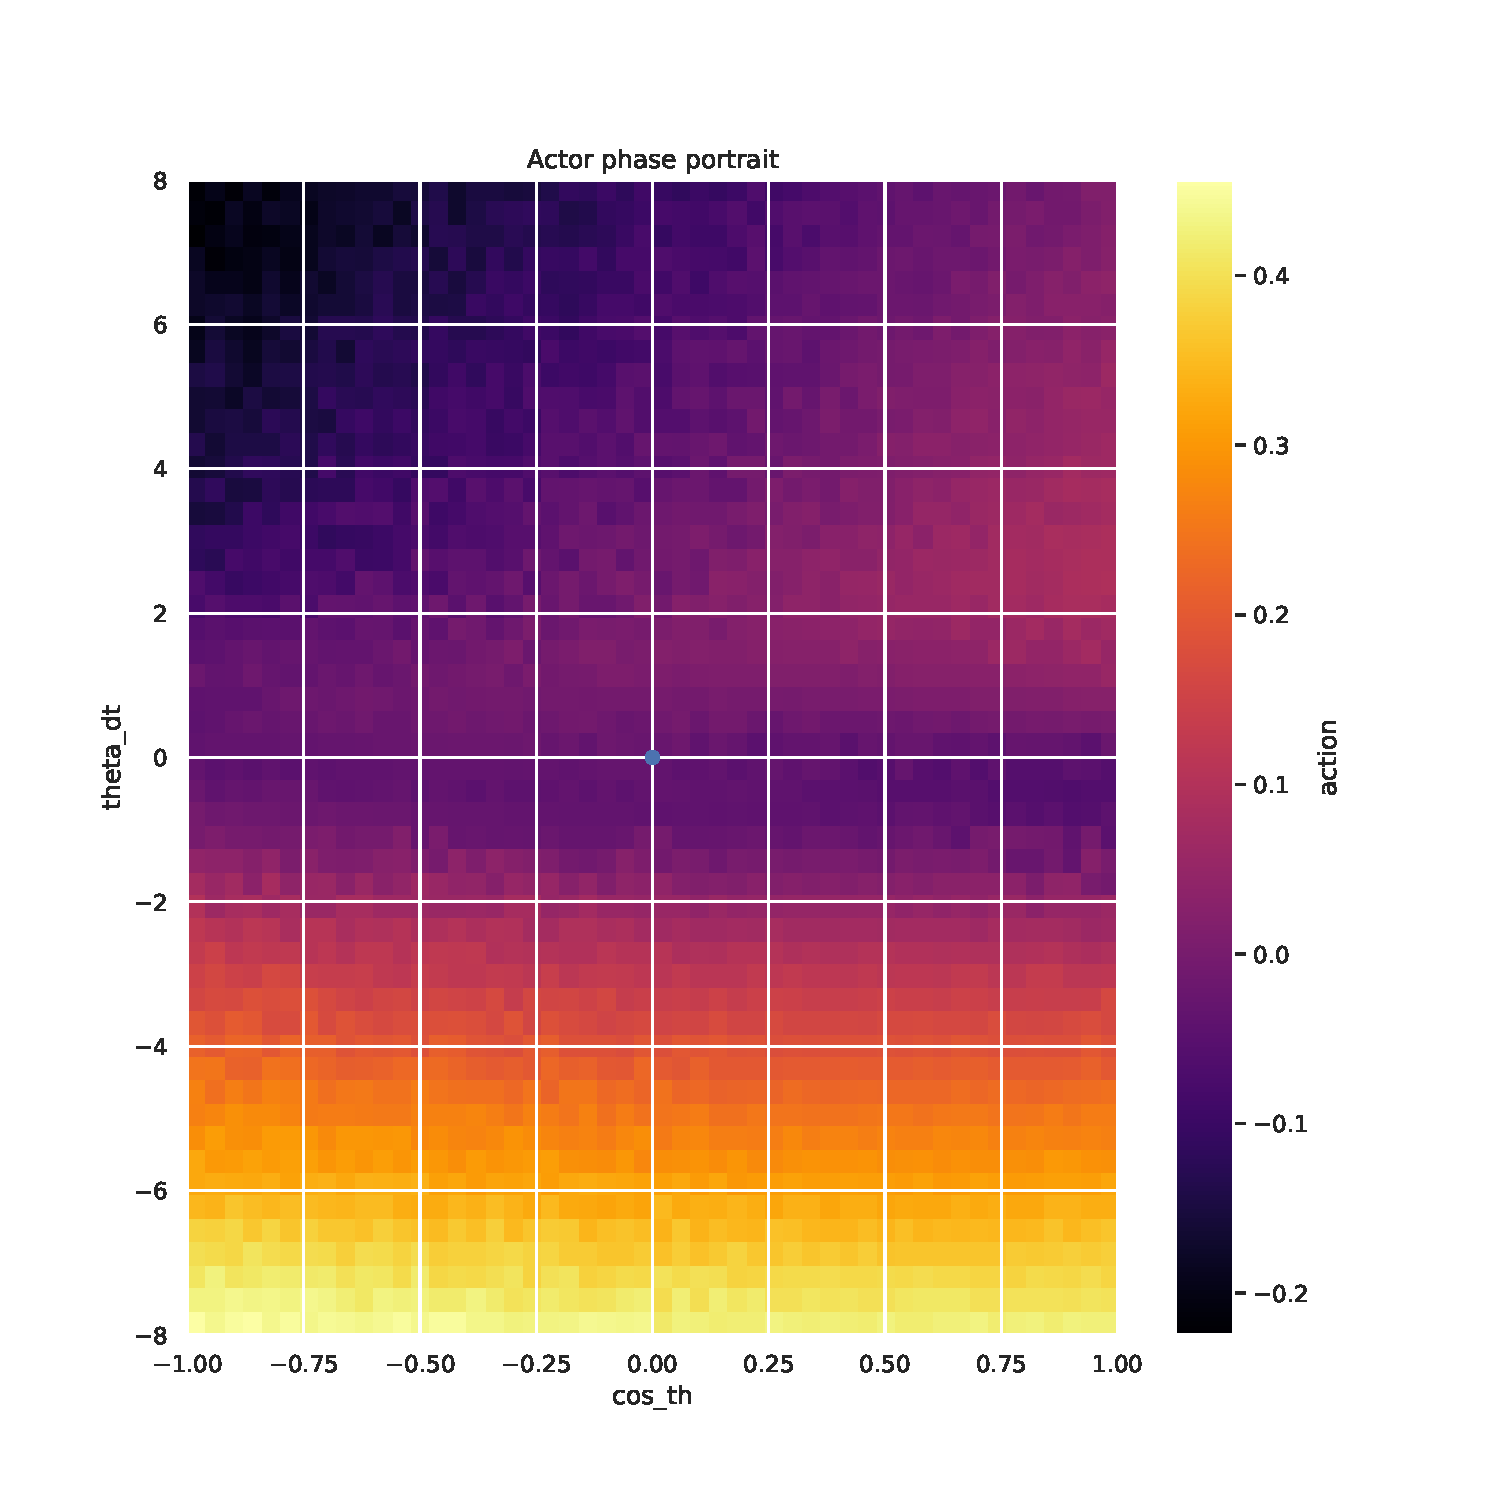
\includegraphics[width=\textwidth]{figures/prelimaire/0_actor_discount__ante_Pendulum-v0.pdf}
        \caption{Acteur naïf}
    \end{subfigure}
    \begin{subfigure}{0.3\textwidth}
        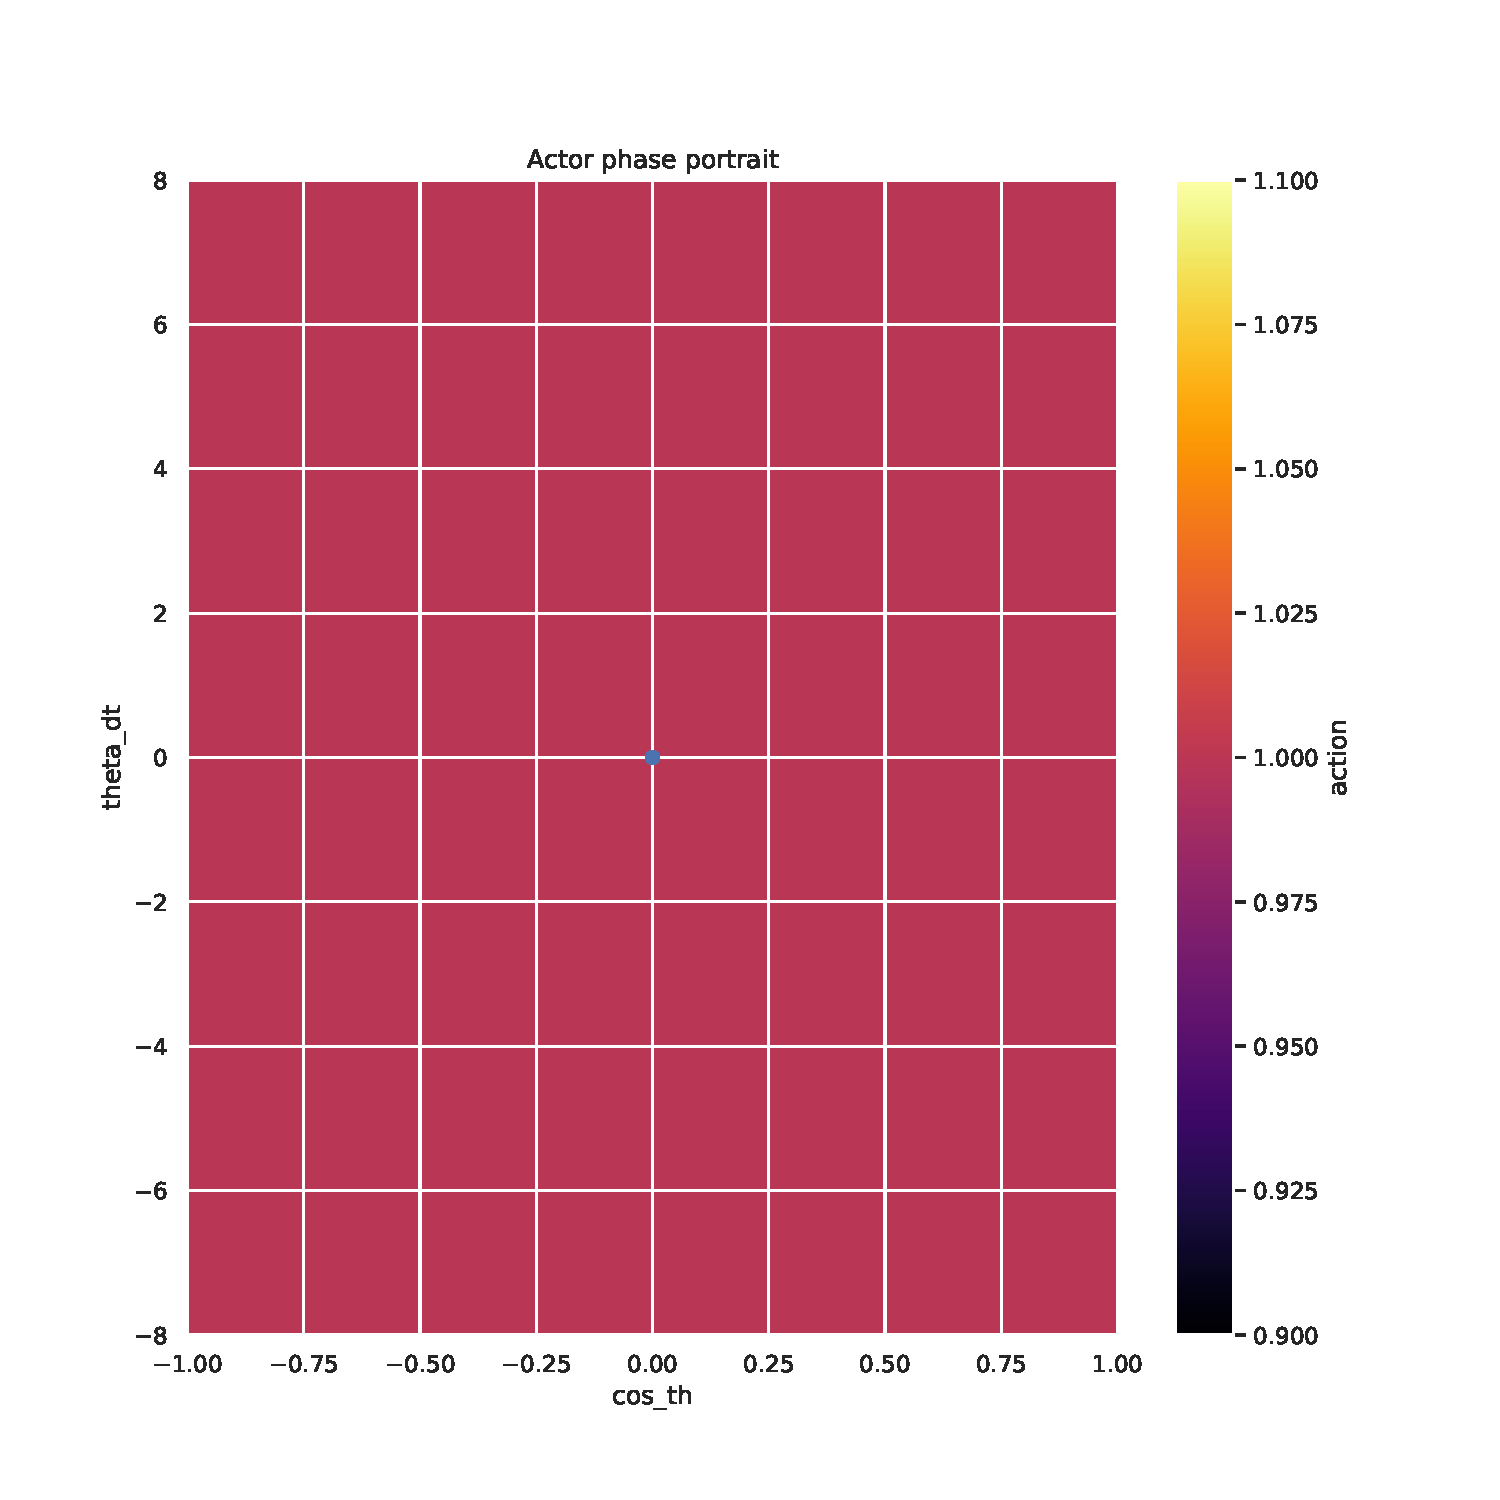
\includegraphics[width=\textwidth]{figures/prelimaire/0_actor_discount__post_Pendulum-v0.pdf}
        \caption{Acteur entraîné}
    \end{subfigure}
    \begin{subfigure}{0.3\textwidth}
        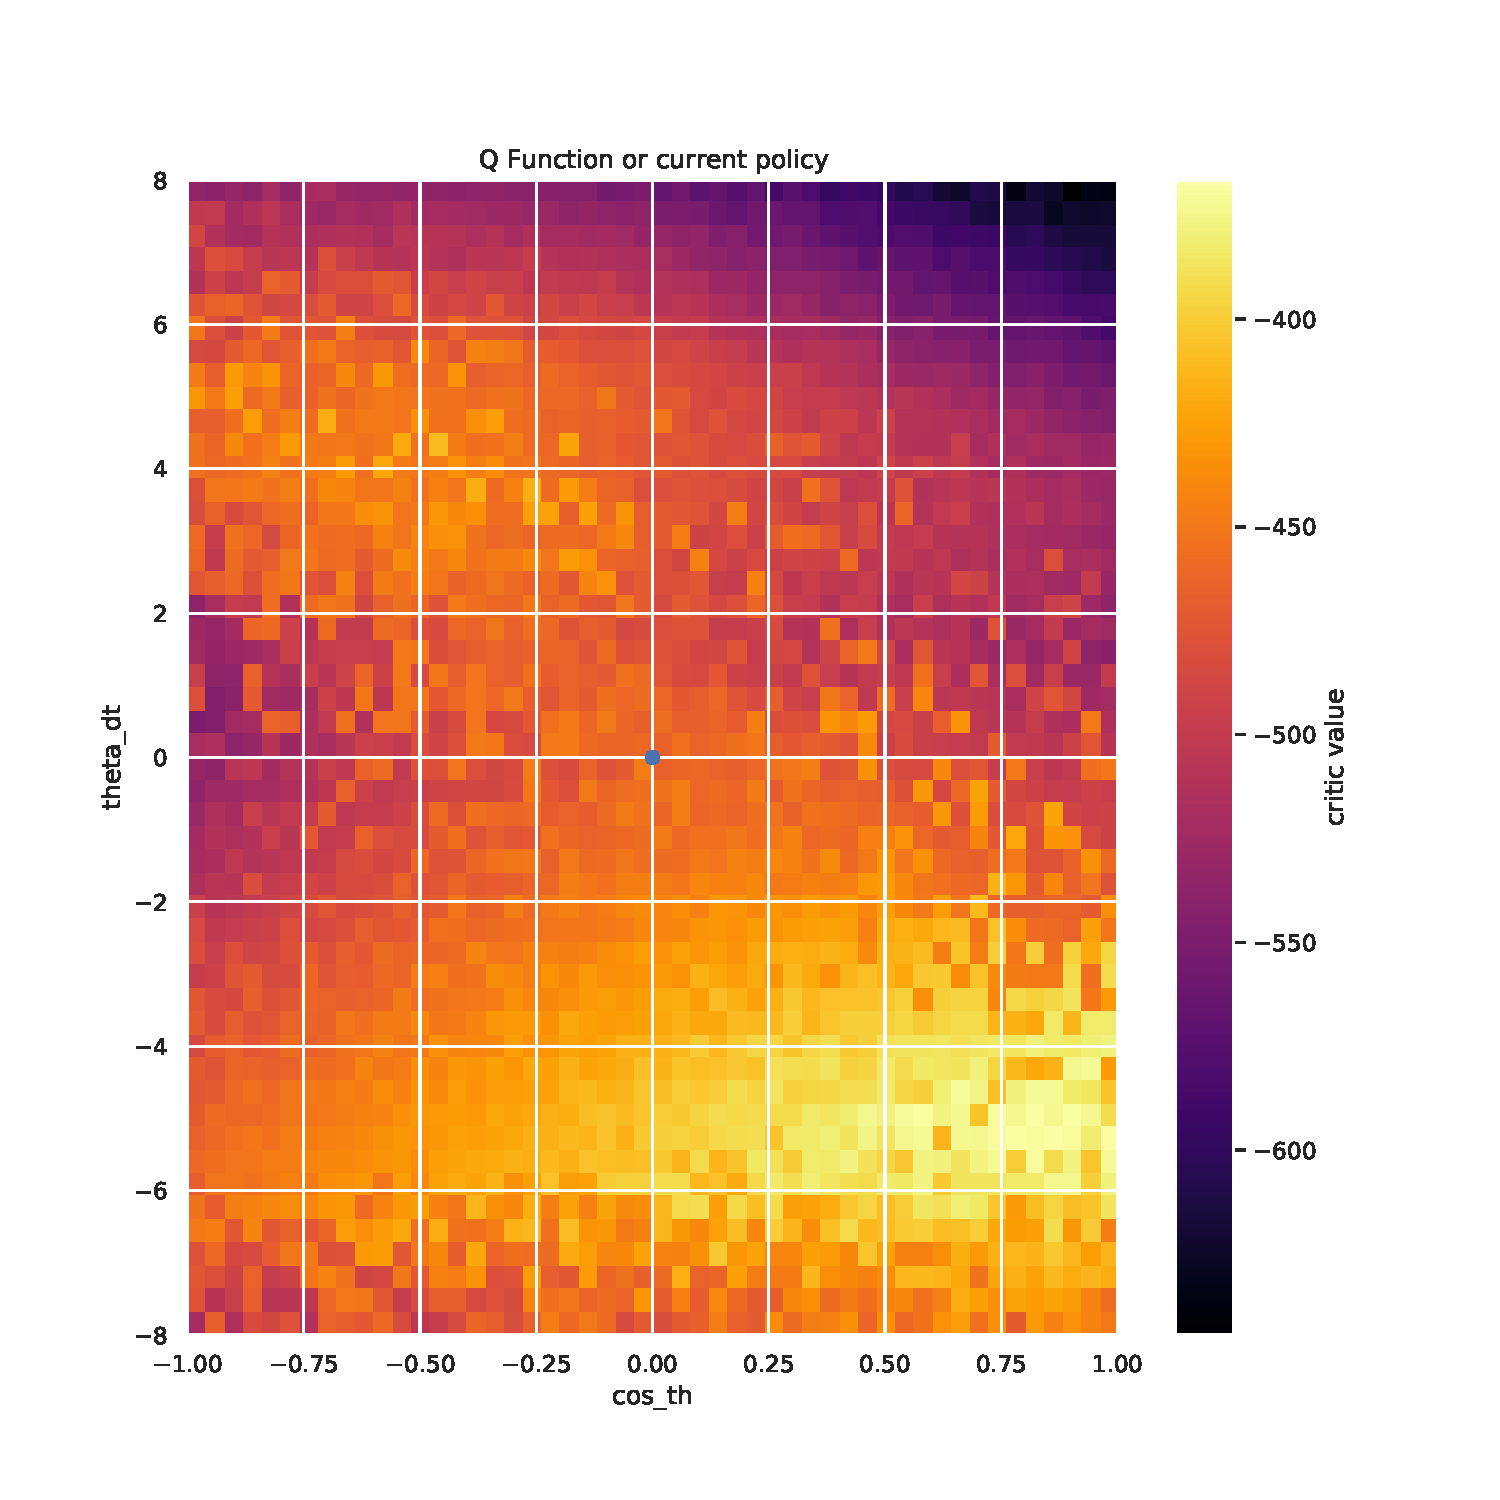
\includegraphics[width=\textwidth]{figures/prelimaire/0_critic_discount_post_Pendulum-v0.pdf}
        \caption{Critique entraînée}
    \end{subfigure}
    \caption{Valeurs de l'acteur et de la critique avec la méthode discount pour le calcul de la récompense}
    \label{fig:preli_discount}
\end{figure}

La figure~\ref{fig:preli_discount} nous montre un résultat aberrant où l'acteur converge vers une action uniforme à 1 sur l'ensemble des états qu'il peut atteindre. La \emph{heatmap} de la critique montre une préférence quand $\cos(\theta) = 1$ et c'est ce que nous voulons pour que le pendule reste à l'équilibre tout en haut. Mais nous observons aussi que la zone de préférence n'est pas pour $\dot{\theta} = 0$ alors que nous souhaitons que le pendule soit immobile à la position désirée.

\begin{figure}[H]
    \centering
    \begin{subfigure}{0.3\textwidth}
        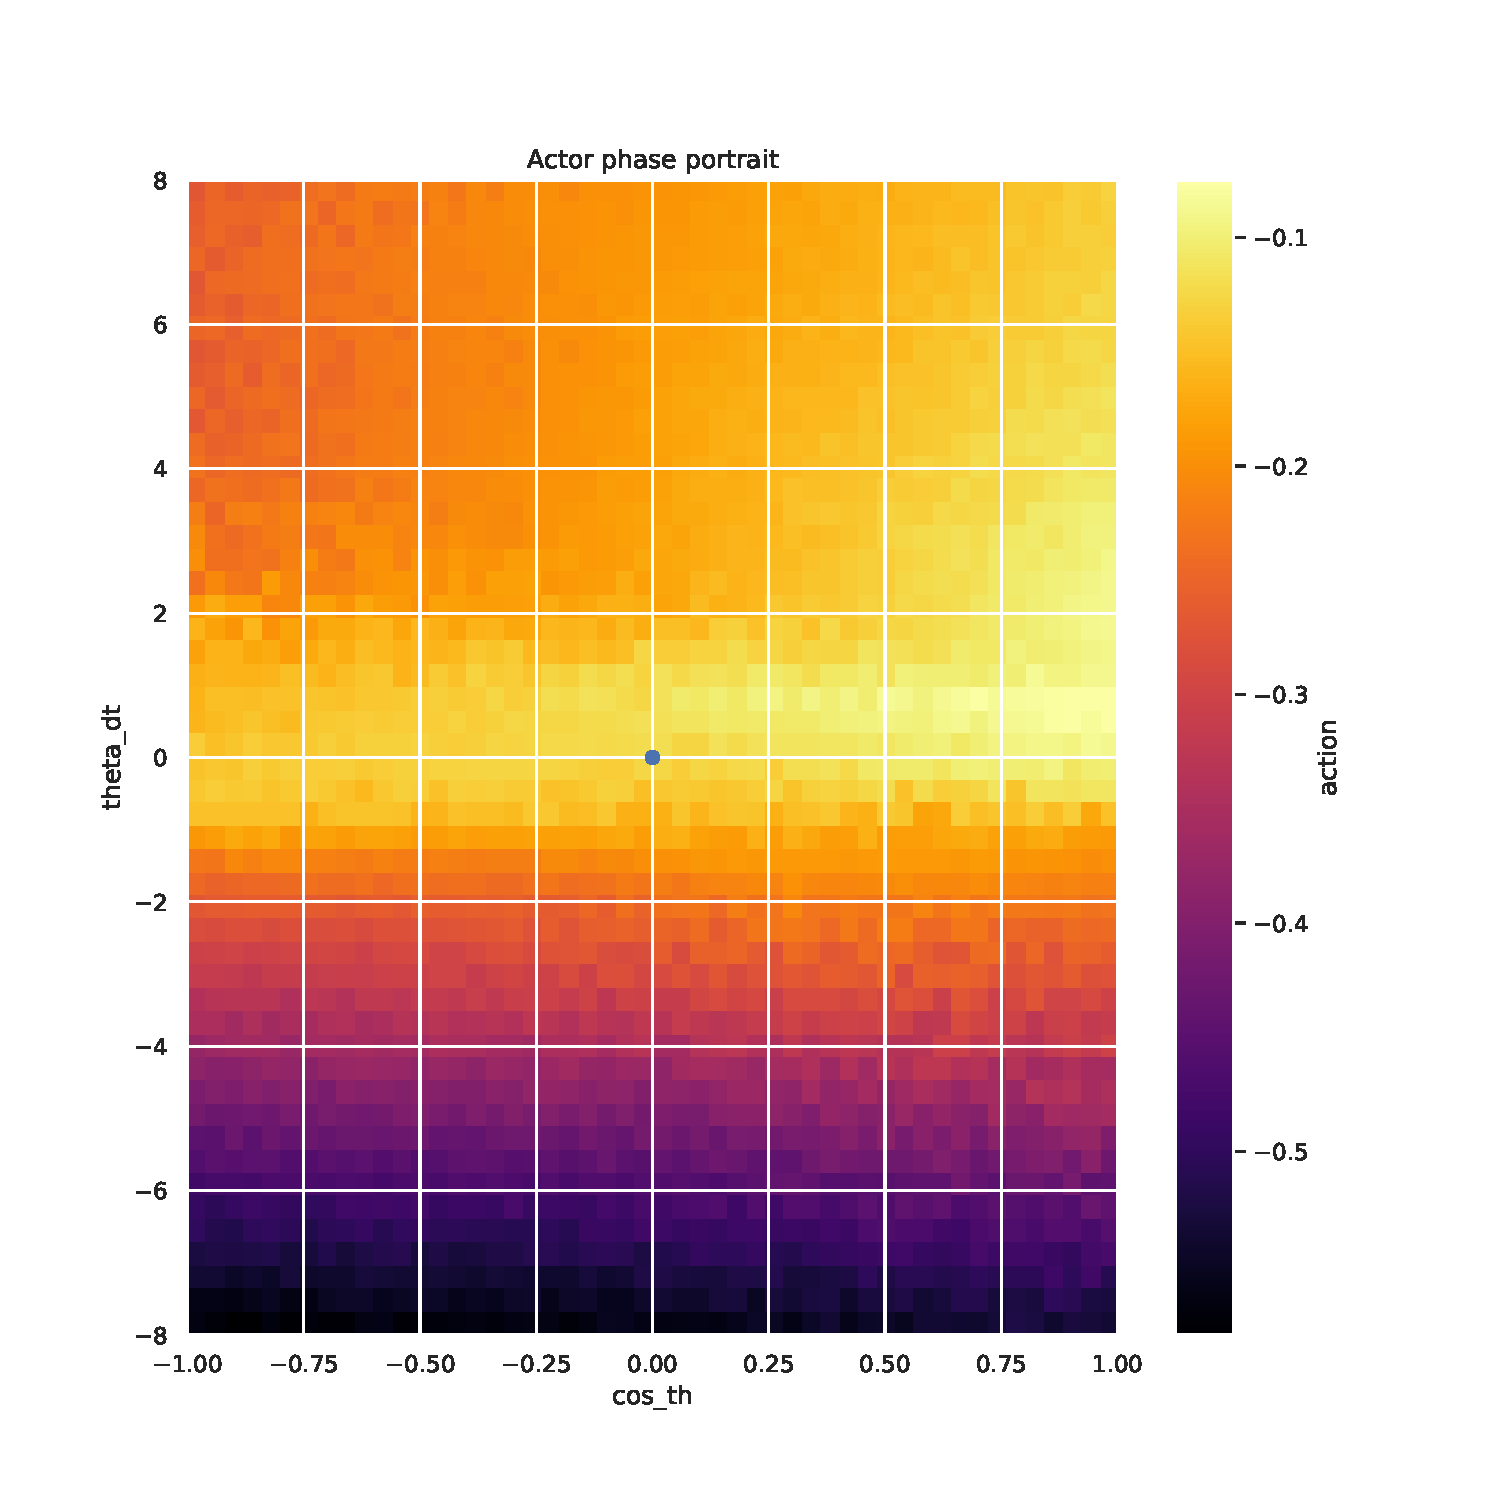
\includegraphics[width=\textwidth]{figures/prelimaire/0_actor_normalize__ante_Pendulum-v0.pdf}
        \caption{Acteur naïf}
    \end{subfigure}
    \begin{subfigure}{0.3\textwidth}
        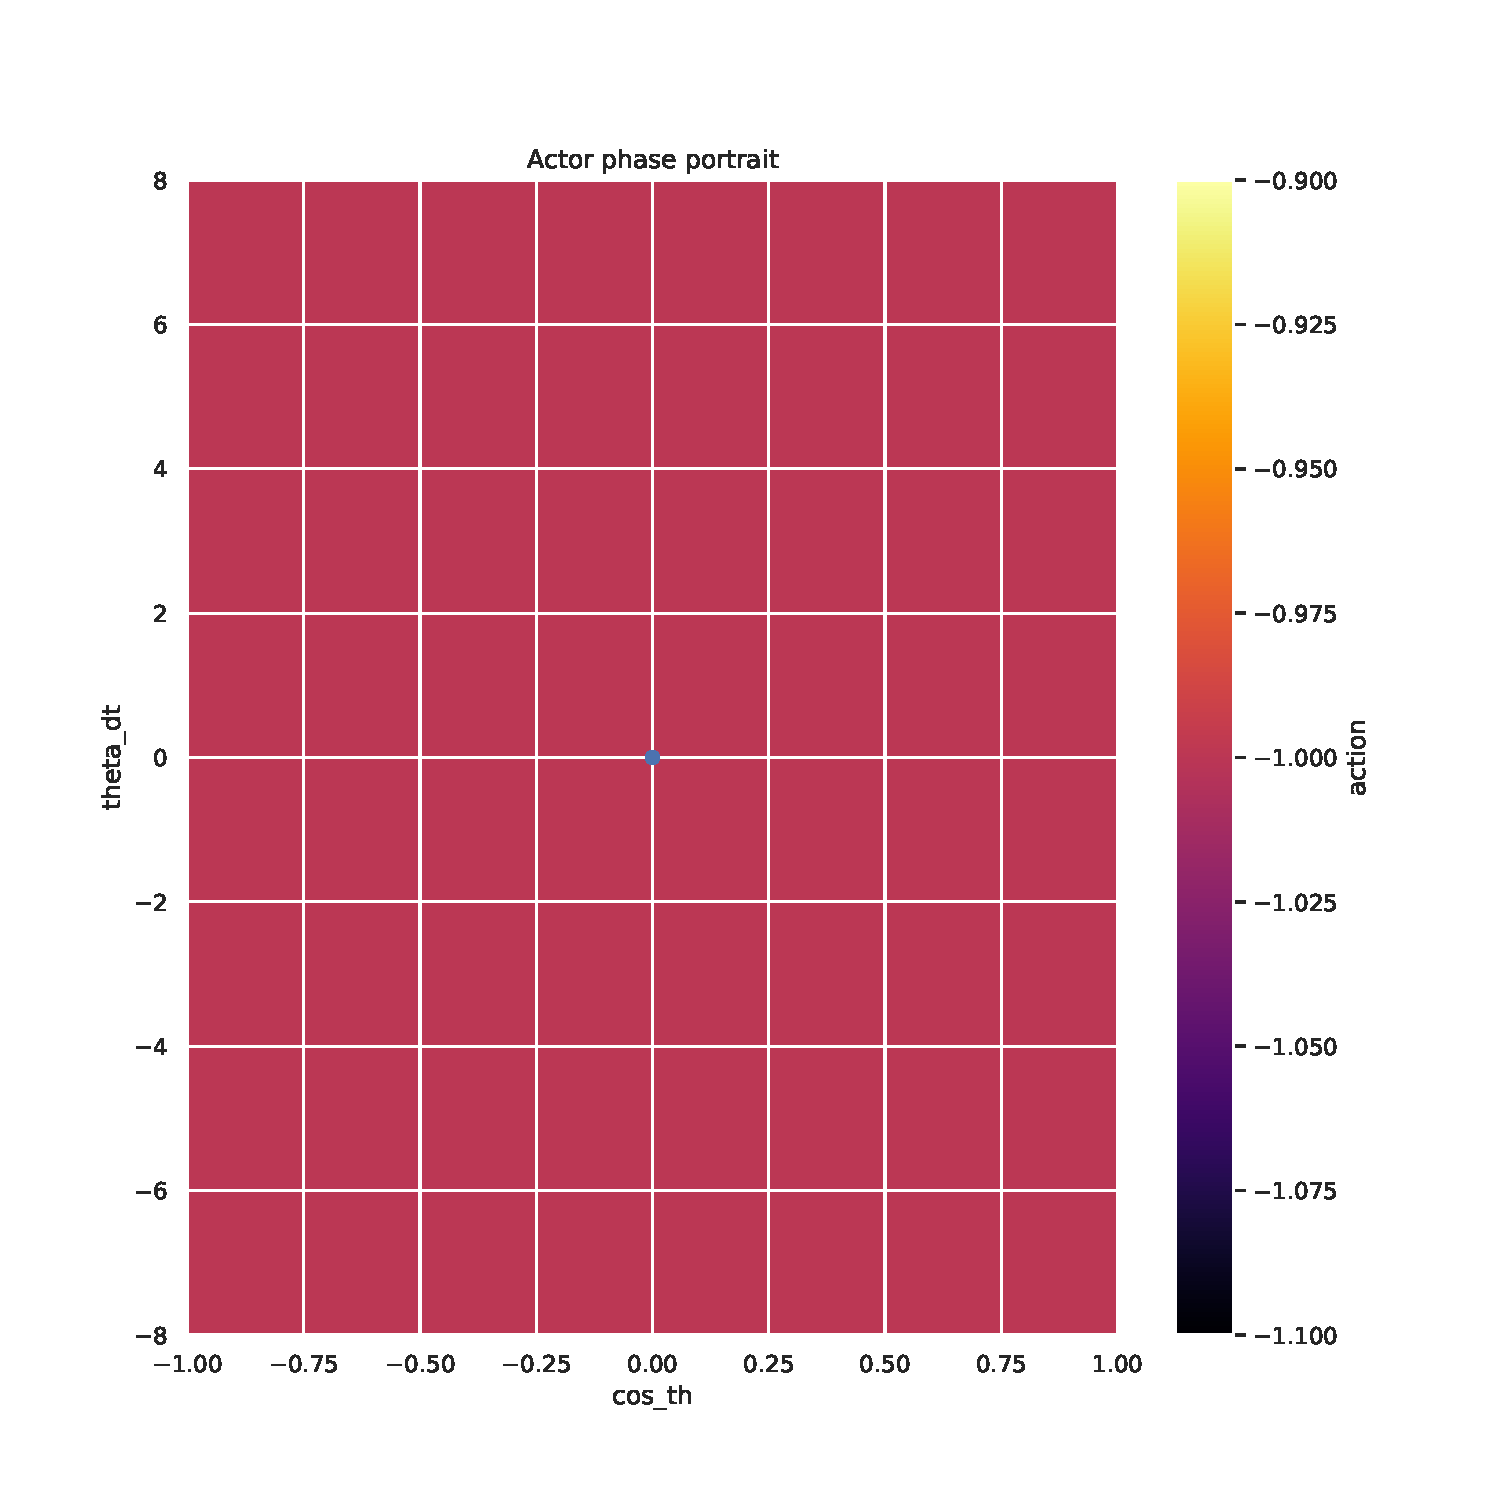
\includegraphics[width=\textwidth]{figures/prelimaire/0_actor_normalize__post_Pendulum-v0.pdf}
        \caption{Acteur entraîné}
    \end{subfigure}
    \begin{subfigure}{0.3\textwidth}
        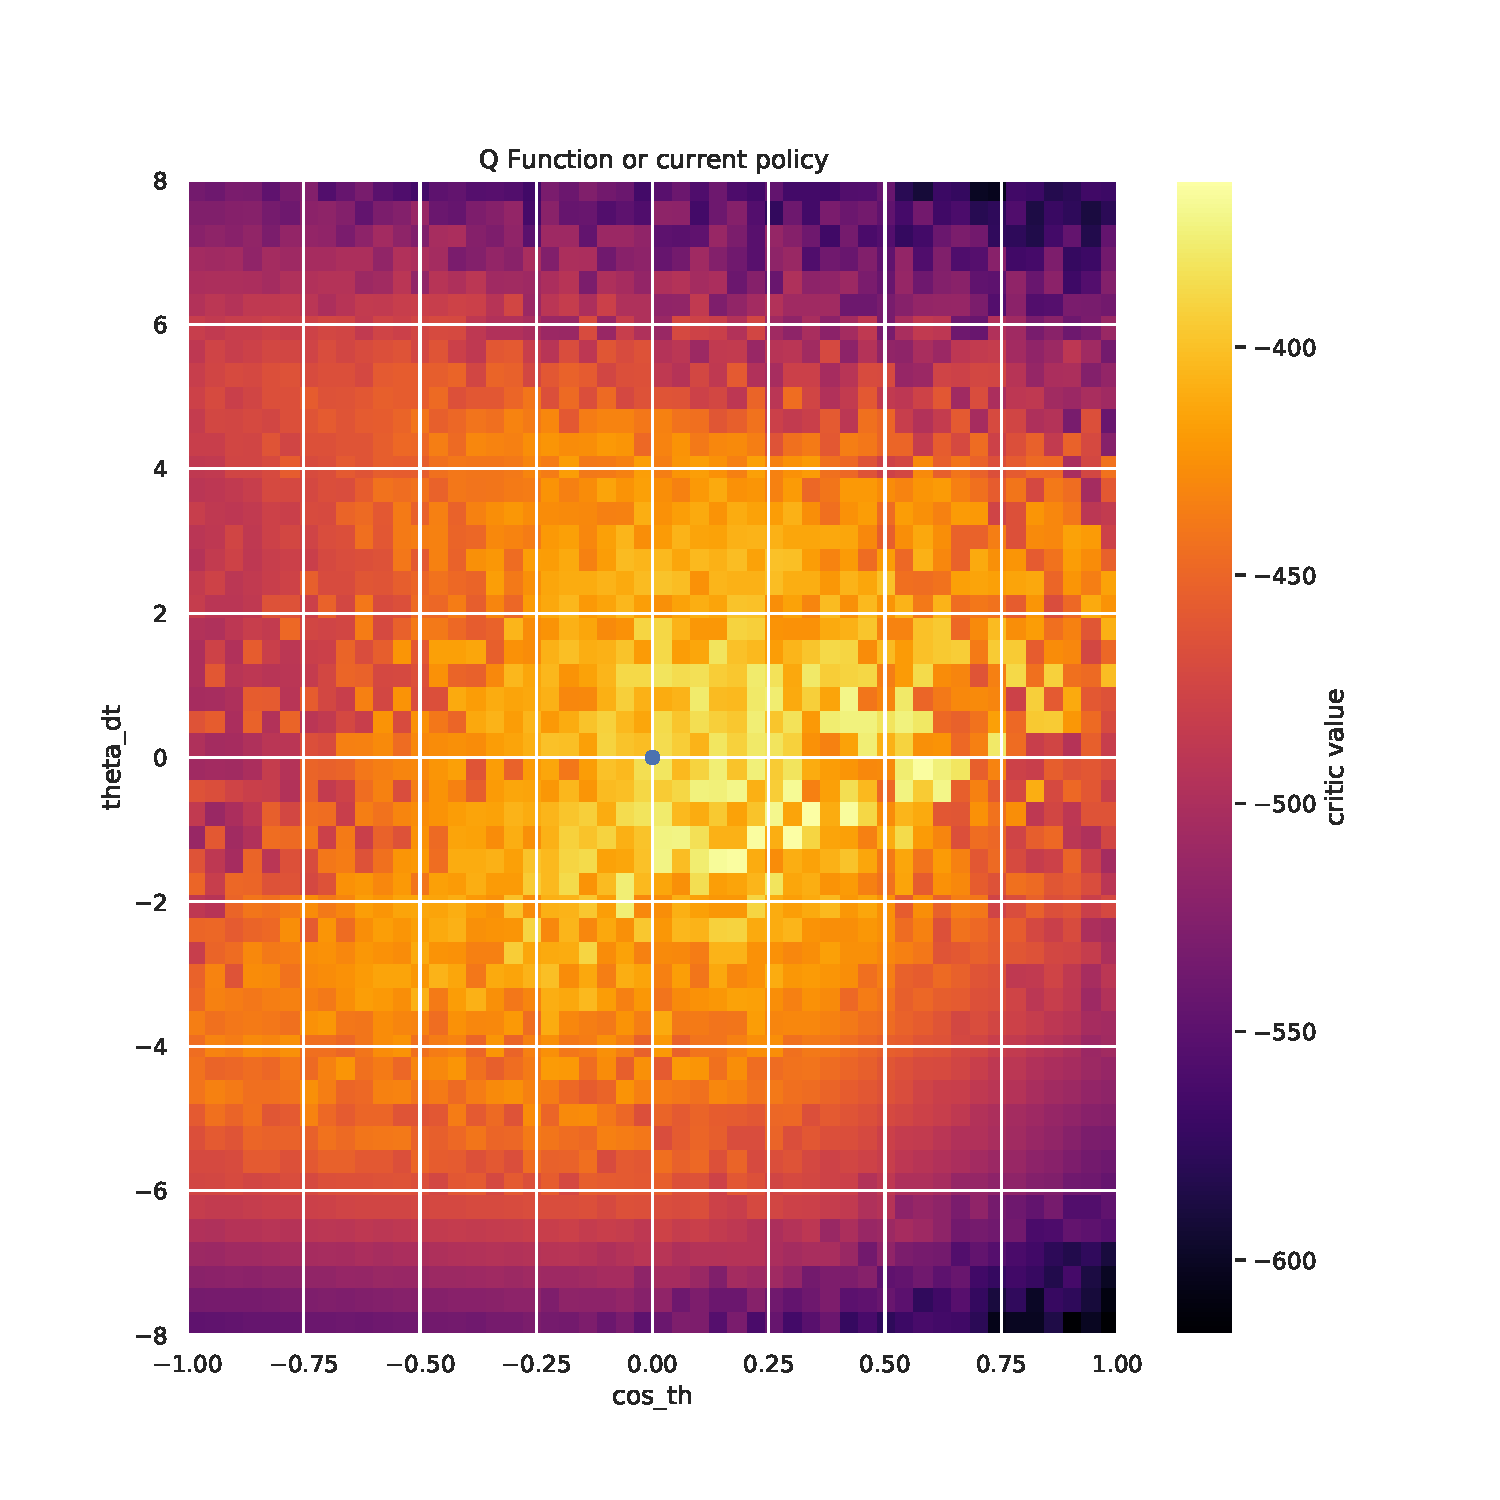
\includegraphics[width=\textwidth]{figures/prelimaire/0_critic_normalize_post_Pendulum-v0.pdf}
        \caption{Critique entraînée}
    \end{subfigure}
    \caption{Valeurs de l'acteur et de la critique avec la méthode normalise pour le calcul de la récompense}
    \label{fig:preli_normalise}
\end{figure}

La figure~\ref{fig:preli_normalise} montre le même problème pour l'acteur après entraînement où il converge vers 1 pour tous les états. Cependant, la préférence de $\dot{\theta}$ est bel et bien autour de 0 comme souhaité. Mais la valeur de préférence pour $\cos(\theta)$ n'est pas assez proche de 1 pour être caractérisée comme satisfaisante.

\begin{figure}[H]
    \centering
    \begin{subfigure}{0.3\textwidth}
        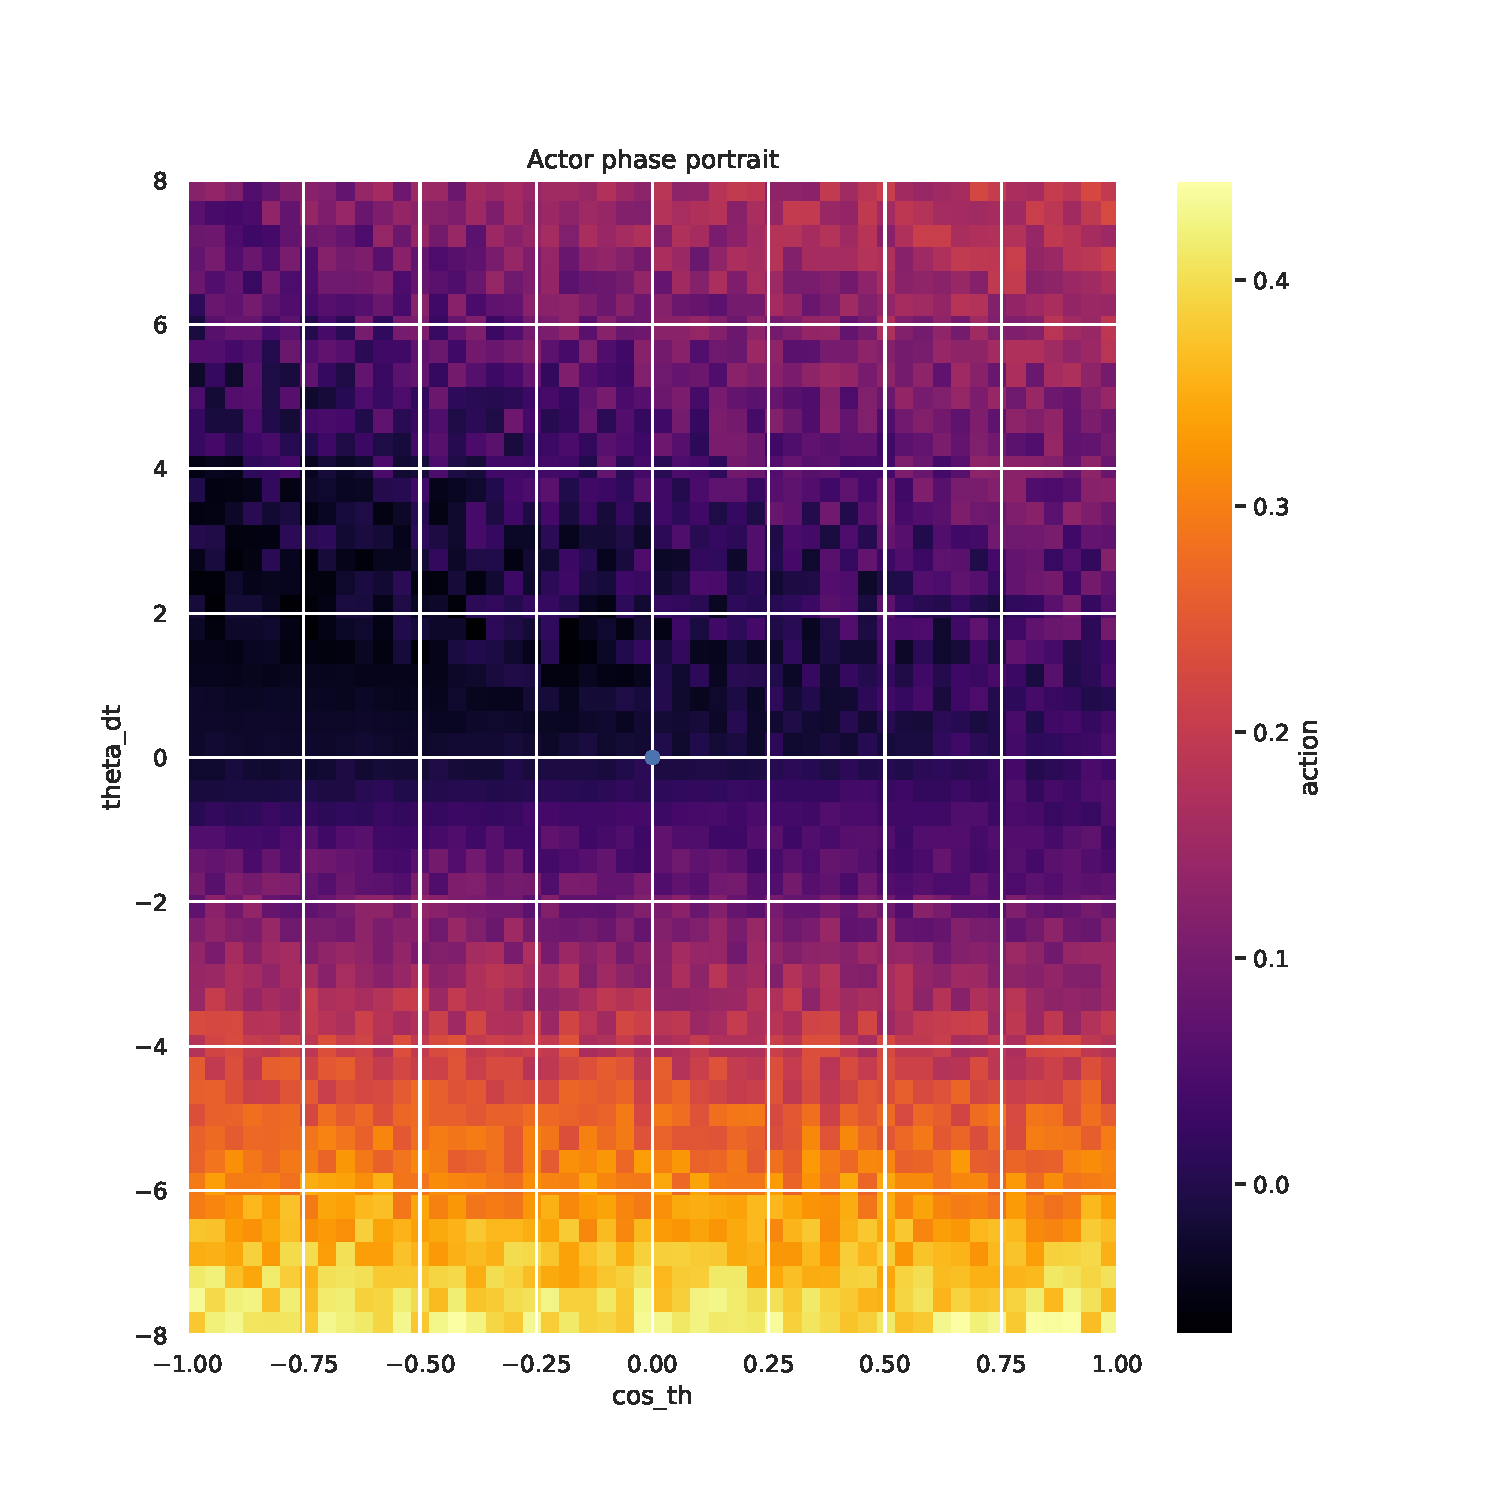
\includegraphics[width=\textwidth]{figures/prelimaire/0_actor_sum__ante_Pendulum-v0.pdf}
        \caption{Acteur naïf}
    \end{subfigure}
    \begin{subfigure}{0.3\textwidth}
        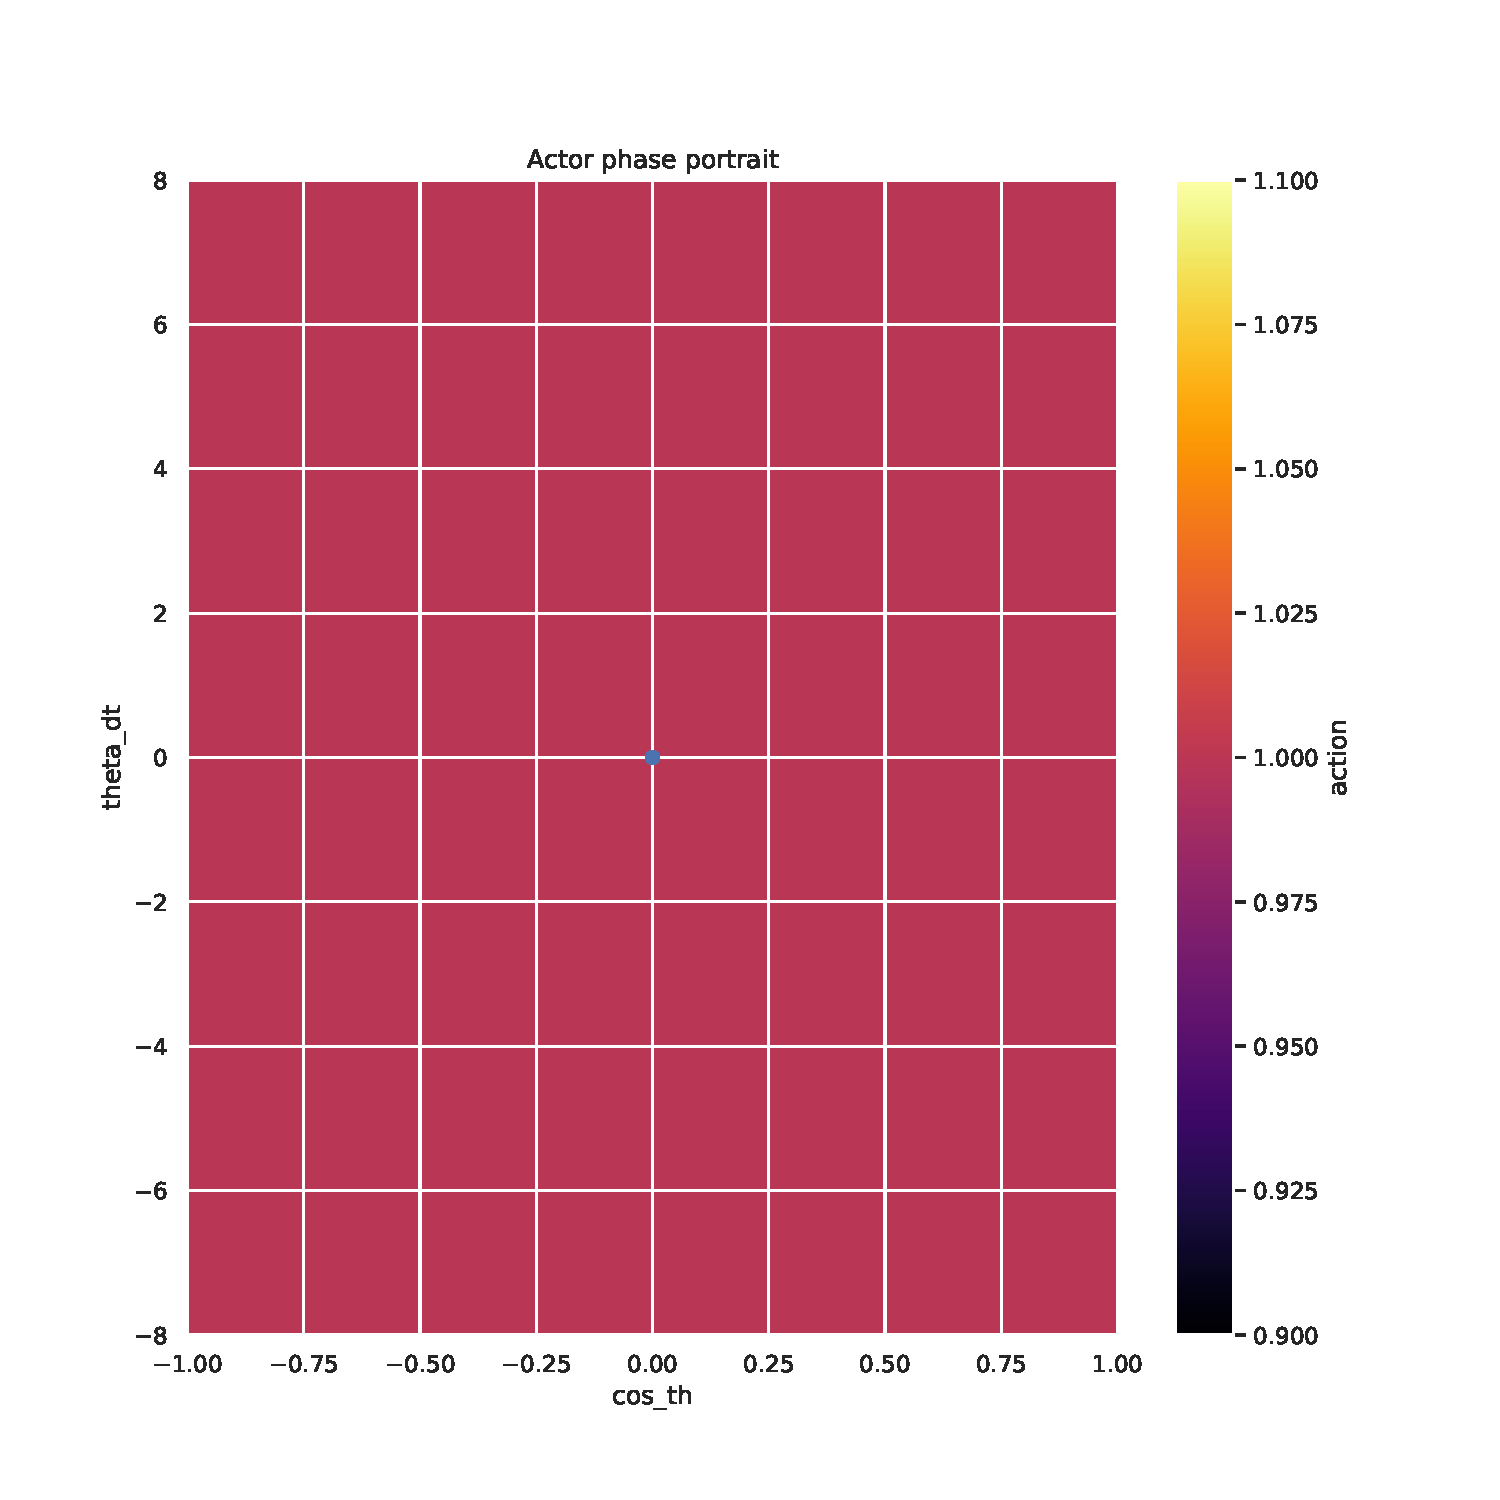
\includegraphics[width=\textwidth]{figures/prelimaire/0_actor_sum__post_Pendulum-v0.pdf}
        \caption{Acteur entraîné}
    \end{subfigure}
    \begin{subfigure}{0.3\textwidth}
        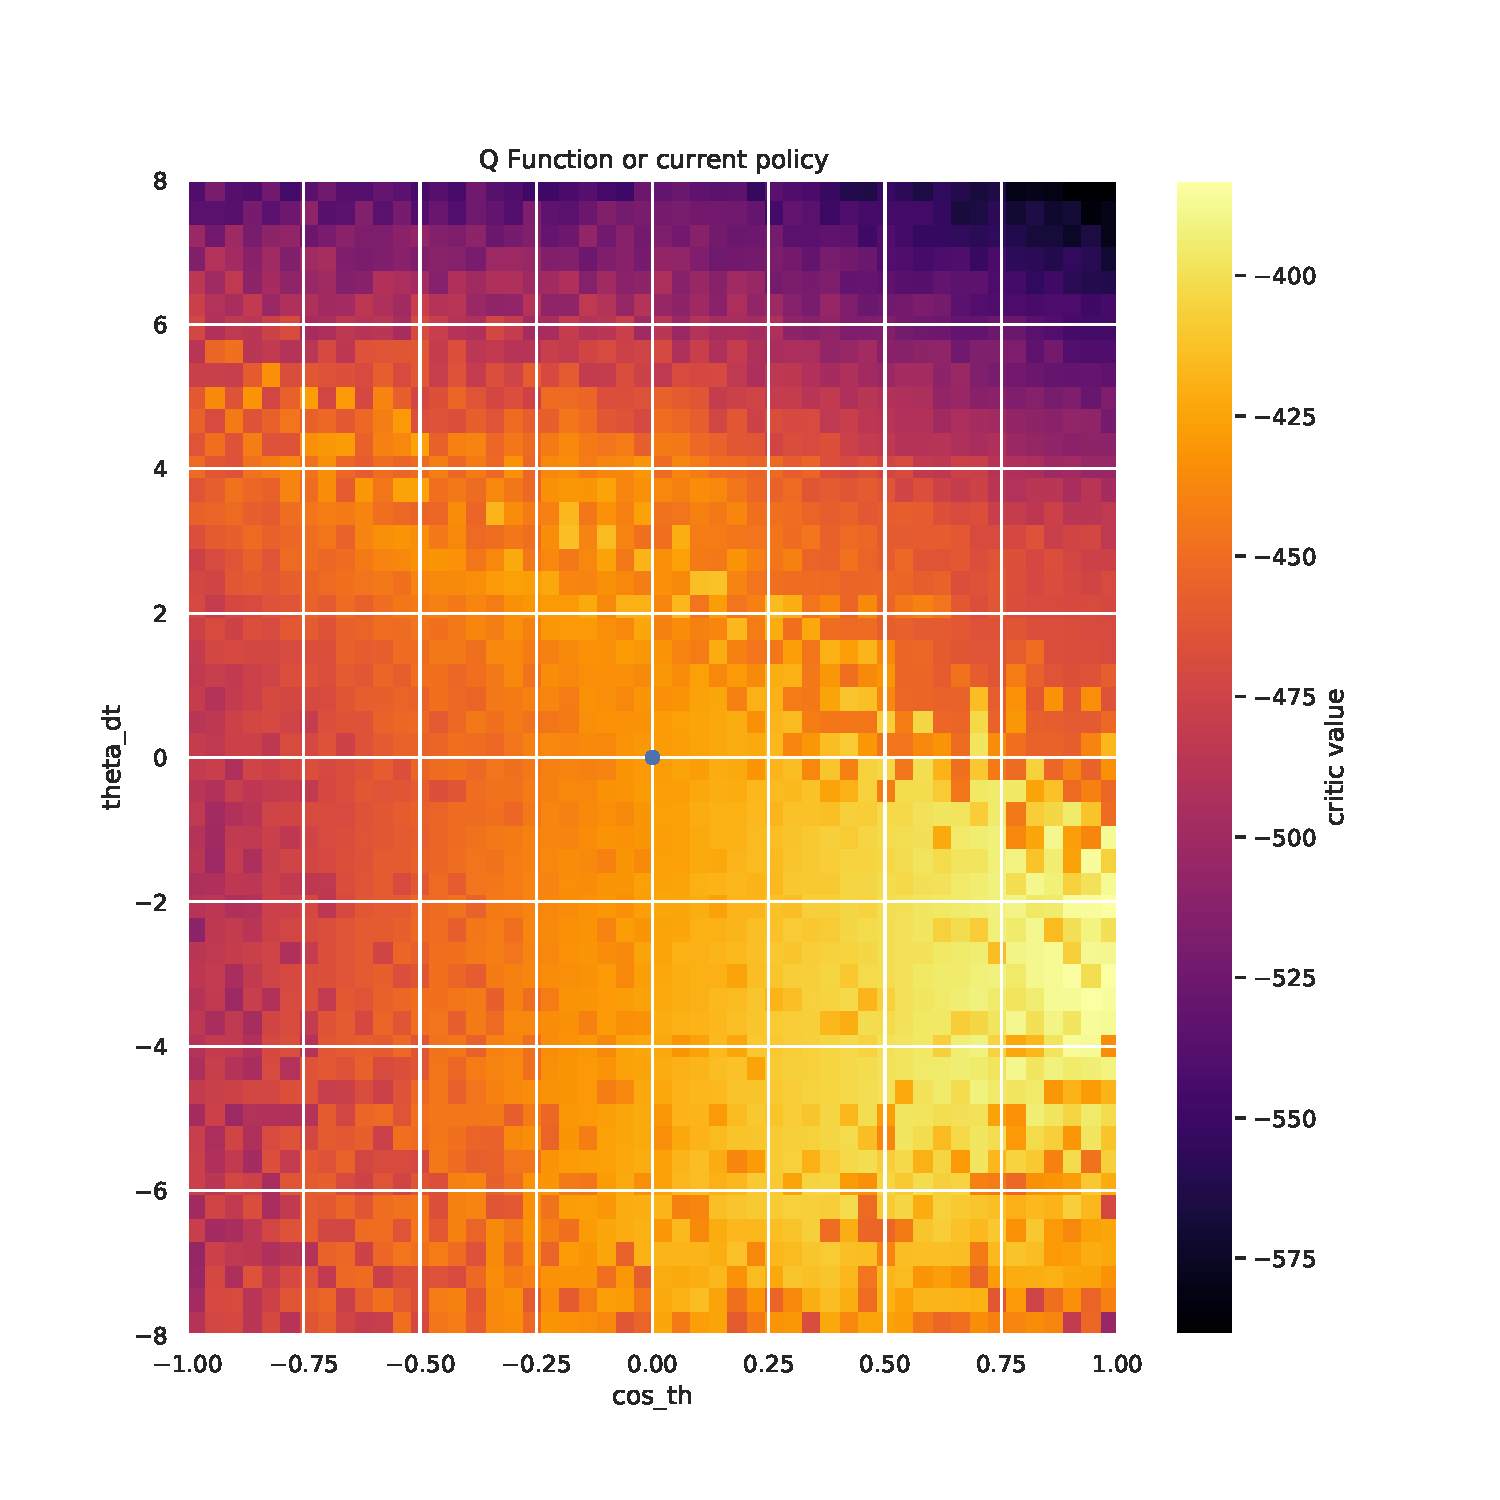
\includegraphics[width=\textwidth]{figures/prelimaire/0_critic_sum_post_Pendulum-v0.pdf}
        \caption{Critique entraînée}
    \end{subfigure}
    \caption{Valeurs de l'acteur et de la critique avec la méthode de sommation pour le calcul de la récompense}
    \label{fig:preli_sum}
\end{figure}

La figure~\ref{fig:preli_sum} présente également le résultat absurde sur l'acteur entraîné uniforme et unitaire sur l'ensemble des états. Nous observons par contre une zone de préférence pour $\cos(\theta) = 1$, c'est à dire la position souhaitée du pendule. Mais ici encore, pour $\dot{\theta}$, la zone de préférence n'est pas encore assez proche de 0 pour être satisfaisante.

Pour les trois méthodes de calcul de la récompense sur une trajectoire, la critique ne présente pas un maximum pour les états optimaux. Nous remarquons que les zones chaudes sont très vastes. Nous en déduisons que la critique est de mauvaise qualité par manque d'exploration.

La récompense maximale est estimée pour $\dot{\theta} \not= 0$. Donc l'agent n'a vu cette récompense que lorsque qu'il poussait à pleine vitesse. Ainsi le gradient de la critique a poussé la politique à toujours utiliser le couple maximum. D'où le fait que les acteurs renvoient toujours $1$ (soit le couple maximum dans le sens direct).

\section{Itérations de simulation}
\subsection{Itération n°1}

\subsubsection{Configuration et modifications}

Nous décidons de ne plus utiliser de \emph{squashed gaussian} dans l'évaluation de l'acteur. Cela nous permet de voir plus finement le comportement de la distribution normal que cache la fonction tangente hyperbolique. A la place, nous choisissons de calculer l'action à partir d'une distribution normale dont l'écart-type est imposé à $1,5$ pour qu'il y ait de l'exploration en tout temps.

Nous décidons de ne plus calculer le gradient par sommation des récompenses pour réduire le temps de calcul.

\subsubsection{Analyse}

\begin{figure}[H]
    \centering
    \begin{subfigure}{0.3\textwidth}
        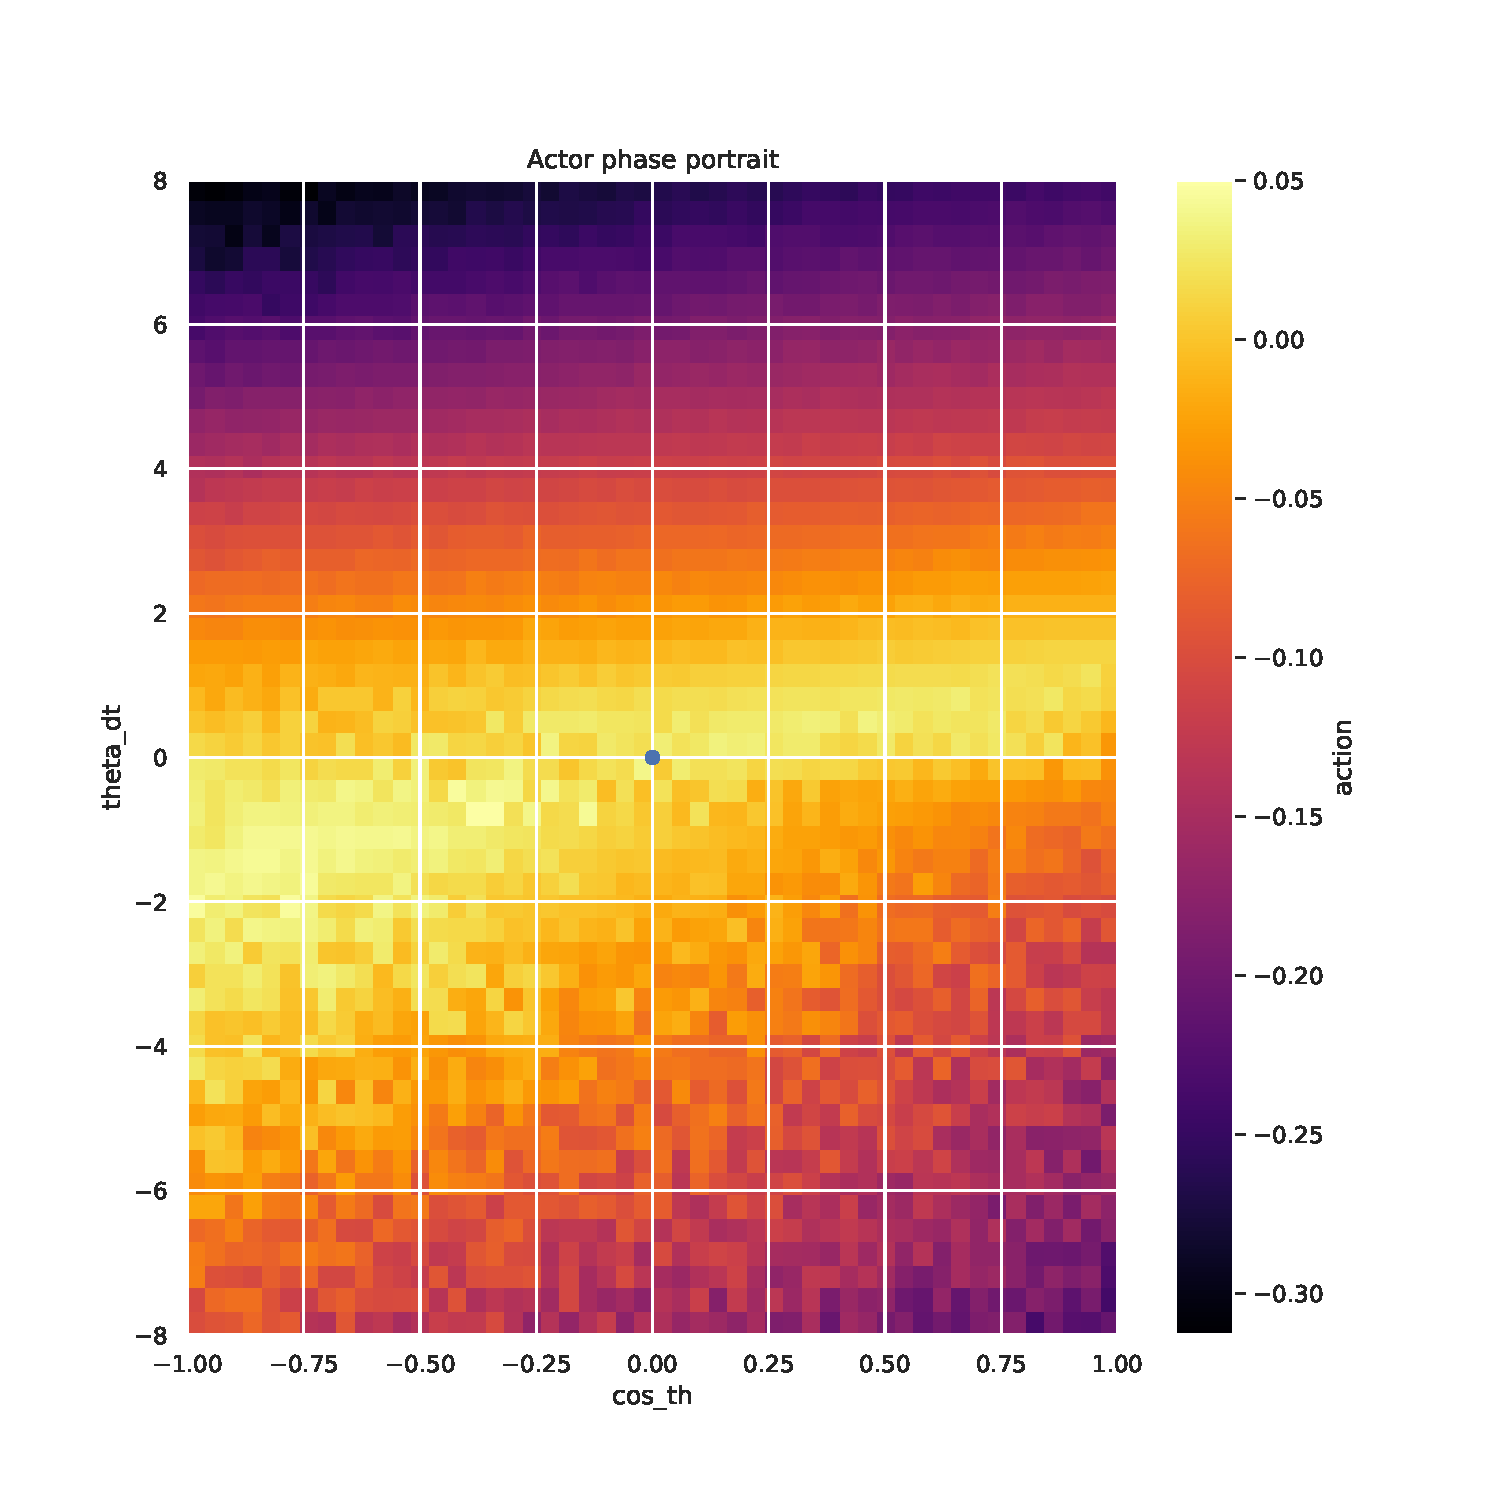
\includegraphics[width=\textwidth]{figures/iteration1/0_actor_discount__ante_Pendulum-v0.pdf}
        \caption{Acteur naïf}
    \end{subfigure}
    \begin{subfigure}{0.3\textwidth}
        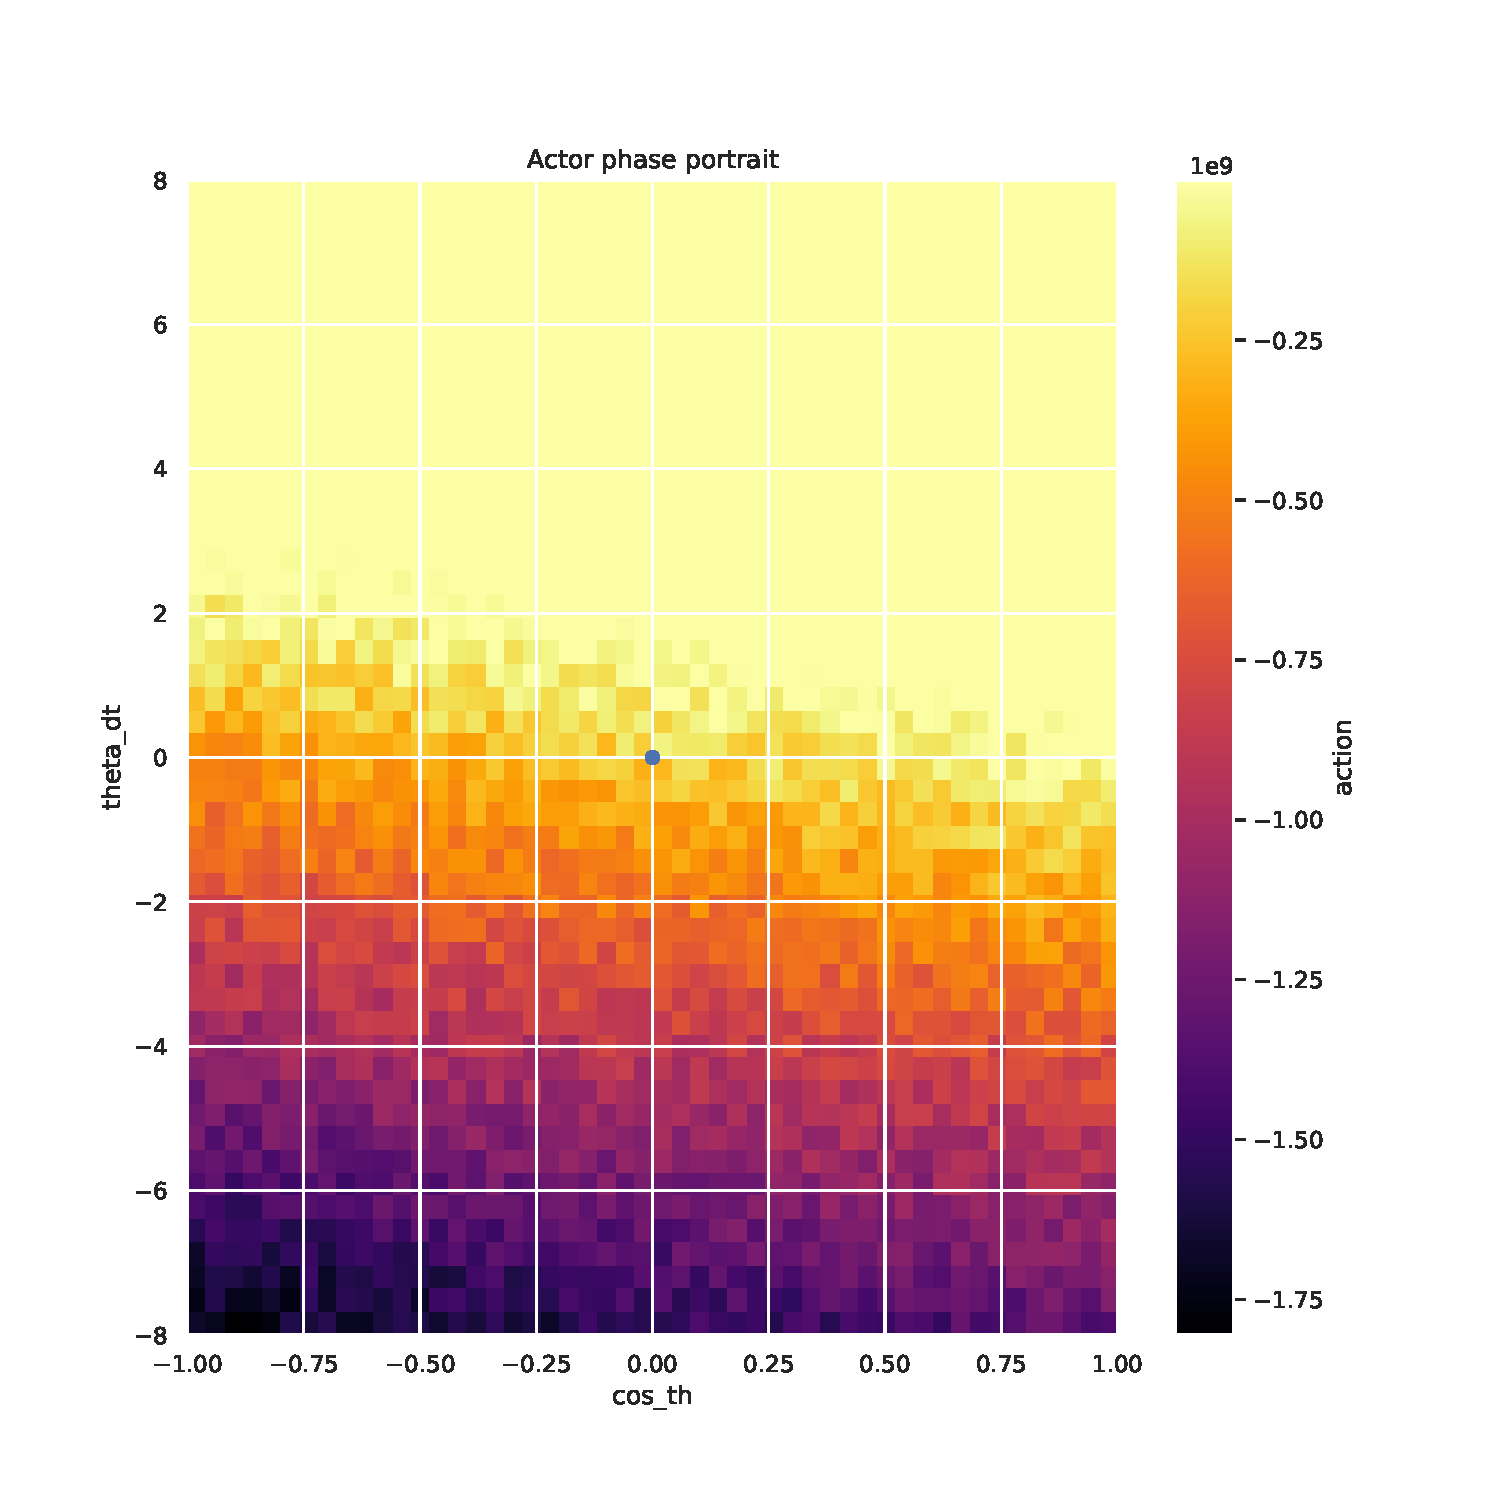
\includegraphics[width=\textwidth]{figures/iteration1/0_actor_discount__post_Pendulum-v0.pdf}
        \caption{Acteur entraîné}
    \end{subfigure}
    \begin{subfigure}{0.3\textwidth}
        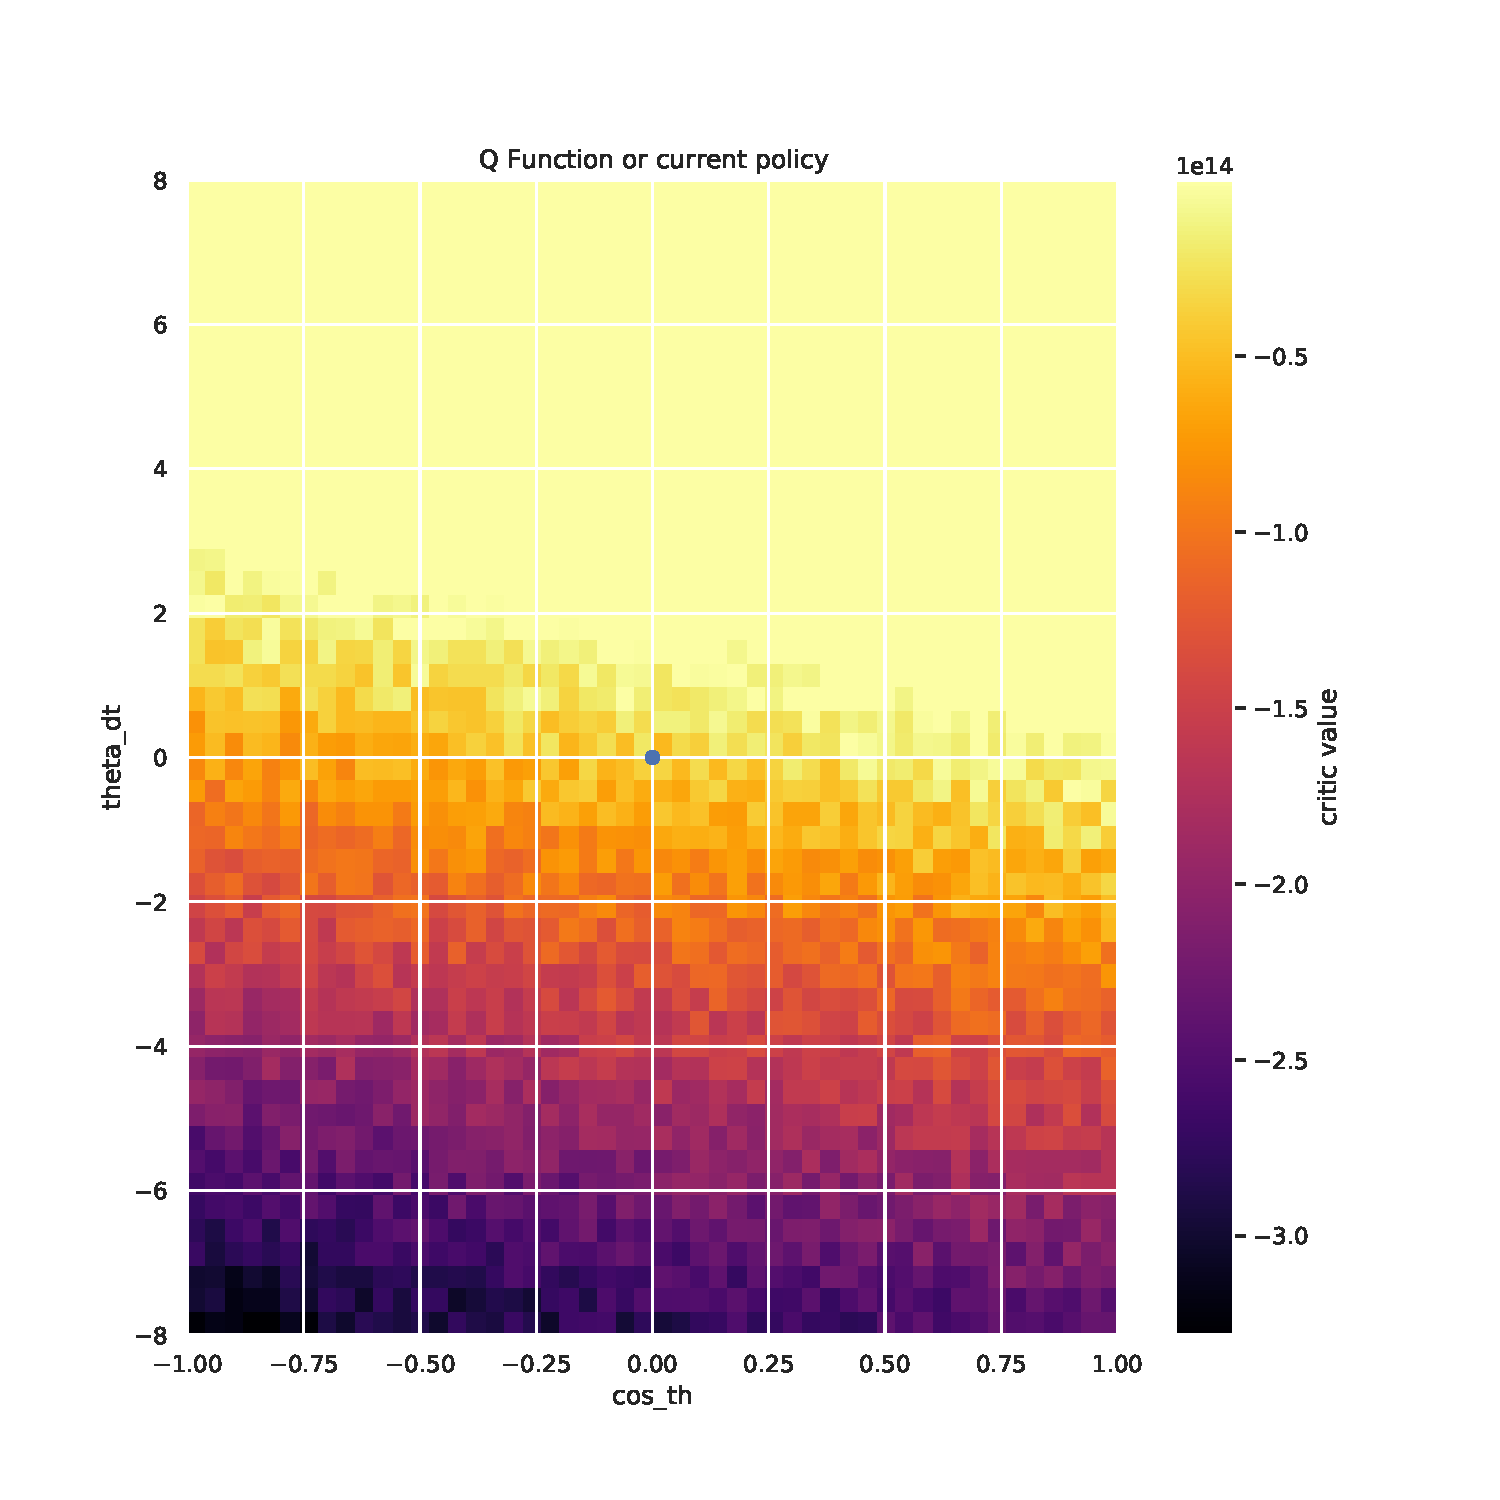
\includegraphics[width=\textwidth]{figures/iteration1/0_critic_discount_post_Pendulum-v0.pdf}
        \caption{Critique entraînée}
    \end{subfigure}
    \caption{Valeurs de l'acteur et de la critique avec la méthode discount pour le calcul de la récompense}
    \label{fig:attempt1_disount}
\end{figure}

Avec l'évaluation de l'acteur \emph{normal} dans la figure~\ref{fig:attempt1_disount}, la critique et l'acteur obtenus après entraînement sont quasiment identiques. Mais les \emph{heatmaps} de ces derniers ne sont pas du tout satisfaisantes. En effet, la zone de préférence est située dans l'intervalle positif des vitesses angulaires. Or nous souhaitons que l'IA favorise une position d'équilibre en haut du pendule.

\begin{figure}[H]
    \centering
    \begin{subfigure}{0.3\textwidth}
        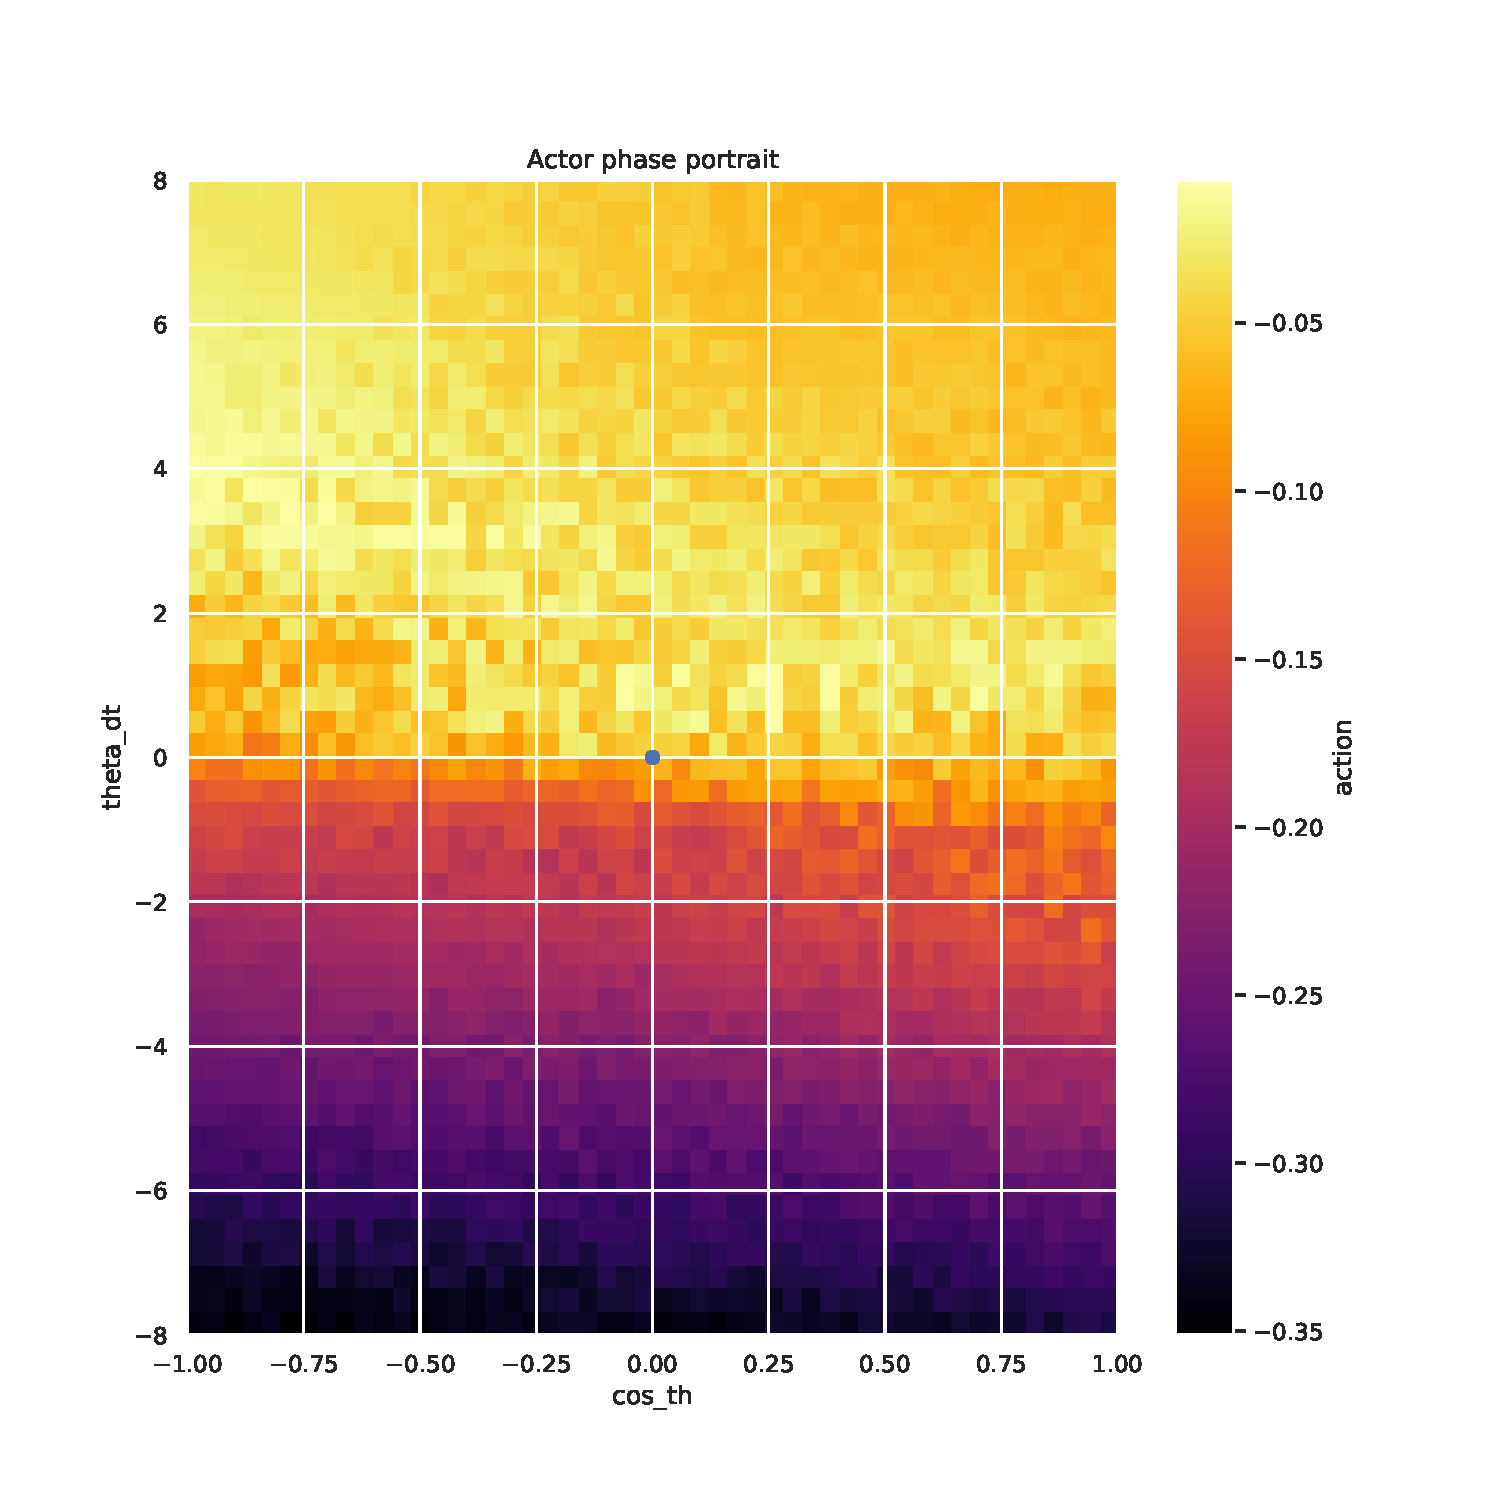
\includegraphics[width=\textwidth]{figures/iteration1/0_actor_normalize__ante_Pendulum-v0.pdf}
        \caption{Acteur naïf}
    \end{subfigure}
    \begin{subfigure}{0.3\textwidth}
        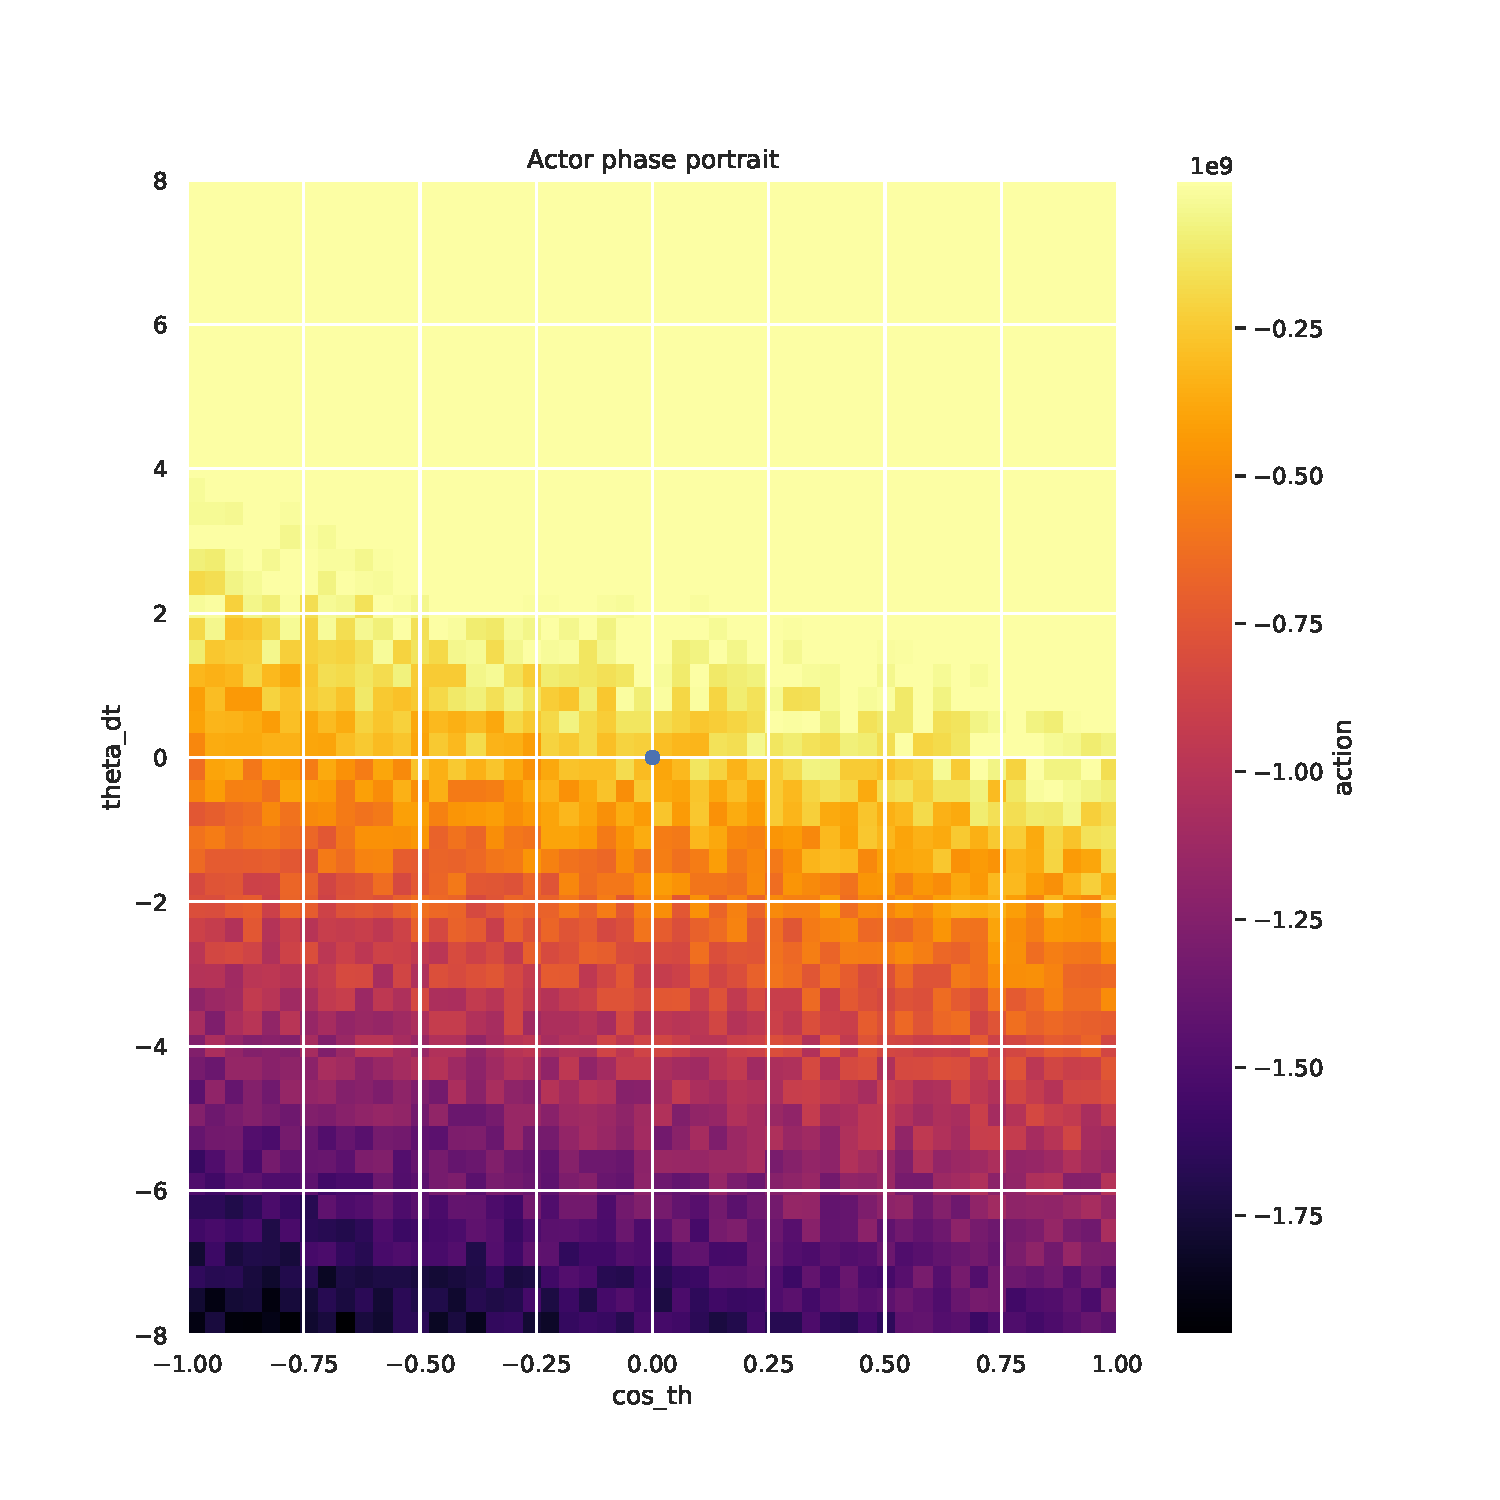
\includegraphics[width=\textwidth]{figures/iteration1/0_actor_normalize__post_Pendulum-v0.pdf}
        \caption{Acteur entraîné}
    \end{subfigure}
    \begin{subfigure}{0.3\textwidth}
        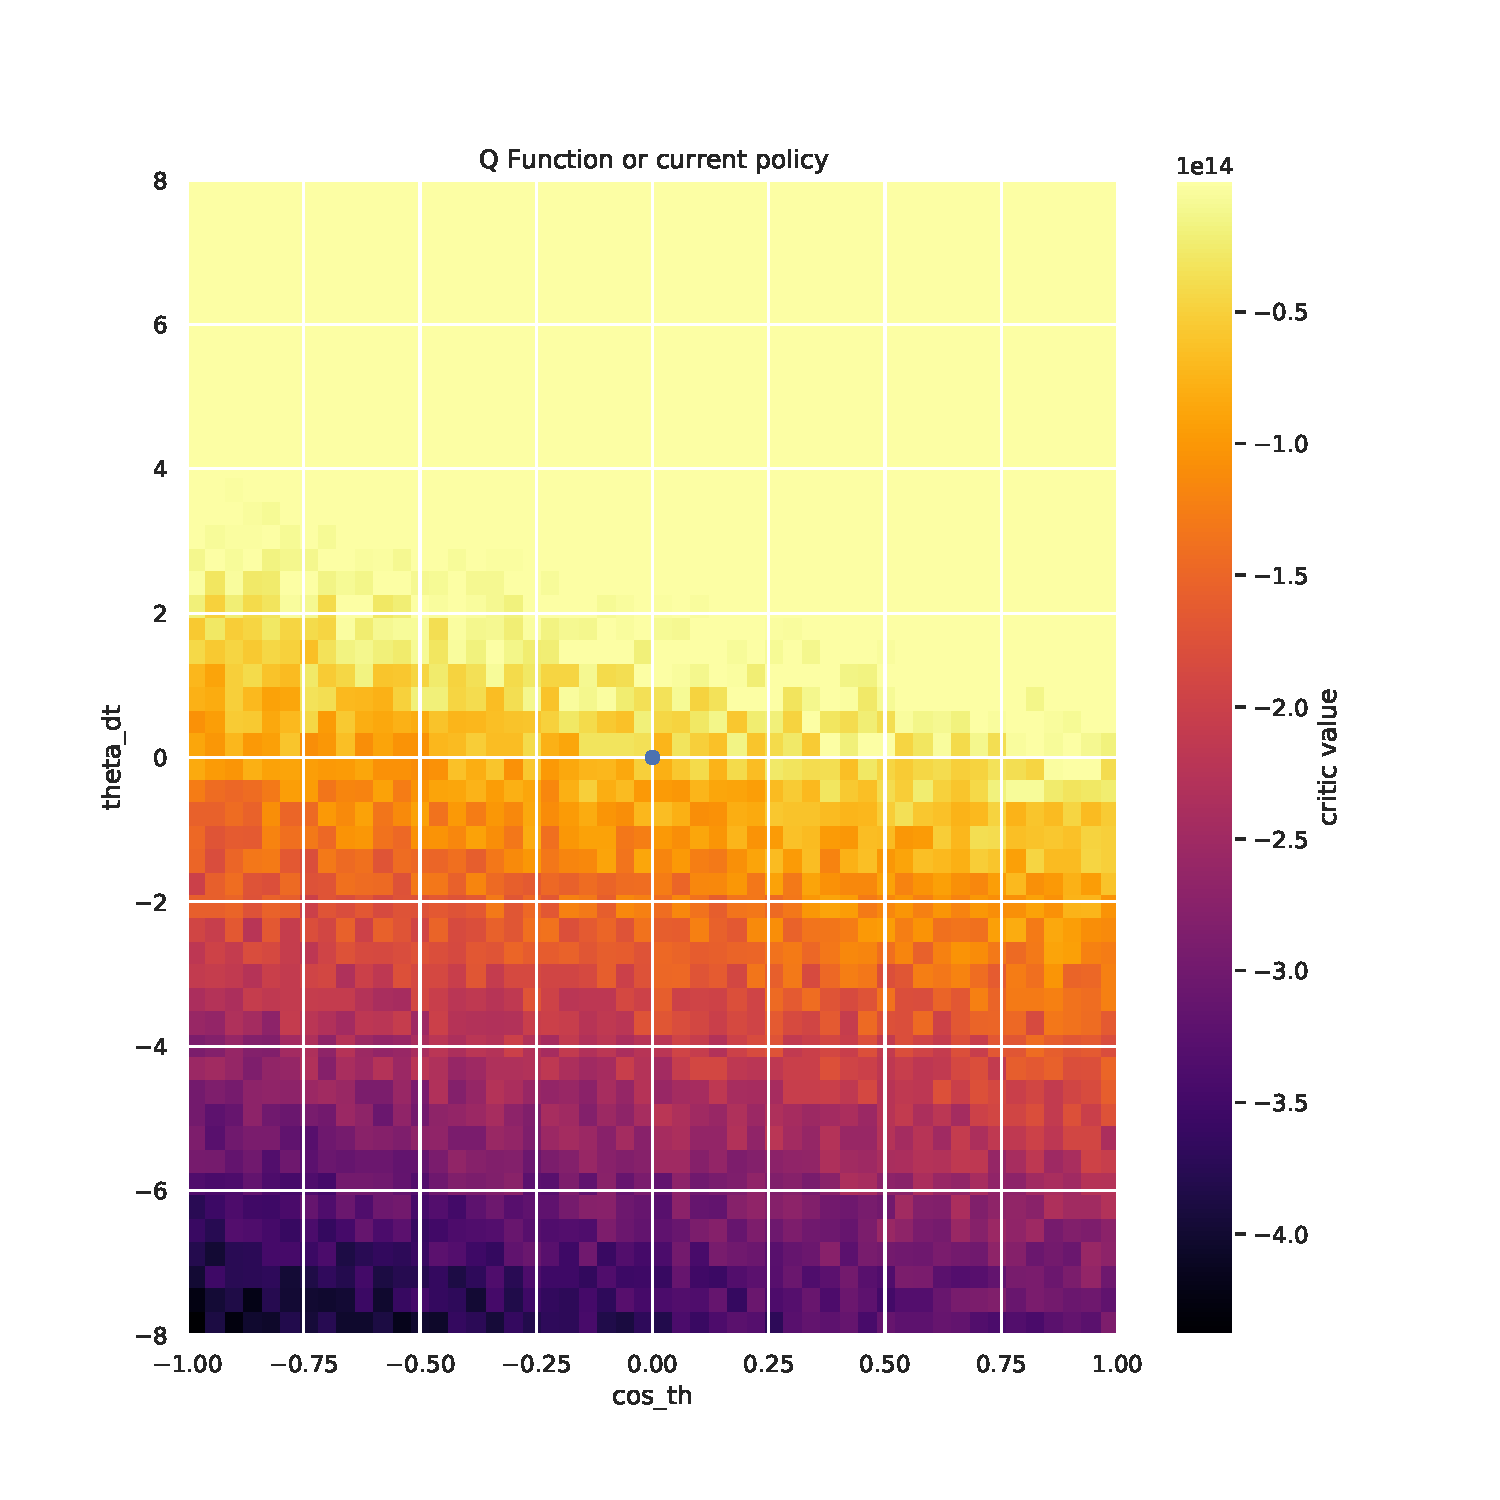
\includegraphics[width=\textwidth]{figures/iteration1/0_critic_normalize_post_Pendulum-v0.pdf}
        \caption{Critique entraînée}
    \end{subfigure}
    \caption{Valeurs de l'acteur et de la critique avec la méthode normale pour le calcul de la récompense}
    \label{fig:attempt1_normalize}
\end{figure}

Sur la figure~\ref{fig:attempt1_normalize} mis à part l'acteur naïf qui est différent parce qu'il est généré aléatoirement, l'acteur et la critique après entraînement sont identiques à ceux obtenus avec \emph{discount}. Ces résultats ne sont pas satisfaisants non plus.

\begin{figure}[H]
    \centering
    \begin{subfigure}{0.3\textwidth}
        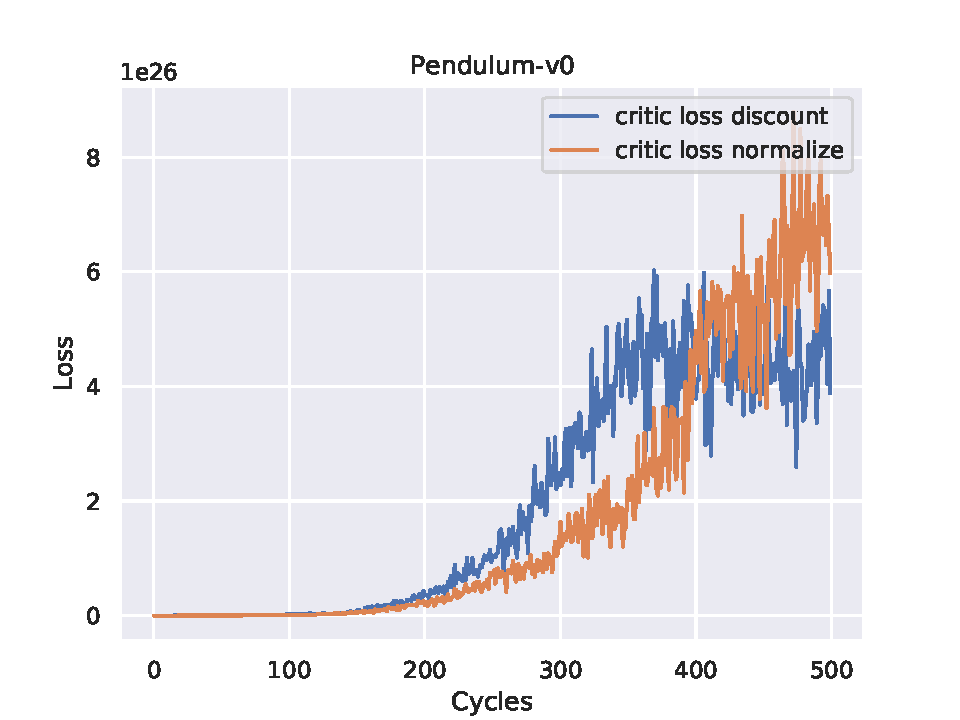
\includegraphics[width=\textwidth]{figures/iteration1/critic_loss_Pendulum-v0_pg_dataset_td_eval_True_cycles_500_trajs_20_batches_20_gamma_0.99_nstep_5_lr_act_0.01_lr_critic_0.01pg.pdf}
        \caption{Fonction de perte de la critique}
    \end{subfigure}
    \begin{subfigure}{0.3\textwidth}
        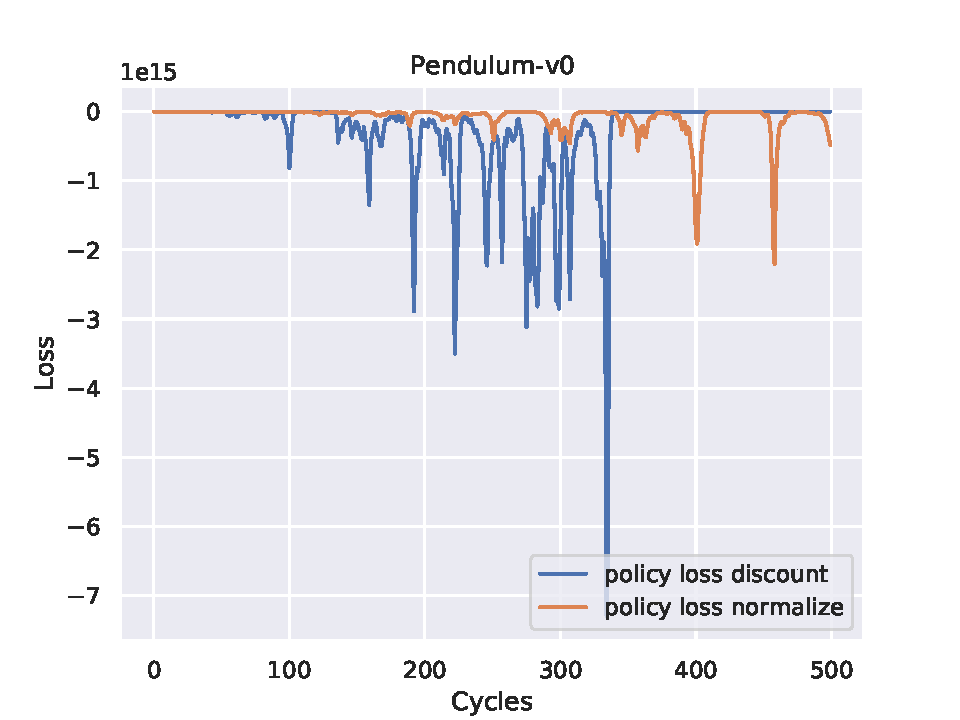
\includegraphics[width=\textwidth]{figures/iteration1/policy_loss_Pendulum-v0_pg_dataset_td_eval_True_cycles_500_trajs_20_batches_20_gamma_0.99_nstep_5_lr_act_0.01_lr_critic_0.01pg.pdf}
        \caption{Fonction de perte de la politique}
    \end{subfigure}
    \begin{subfigure}{0.3\textwidth}
        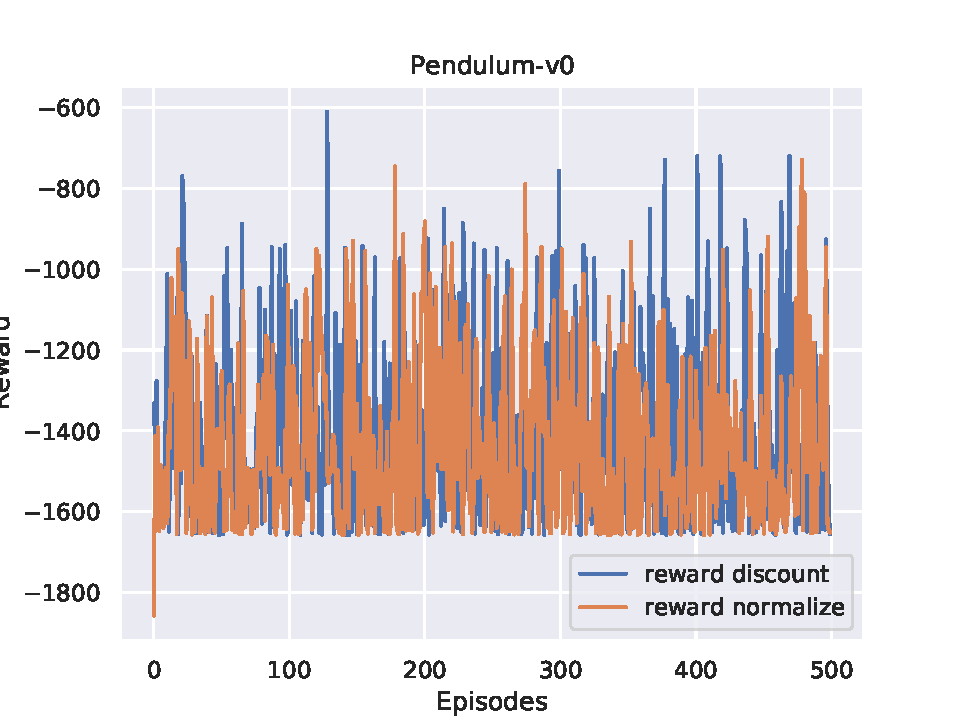
\includegraphics[width=\textwidth]{figures/iteration1/rewards_Pendulum-v0_pg_dataset_td_eval_True_cycles_500_trajs_20_batches_20_gamma_0.99_nstep_5_lr_act_0.01_lr_critic_0.01.pdf}
        \caption{Récompenses des épisodes}
    \end{subfigure}
    \caption{Résultats obtenus pour la critique, la politique et la récompense}
    \label{fig:attempt1_results}
\end{figure}

La figure~\ref{fig:attempt1_results} montre que la perte de la méthode \emph{discount} se stabilise au bout de 350 cycles tandis que celle de la méthode \emph{normalize} continu de diverger. La fonction de perte de la critique est très mauvaise avec un ordre de grandeur de $10^{15}$ pour la perte. Mais nous pouvons voir que la critique de la méthode \emph{normalize} est légèrement meilleure. Enfin la courbe des récompenses ne montre pas de convergence vers 0 que nous attendons. A contrario, il semble rester stagner au minimum, c'est à dire en bas du pendule, entre les épisodes.
\subsection{Itération n°2}

\subsubsection{Configuration et modifications}
 
 Nous décidons de redimensionner la récompense obtenue à chaque pas de temps de sorte à ce quelle soit bornée entre $0$ et $100$. À partir de l'équation~\eqref{eq:reward}, nous déterminons que $r_{min} = r(\pi, 8, 2) \simeq -45,88$ et $r_{max} = r(0, 0, 0) = 0$. Avec ces bornes nous écrivons l'inégalité~\eqref{eq:itr2_inegalite}.
 
\begin{align}
    r_{min} &< r < 0 \label{eq:itr2_inegalite} \\
    1 &> \frac{r}{r_{min}} > 0 &&\text{car $r_{min}<0$}\\
    0 &< 1 - \frac{r}{r_{min}} < 1 &&\text{par multiplication par $-1$ puis addition de $1$}\\
    0 &< 100 \times \left( 1 - \frac{r}{r_{min}} \right) < 100 \label{eq:itr2_rescale}
\end{align}
 
Nous modifions le \emph{pendulum wrapper} pour qu'il intègre le redimensionnement de l'équation~\eqref{eq:itr2_rescale}.

\subsubsection{Analyse}

\begin{figure}[H]
    \centering
    \begin{subfigure}{0.3\textwidth}
        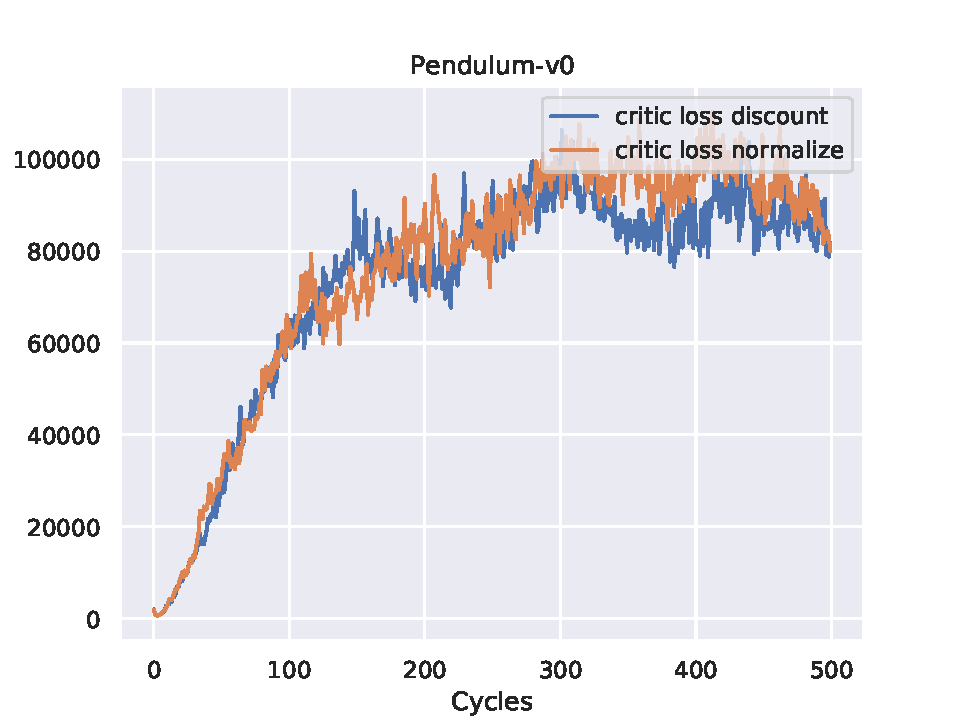
\includegraphics[width=\textwidth]{figures/iteration2/critic_loss_Pendulum-v0_pg_dataset_td_eval_True_cycles_500_trajs_20_batches_20_gamma_0.99_nstep_5_lr_act_0.01_lr_critic_0.01pg.pdf}
        \caption{Fonction de perte de la critique}
    \end{subfigure}
    \begin{subfigure}{0.3\textwidth}
        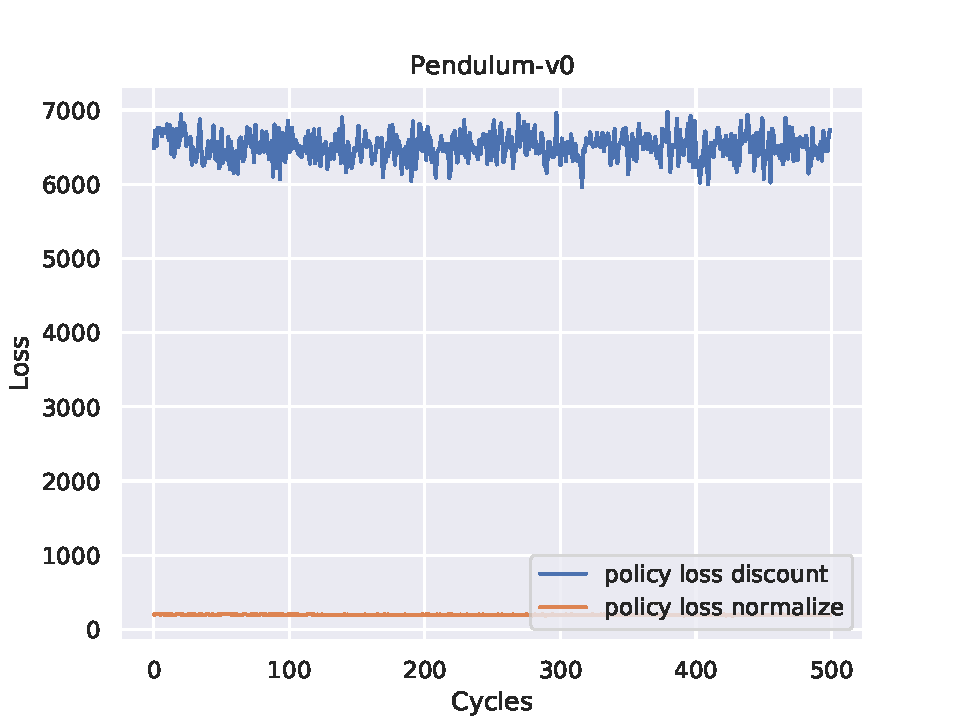
\includegraphics[width=\textwidth]{figures/iteration2/policy_loss_Pendulum-v0_pg_dataset_td_eval_True_cycles_500_trajs_20_batches_20_gamma_0.99_nstep_5_lr_act_0.01_lr_critic_0.01pg.pdf}
        \caption{Fonction de perte de la politique}
    \end{subfigure}
    \begin{subfigure}{0.3\textwidth}
        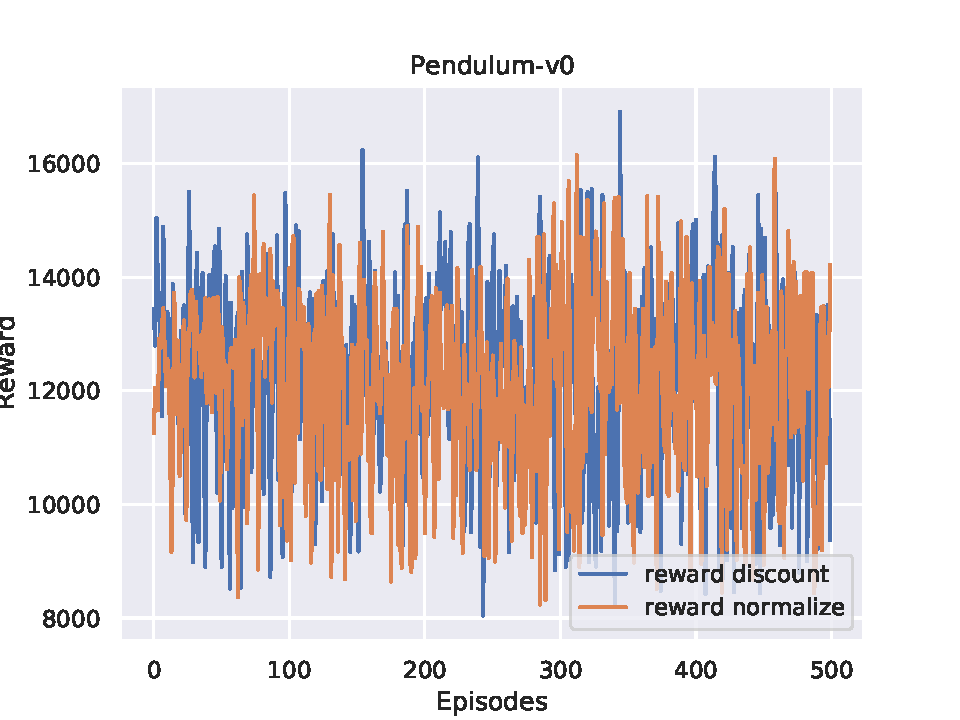
\includegraphics[width=\textwidth]{figures/iteration2/rewards_Pendulum-v0_pg_dataset_td_eval_True_cycles_500_trajs_20_batches_20_gamma_0.99_nstep_5_lr_act_0.01_lr_critic_0.01.pdf}
        \caption{Récompenses des épisodes}
    \end{subfigure}
    \caption{Résultats obtenus pour la critique, la politique et la récompense}
    \label{fig:itr2_results}
\end{figure}

Grâce au redimensionnement de la récompense, les résultats de la figure~\ref{fig:itr2_results} nous montre une convergence de la fonction de perte de la critique bien que très élevé (un peu en dessous des 100 000). On observe également que la fonction de perte est constante pour la méthode \emph{discount} et \emph{normalize}. Mais la perte de la politique obtenue par \emph{normalize} est autour de $100$ et de presque sans bruit. Tandis que celle obtenue par \emph{discount} est très bruitée et se situe autour des $6500$. On aurait donc tendance à croire que la méthode \emph{normalize} doit être favorisée dans le futur. Dans la courbe des récompenses, on n'observe plus de saturation en bas de la courbe comme dans l'itération précédente (voir fig~\ref{fig:attempt1_results}). On peut en déduire qu'il y a plus d'exploration et que le pendule reste moins souvent en bas au cours de tout un épisode.

\begin{figure}[H]
    \centering
    \begin{subfigure}{0.3\textwidth}
        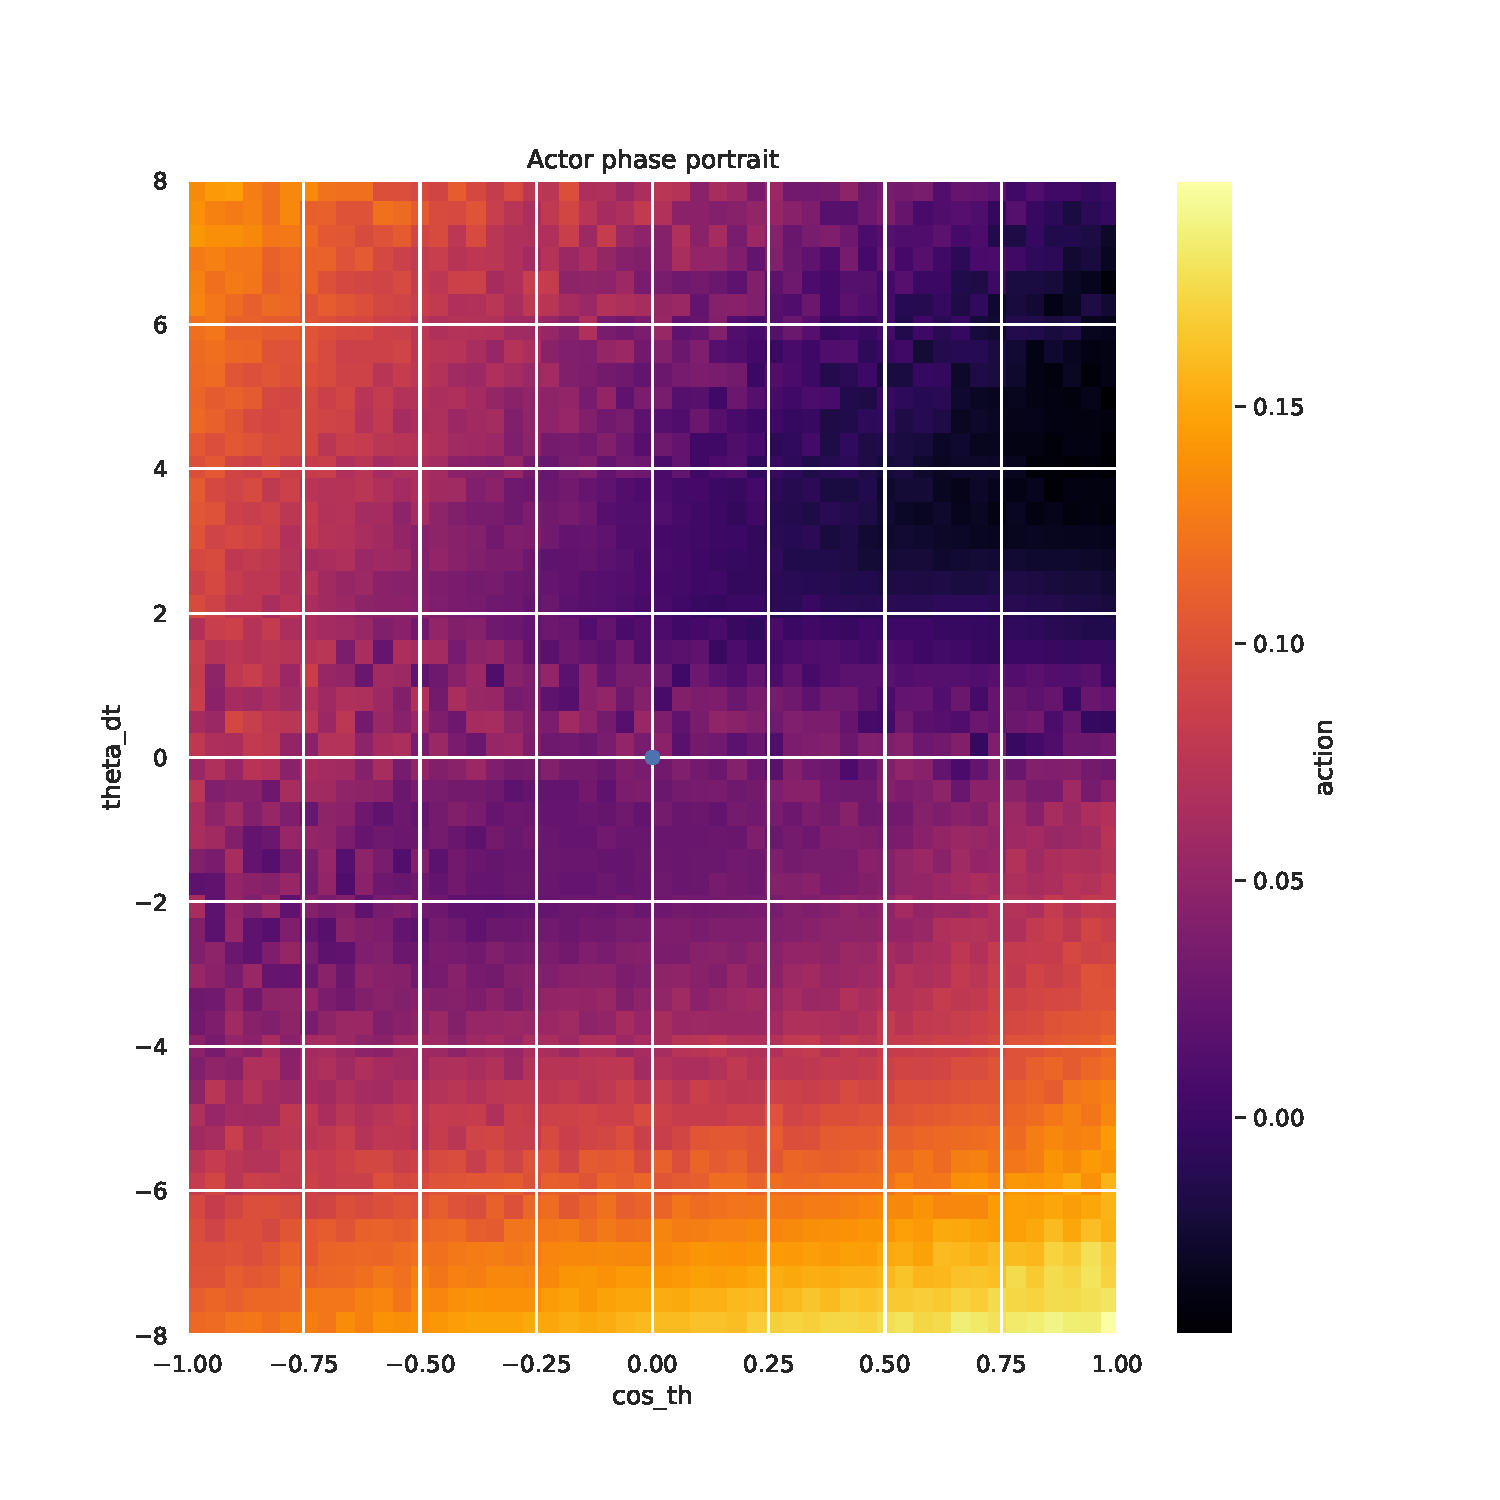
\includegraphics[width=\textwidth]{figures/iteration2/0_actor_discount__ante_Pendulum-v0.pdf}
        \caption{Acteur naïf}
    \end{subfigure}
    \begin{subfigure}{0.3\textwidth}
        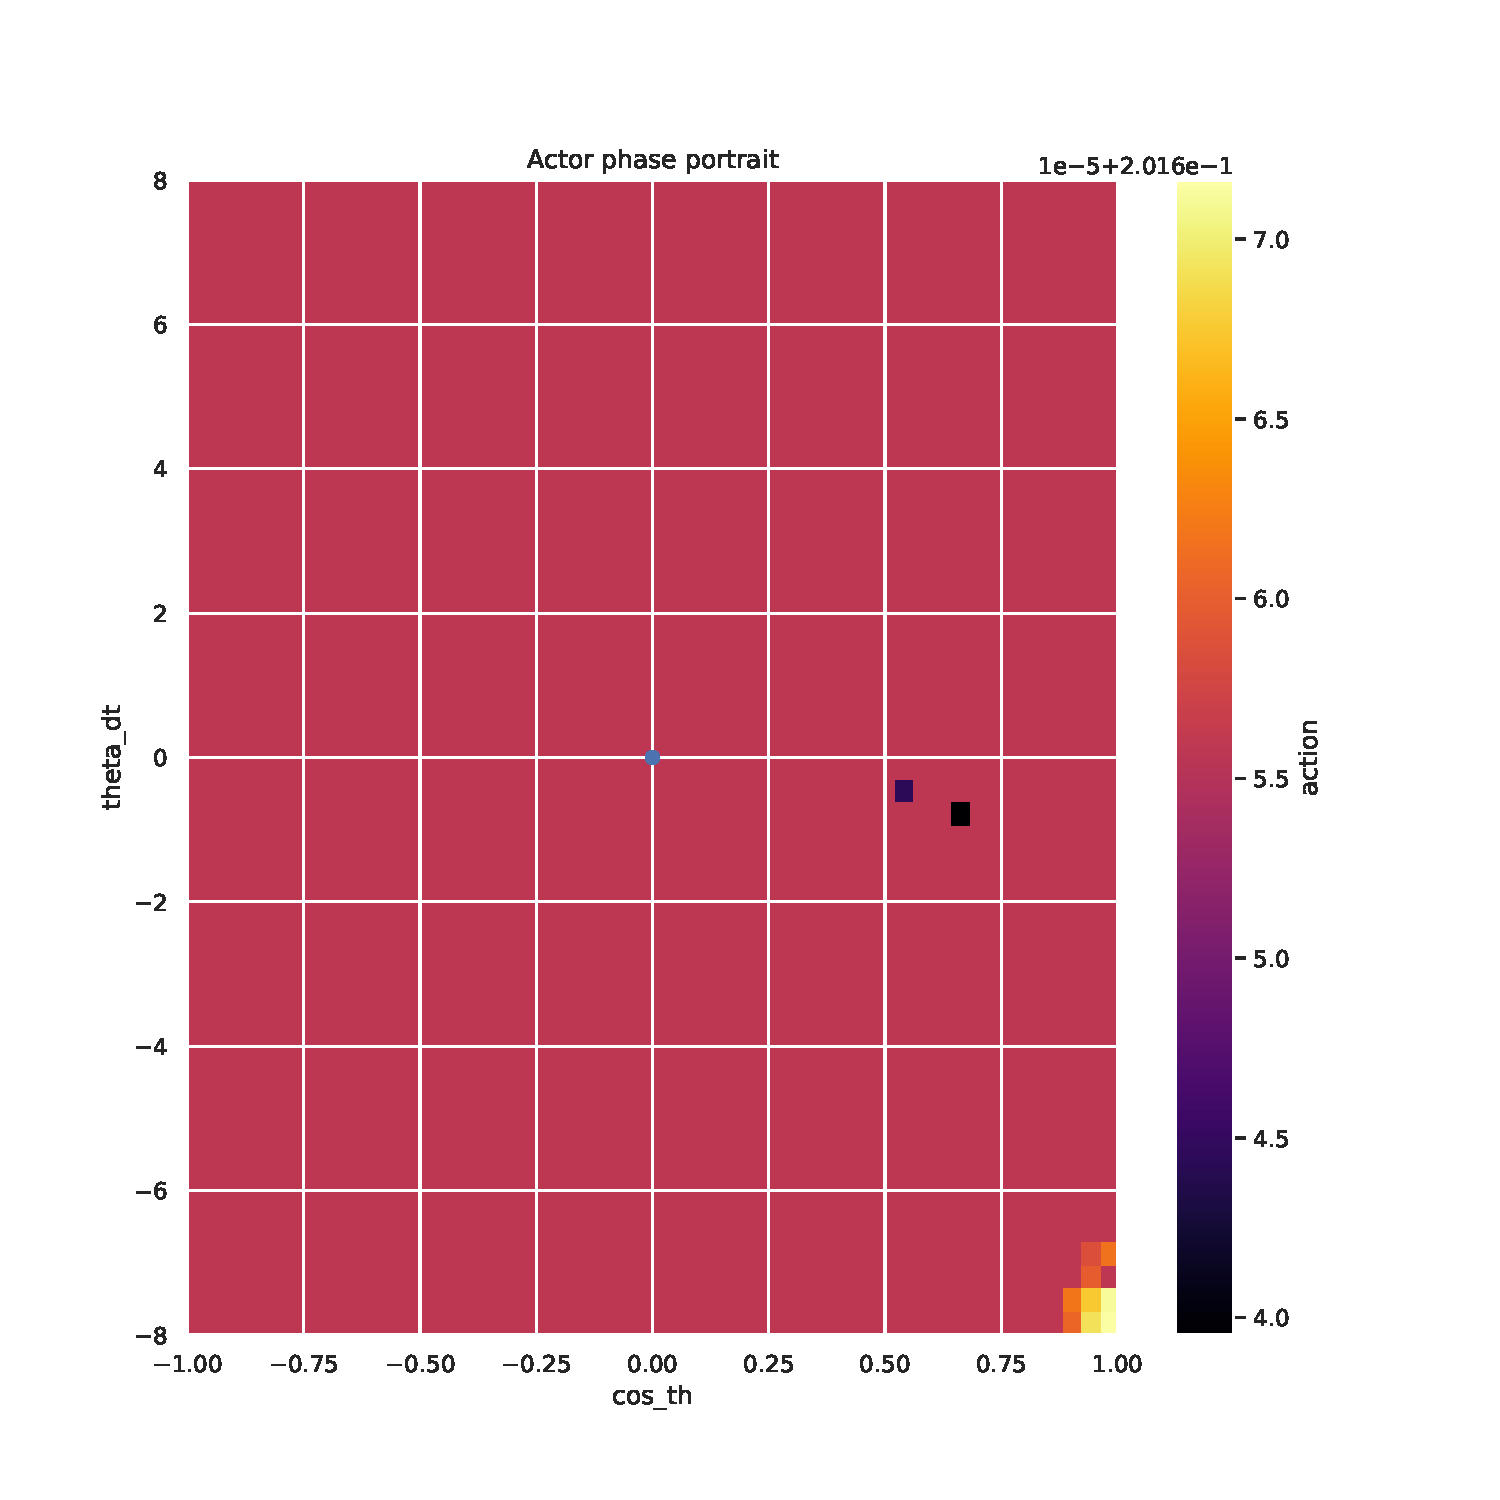
\includegraphics[width=\textwidth]{figures/iteration2/0_actor_discount__post_Pendulum-v0.pdf}
        \caption{Acteur entraîné}
    \end{subfigure}
    \begin{subfigure}{0.3\textwidth}
        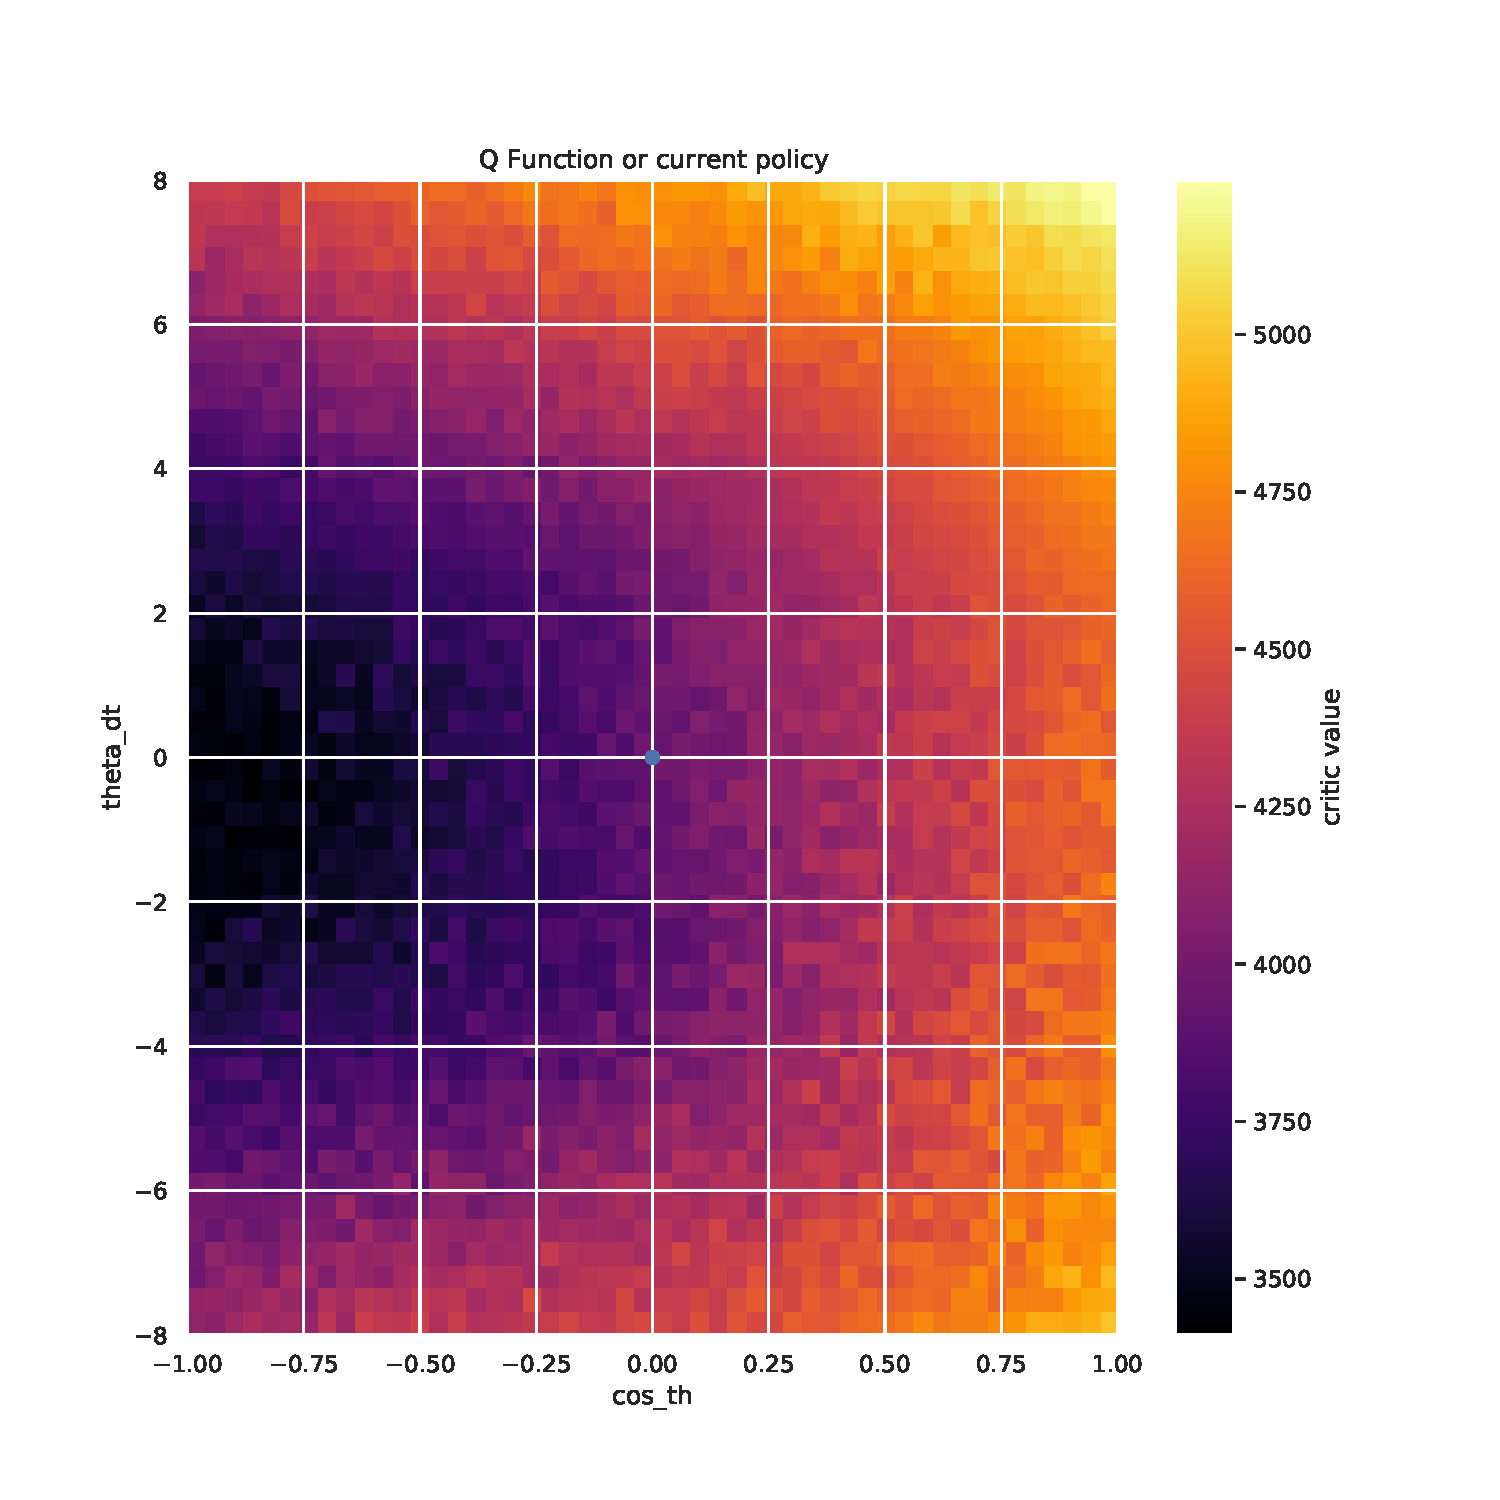
\includegraphics[width=\textwidth]{figures/iteration2/0_critic_discount_post_Pendulum-v0.pdf}
        \caption{Critique entraînée}
    \end{subfigure}
    \caption{Valeurs de l'acteur et de la critique avec la méthode discount pour le calcul de la récompense}
    \label{fig:itr2_discount}
\end{figure}

Dans la figure~\ref{fig:itr2_discount} on retrouve l'acteur uniforme sur l'ensemble des états. De plus, nous ne comprenons pas l'ordre de grandeur de l'échelle des actions. Concernant la critique, elle ne correspond pas à ce qu'on attend car les points clairs sont pour des vitesses angulaires élevées (positive et négative) pour $\cos(\theta) = 1$ alors qu'on voudrait à cette position une vitesse nulle. 

\begin{figure}[H]
    \centering
    \begin{subfigure}{0.3\textwidth}
        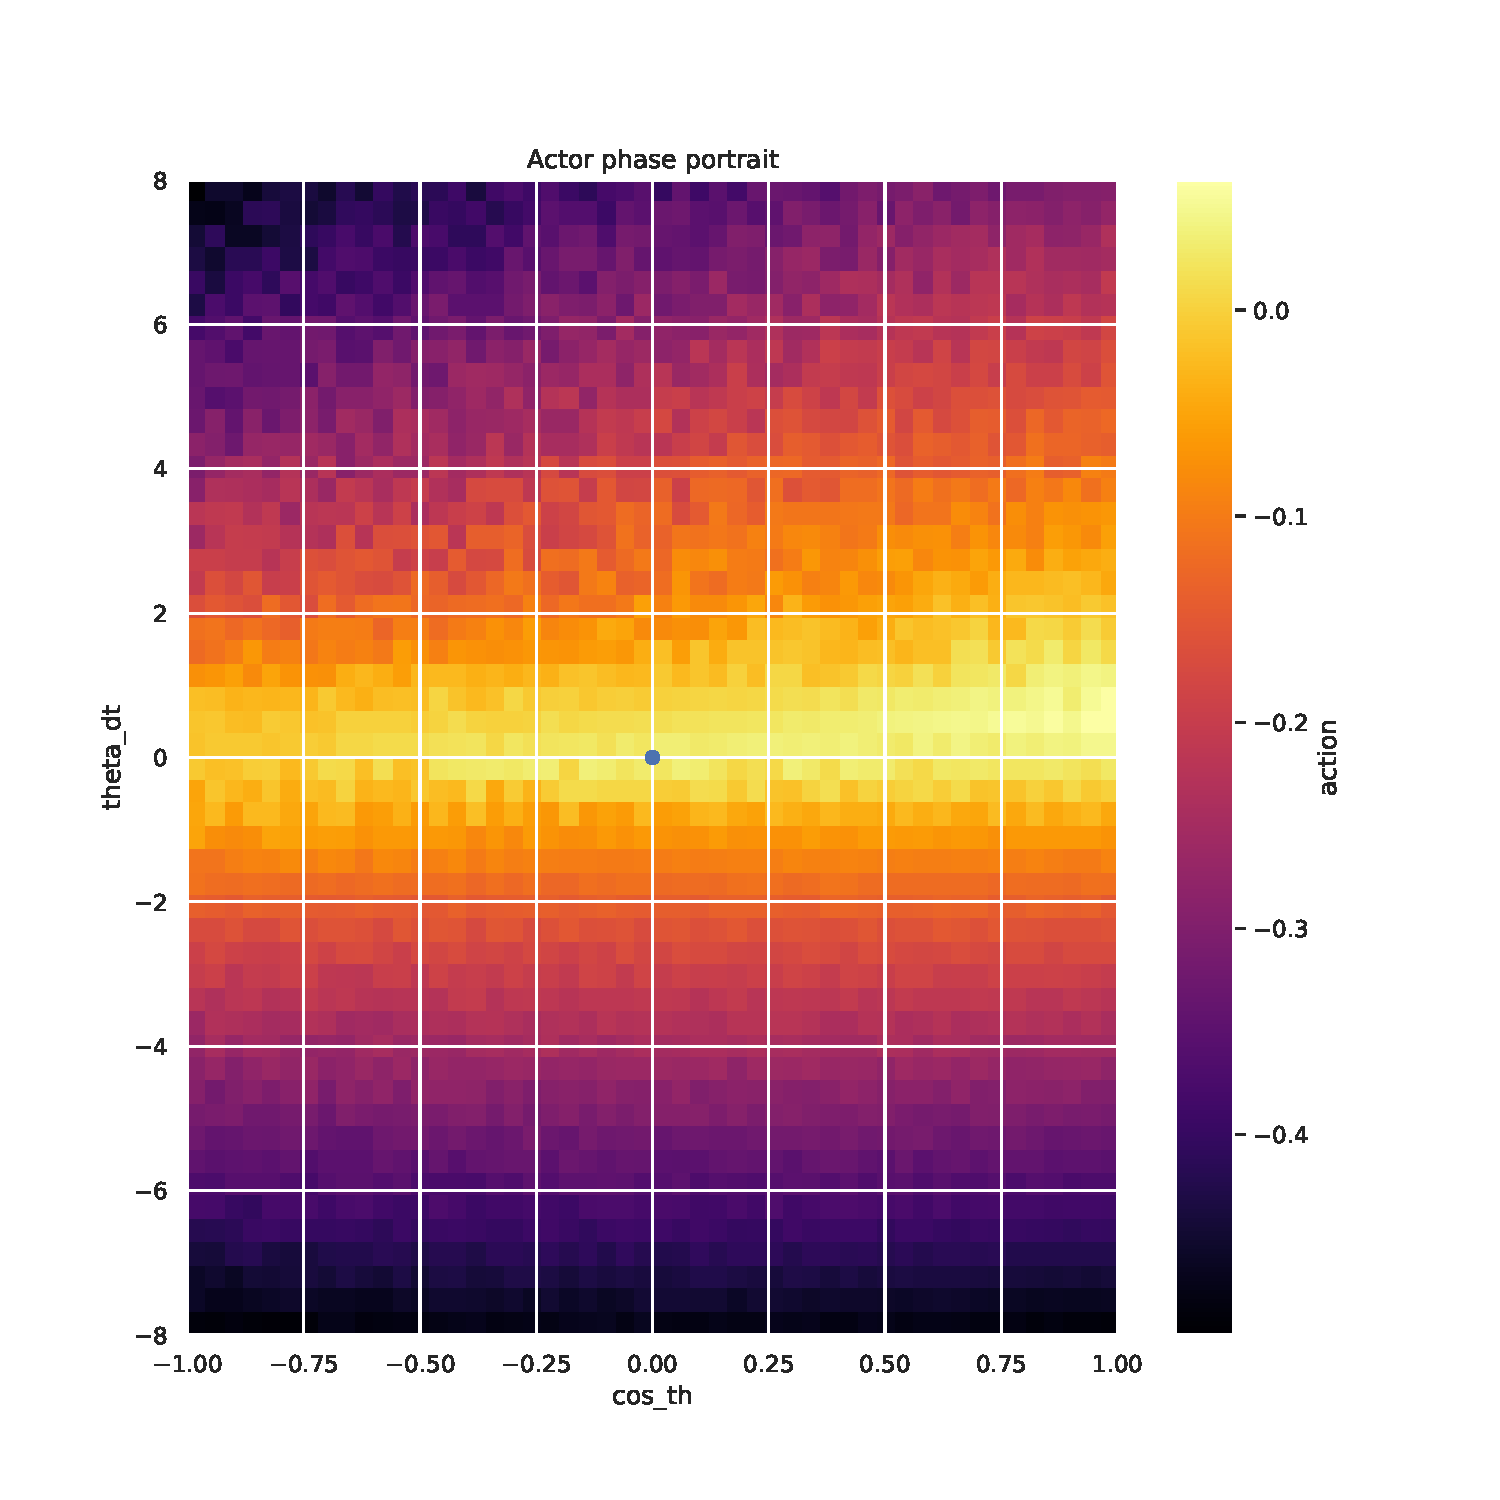
\includegraphics[width=\textwidth]{figures/iteration2/0_actor_normalize__ante_Pendulum-v0.pdf}
        \caption{Acteur naïf}
    \end{subfigure}
    \begin{subfigure}{0.3\textwidth}
        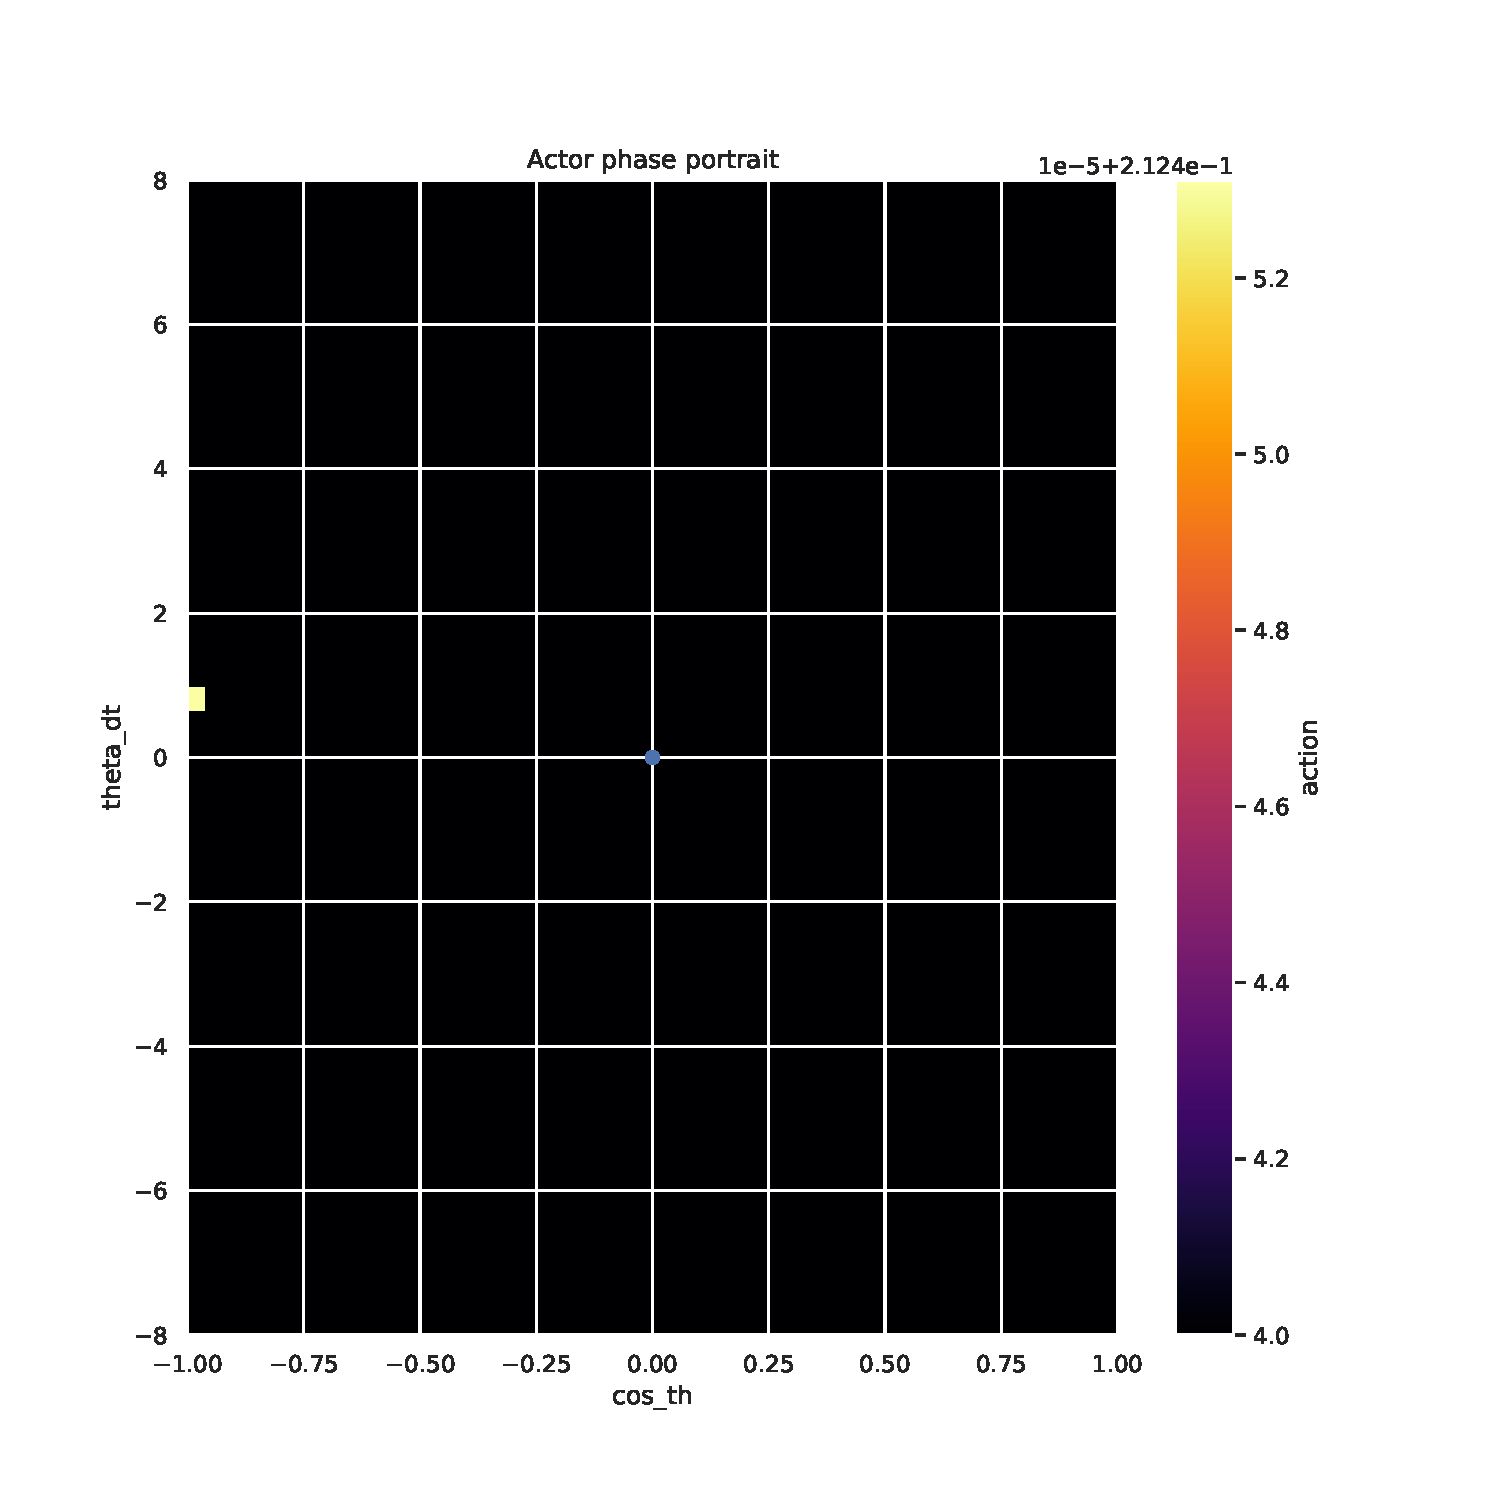
\includegraphics[width=\textwidth]{figures/iteration2/0_actor_normalize__post_Pendulum-v0.pdf}
        \caption{Acteur entraîné}
    \end{subfigure}
    \begin{subfigure}{0.3\textwidth}
        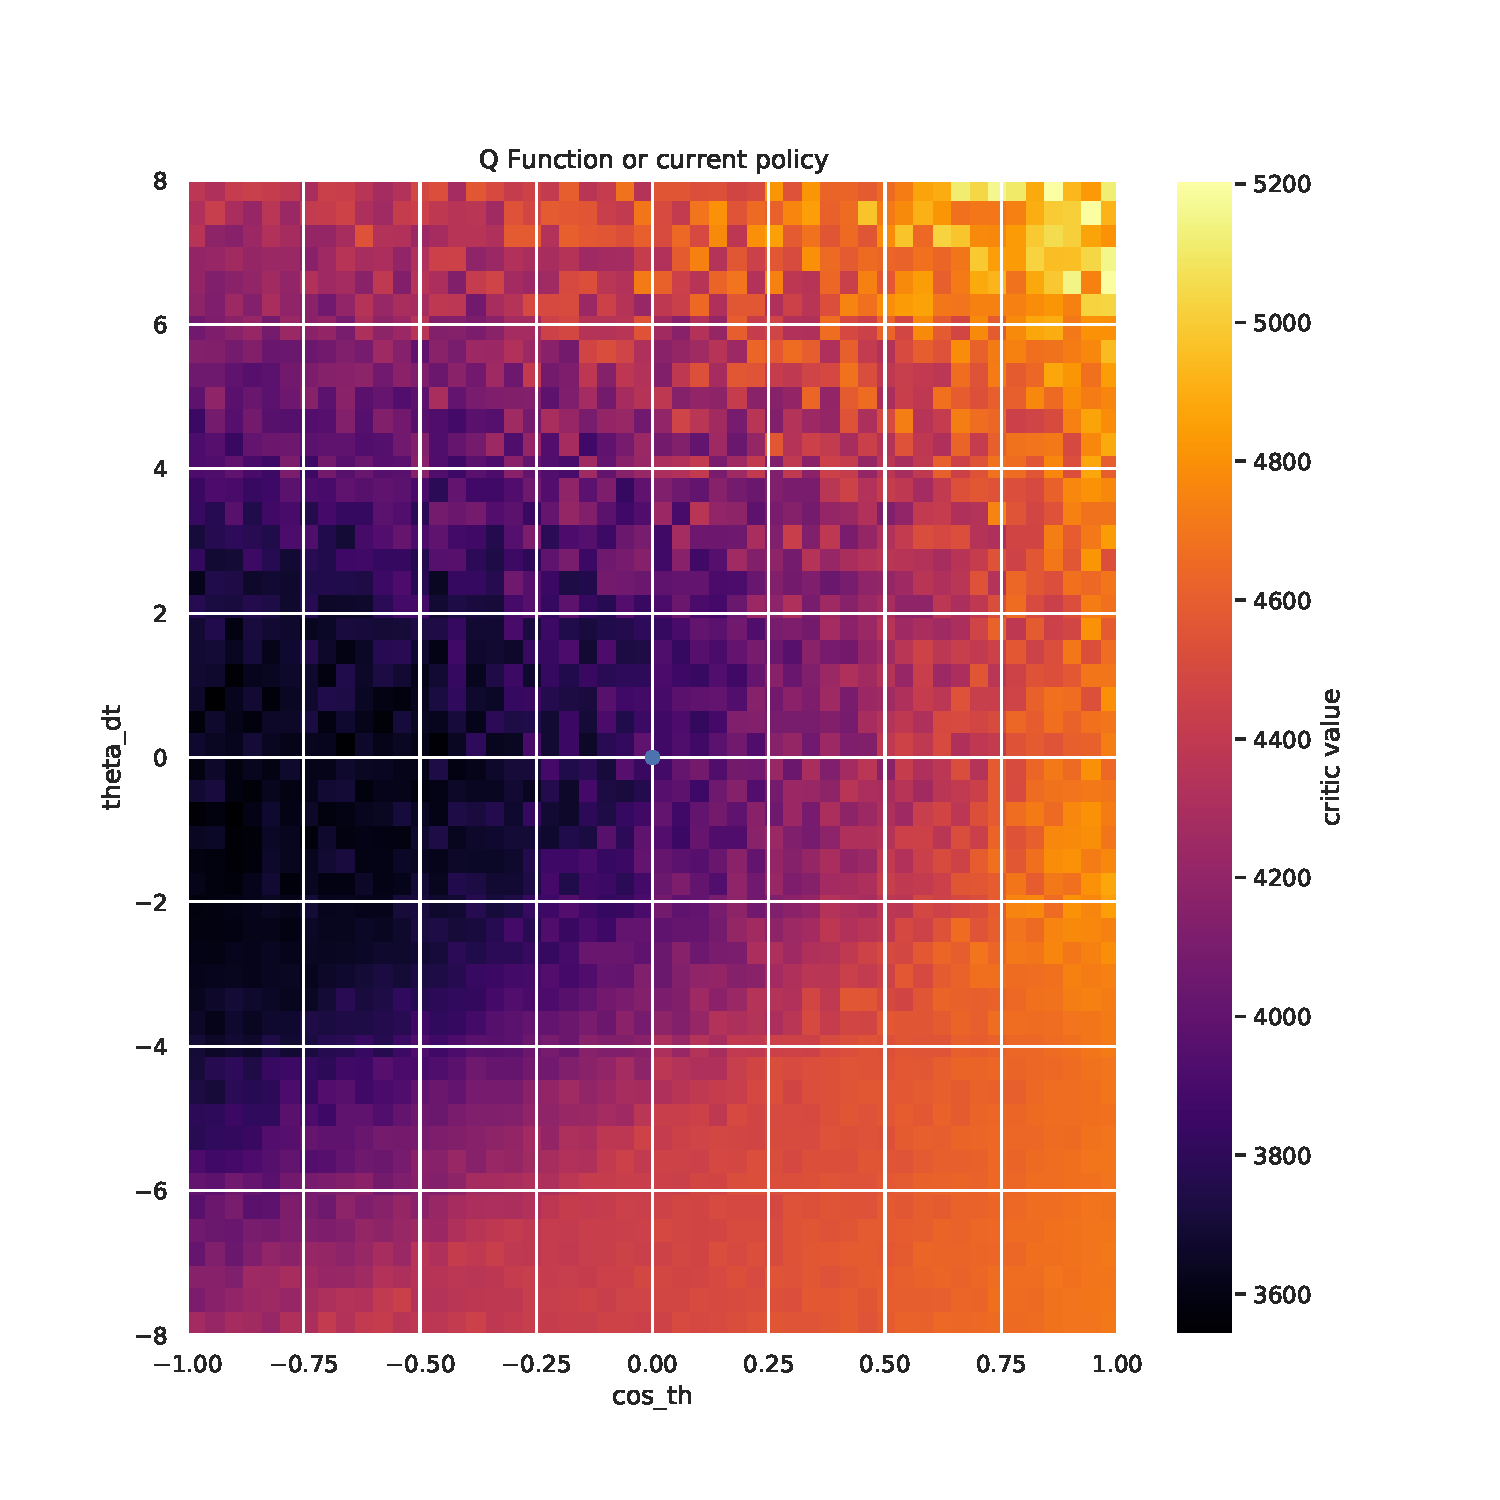
\includegraphics[width=\textwidth]{figures/iteration2/0_critic_normalize_post_Pendulum-v0.pdf}
        \caption{Critique entraînée}
    \end{subfigure}
    \caption{Valeurs de l'acteur et de la critique avec la méthode normalize pour le calcul de la récompense}
    \label{fig:itr2_normalize}
\end{figure}

Ici encore avec la figure~\ref{fig:itr2_normalize} l'acteur entraîné est encore uniforme mais aussi avec un ordre de grandeur incompréhensible sur l'échelle des actions. Comme avec la méthode \emph{discount}, la critique obtenue après apprentissage n'est pas ce que l'on souhaite. Mais pour $\cos(\theta) = -1$ et $\dot{\theta} = 0$ on a bien une zone défavorisée. On peut ainsi comprendre que le pendule évite d'être immobile en bas. Mais pour $\cos(\theta) = 1$ la vitesse à laquelle il se trouve lui importe peu bien qu'il est une préférence pour la vitesse maximale.
\subsection{Itération n°3}

\subsubsection{Configuration, modifications et résultats attendus}

Nous redimensionnons la récompense à nouveau de sorte à ce que la récompense sur un épisode soit compris entre $0$ et $100$. En faisant cela, nous souhaitons réduire l'amplitude de la récompense et le bruit associé. En réduisant le bruit, le gradient converge plus facilement vers un minimum.

Pour borner la récompense sur un épisode entre $0$ et $100$, nous divisons l'équation~\ref{eq:itr2_rescale} par le nombre de pas par épisode soit $200$.

Nous attendons à avoir une récompense par épisode bornée par $0$ et par $100$. Par la réduction d'échelle, nous attendons à obtenir une courbe moins bruitée et croissante. En effet, la réduction du bruit permet une variation plus fine des poids et des biais.  Donc avoir une évolution plus douce. Celle-ci permet de converger vers un minimum ce qui améliore la politique et par conséquent la récompense.

\subsubsection{Analyse}

\begin{figure}[H]
    \centering
    \begin{subfigure}{0.3\textwidth}
        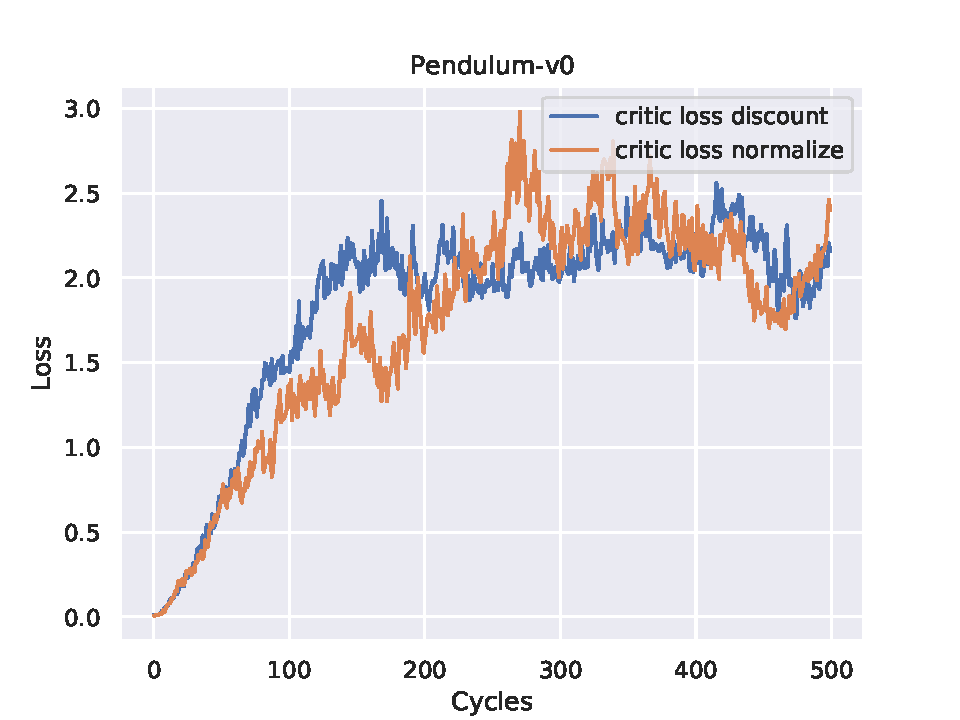
\includegraphics[width=\textwidth]{figures/iteration3/critic_loss_Pendulum-v0_pg_dataset_td_eval_True_cycles_500_trajs_20_batches_20_gamma_0.99_nstep_5_l.pdf}
        \caption{Fonction de perte de la critique}
    \end{subfigure}
    \begin{subfigure}{0.3\textwidth}
        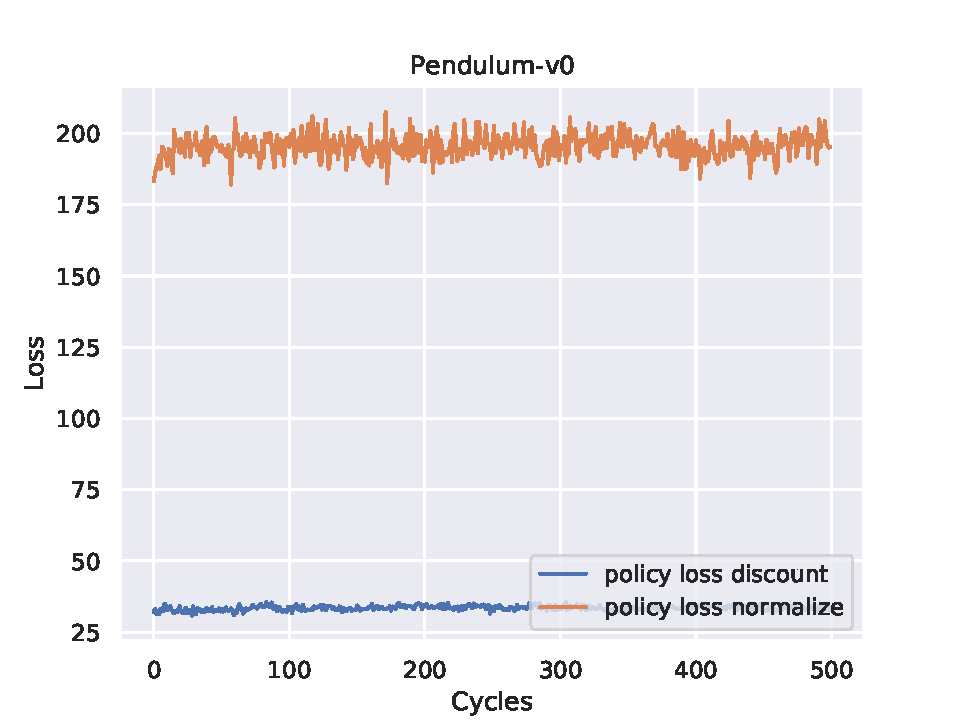
\includegraphics[width=\textwidth]{figures/iteration3/policy_loss_Pendulum-v0_pg_dataset_td_eval_True_cycles_500_trajs_20_batches_20_gamma_0.99_nstep_5_l.pdf}
        \caption{Fonction de perte de la politique}
    \end{subfigure}
    \begin{subfigure}{0.3\textwidth}
        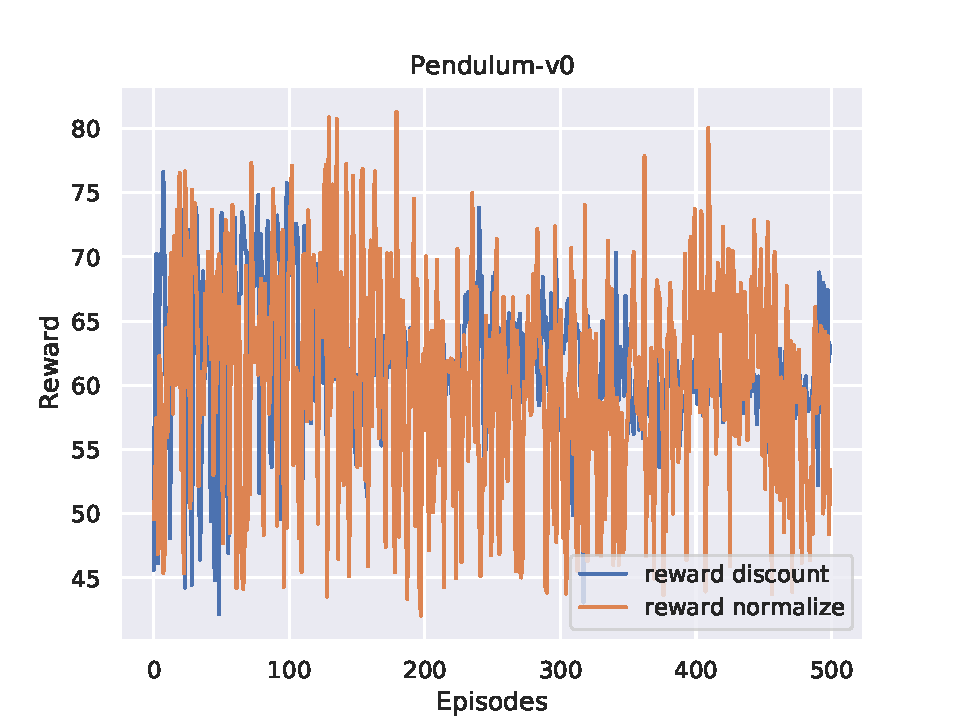
\includegraphics[width=\textwidth]{figures/iteration3/rewards_Pendulum-v0_pg_dataset_td_eval_True_cycles_500_trajs_20_batches_20_gamma_0.99_nstep_5_lr_ac.pdf}
        \caption{Récompenses des épisodes}
    \end{subfigure}
    \caption{Résultats obtenus pour la critique, la politique et la récompense}
    \label{fig:itr3_results}
\end{figure}

Nous observons que notre récompense est bien bornée entre 0 et 100 mais ne croît pas comme espéré. La récompense obtenue par la méthode \emph{discount} semble même se stabiliser aux alentours de 60.

Nous observons que la fonction de perte de la politique est relativement constante. Ce résultat est tout à fait singulier. Nous en déduisons qu'il y a un problème dans l'apprentissage de la politique. Malheureusement, nous ne somme pas parvenu à identifier le problème.

Comme précédemment, la fonction de perte de la critique ne décroît pas.

\begin{figure}[H]
    \centering
    \begin{subfigure}{0.3\textwidth}
        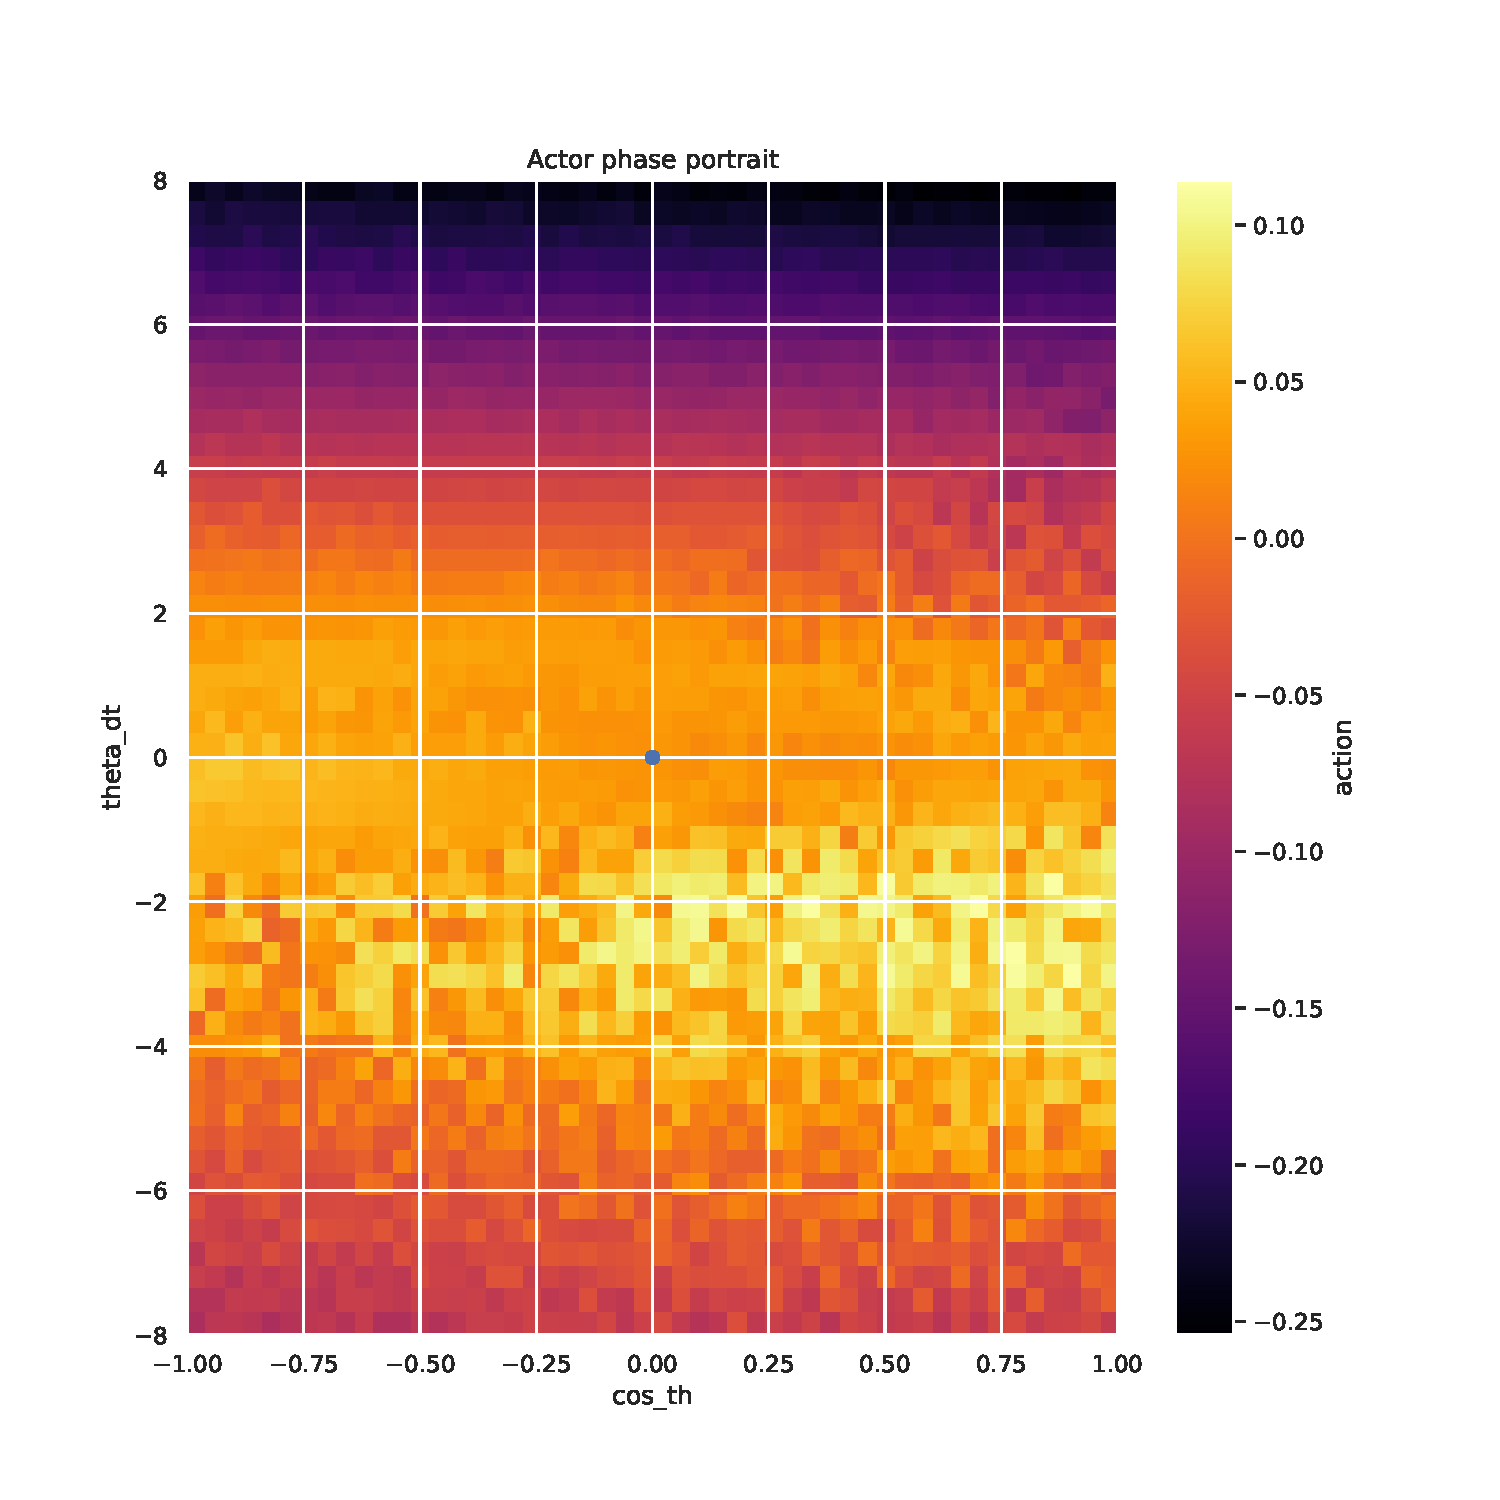
\includegraphics[width=\textwidth]{figures/iteration3/0_actor_discount__ante_Pendulum-v0.pdf}
        \caption{Acteur naïf}
    \end{subfigure}
    \begin{subfigure}{0.3\textwidth}
        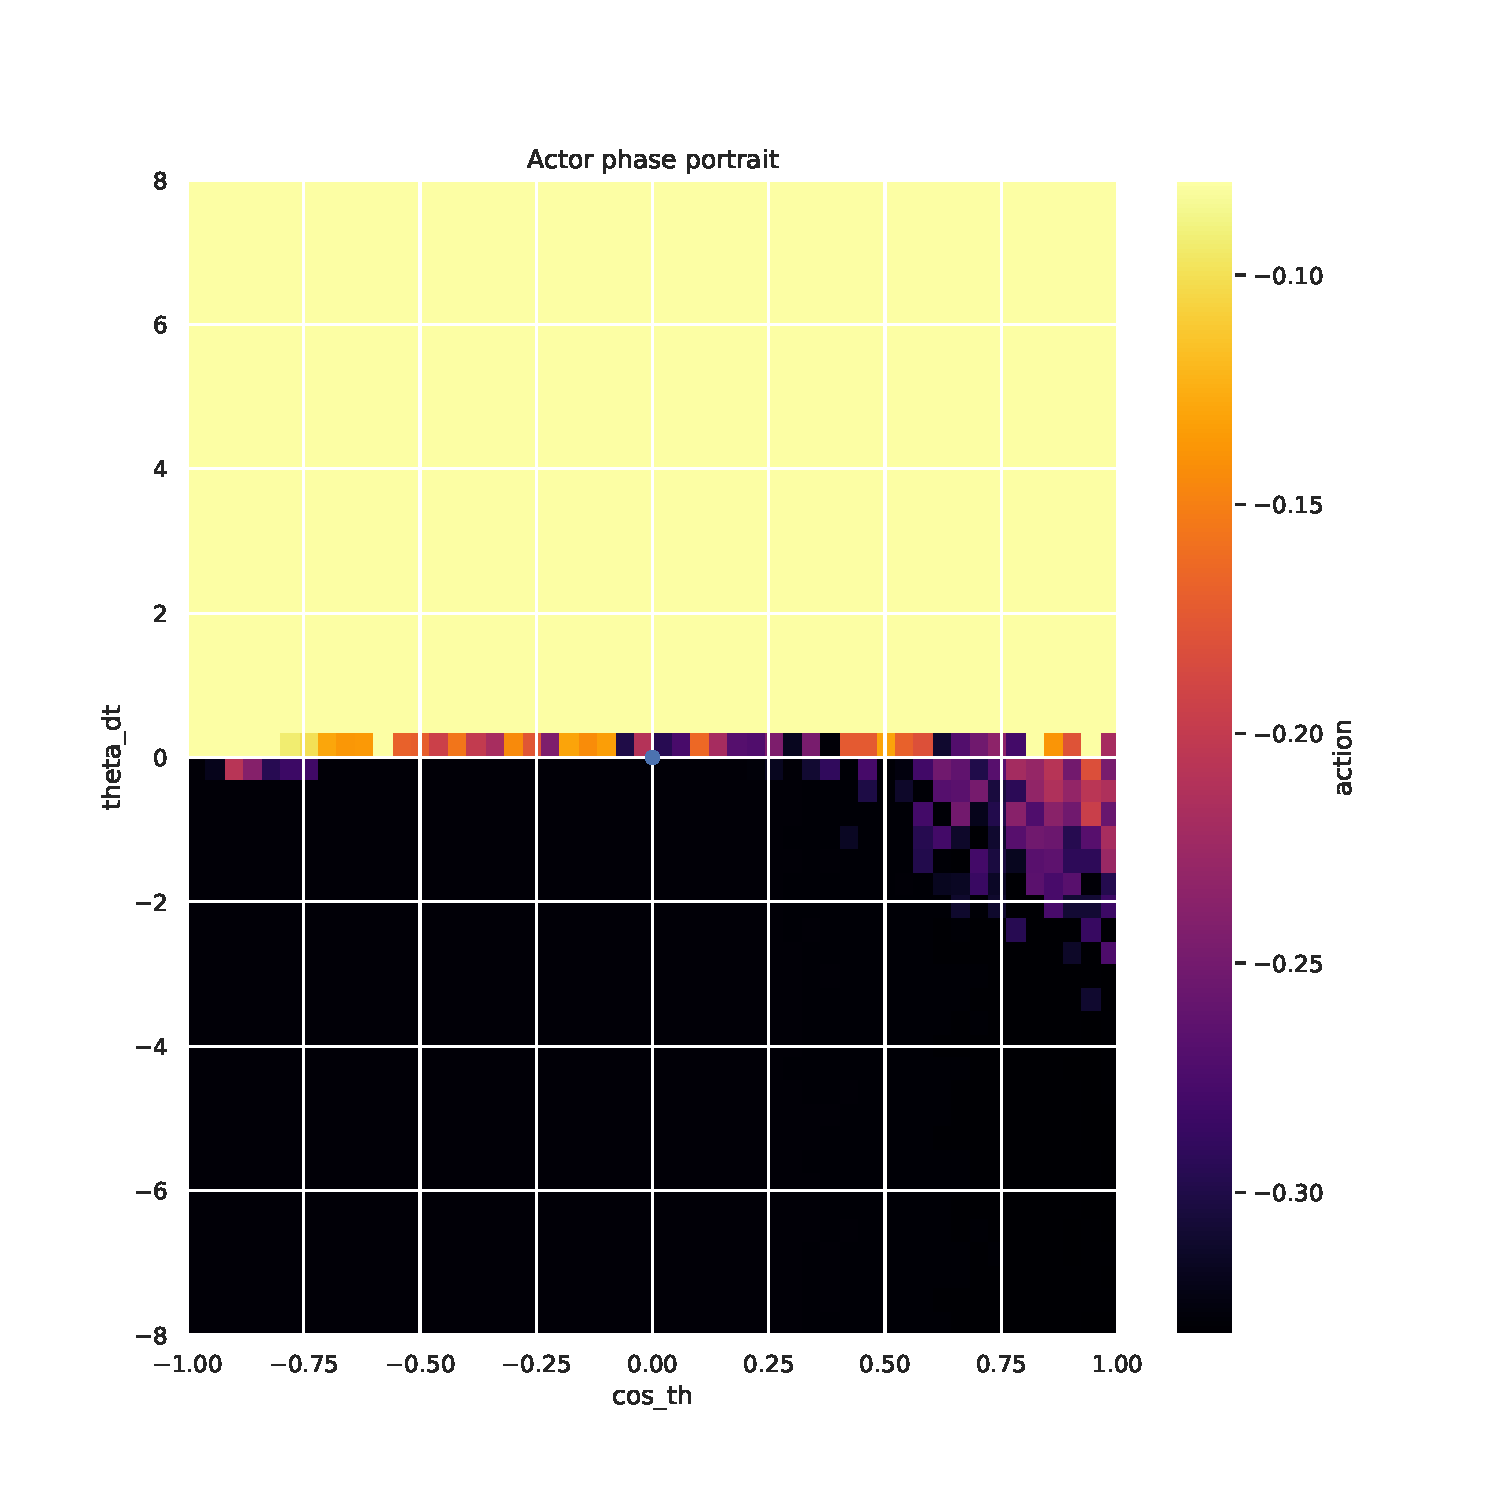
\includegraphics[width=\textwidth]{figures/iteration3/0_actor_discount__post_Pendulum-v0.pdf}
        \caption{Acteur entraîné}
    \end{subfigure}
    \begin{subfigure}{0.3\textwidth}
        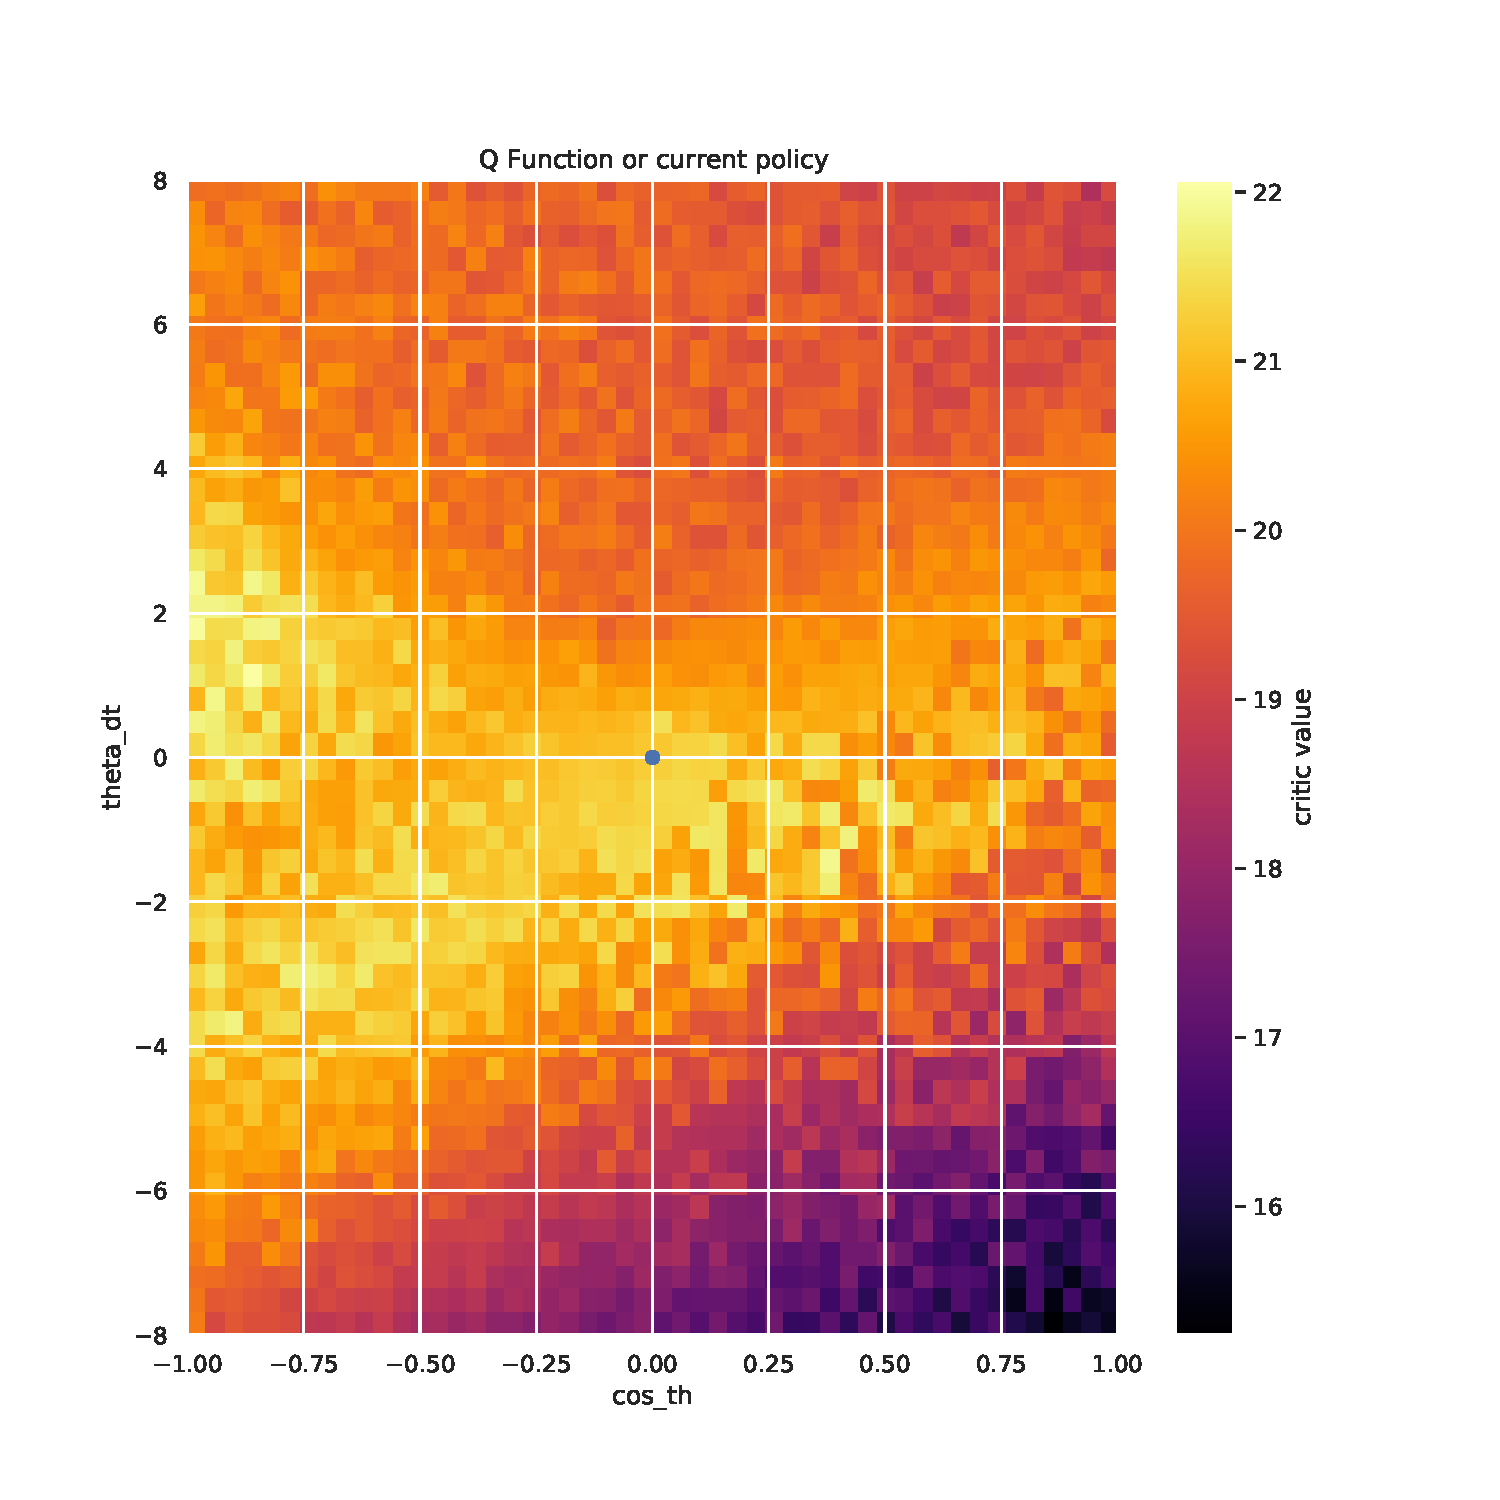
\includegraphics[width=\textwidth]{figures/iteration3/0_critic_discount_post_Pendulum-v0.pdf}
        \caption{Critique entraînée}
    \end{subfigure}
    \caption{Valeurs de l'acteur et de la critique avec la méthode discount pour le calcul de la récompense}
    \label{fig:itr3_discount}
\end{figure}

La plage d'action de l'acteur n'est pas cohérente avec ce que l'on attend. nous préférerions une plage d'action comprise entre $-2$ et $2$. L'apprentissage est définitivement mauvais car où qu'il soit et peu importe sa vitesse, il continuera de tourner.

La critique n'est toujours pas intéressante au vu de ses zones de préférence sur l'ensemble de l'intervalle de $\cos(\theta)$. De plus, la critique semble aussi favoriser la position en bas du pendule avec une vitesse faible qui ne lui fera pas quitter cet état pourtant à éviter.

\begin{figure}[H]
    \centering
    \begin{subfigure}{0.3\textwidth}
        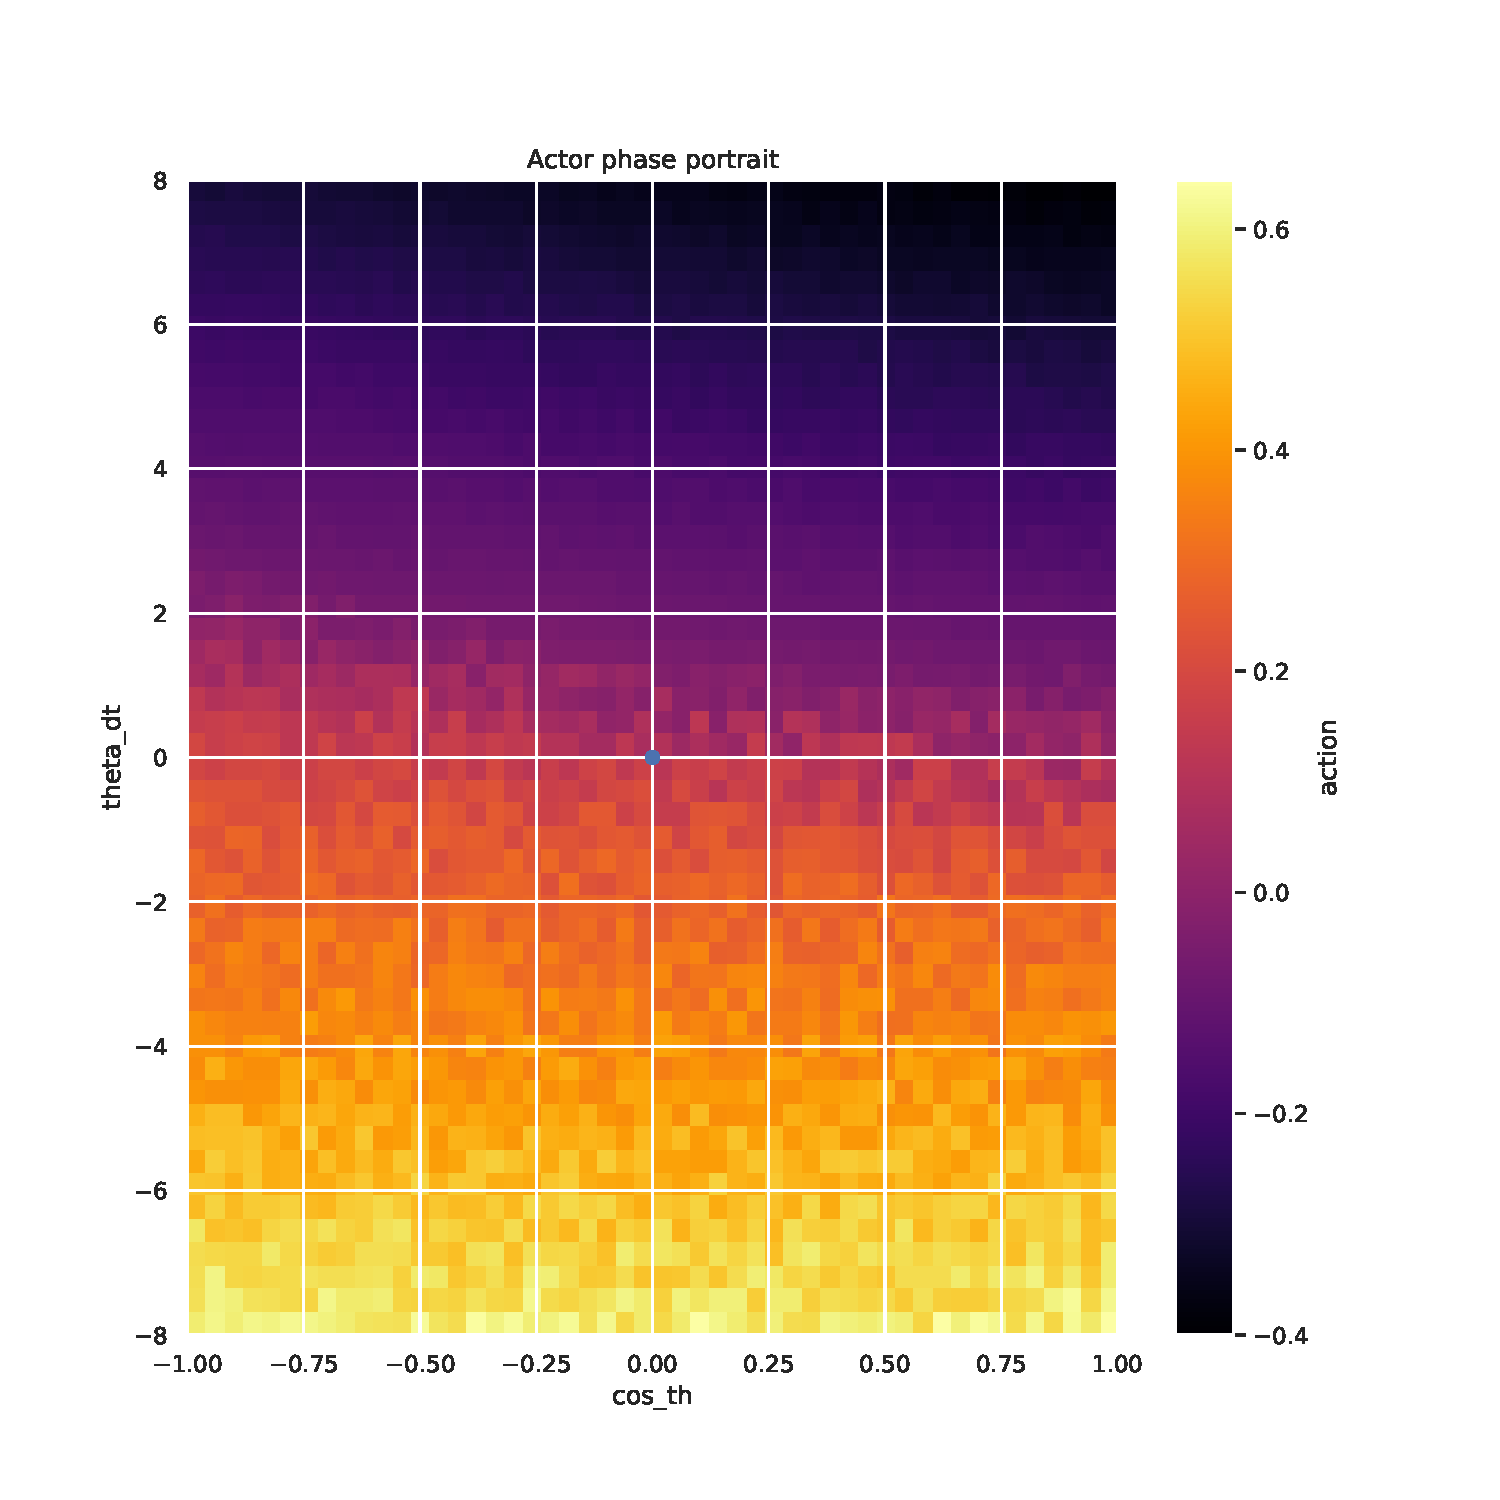
\includegraphics[width=\textwidth]{figures/iteration3/0_actor_normalize__ante_Pendulum-v0.pdf}
        \caption{Acteur naïf}
    \end{subfigure}
    \begin{subfigure}{0.3\textwidth}
        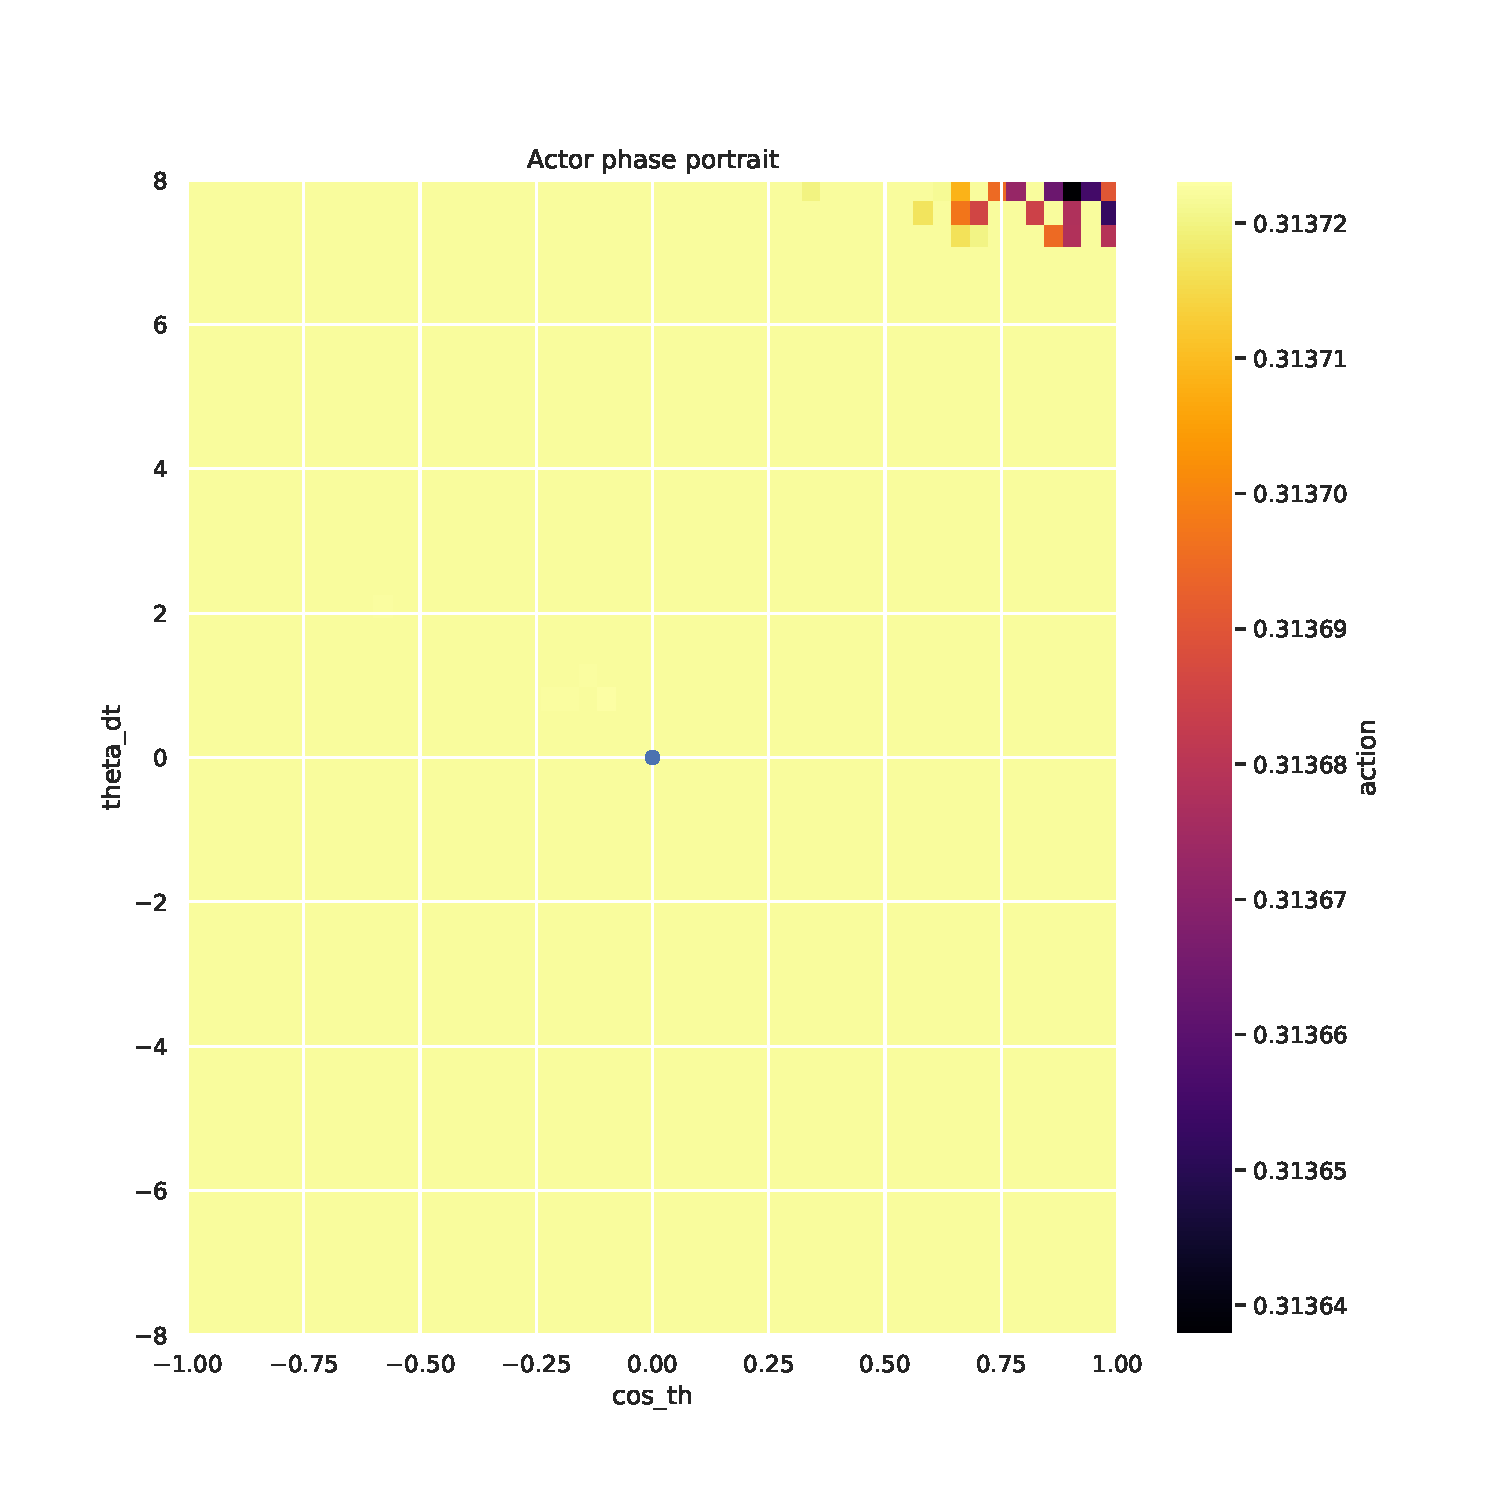
\includegraphics[width=\textwidth]{figures/iteration3/0_actor_normalize__post_Pendulum-v0.pdf}
        \caption{Acteur entraîné}
    \end{subfigure}
    \begin{subfigure}{0.3\textwidth}
        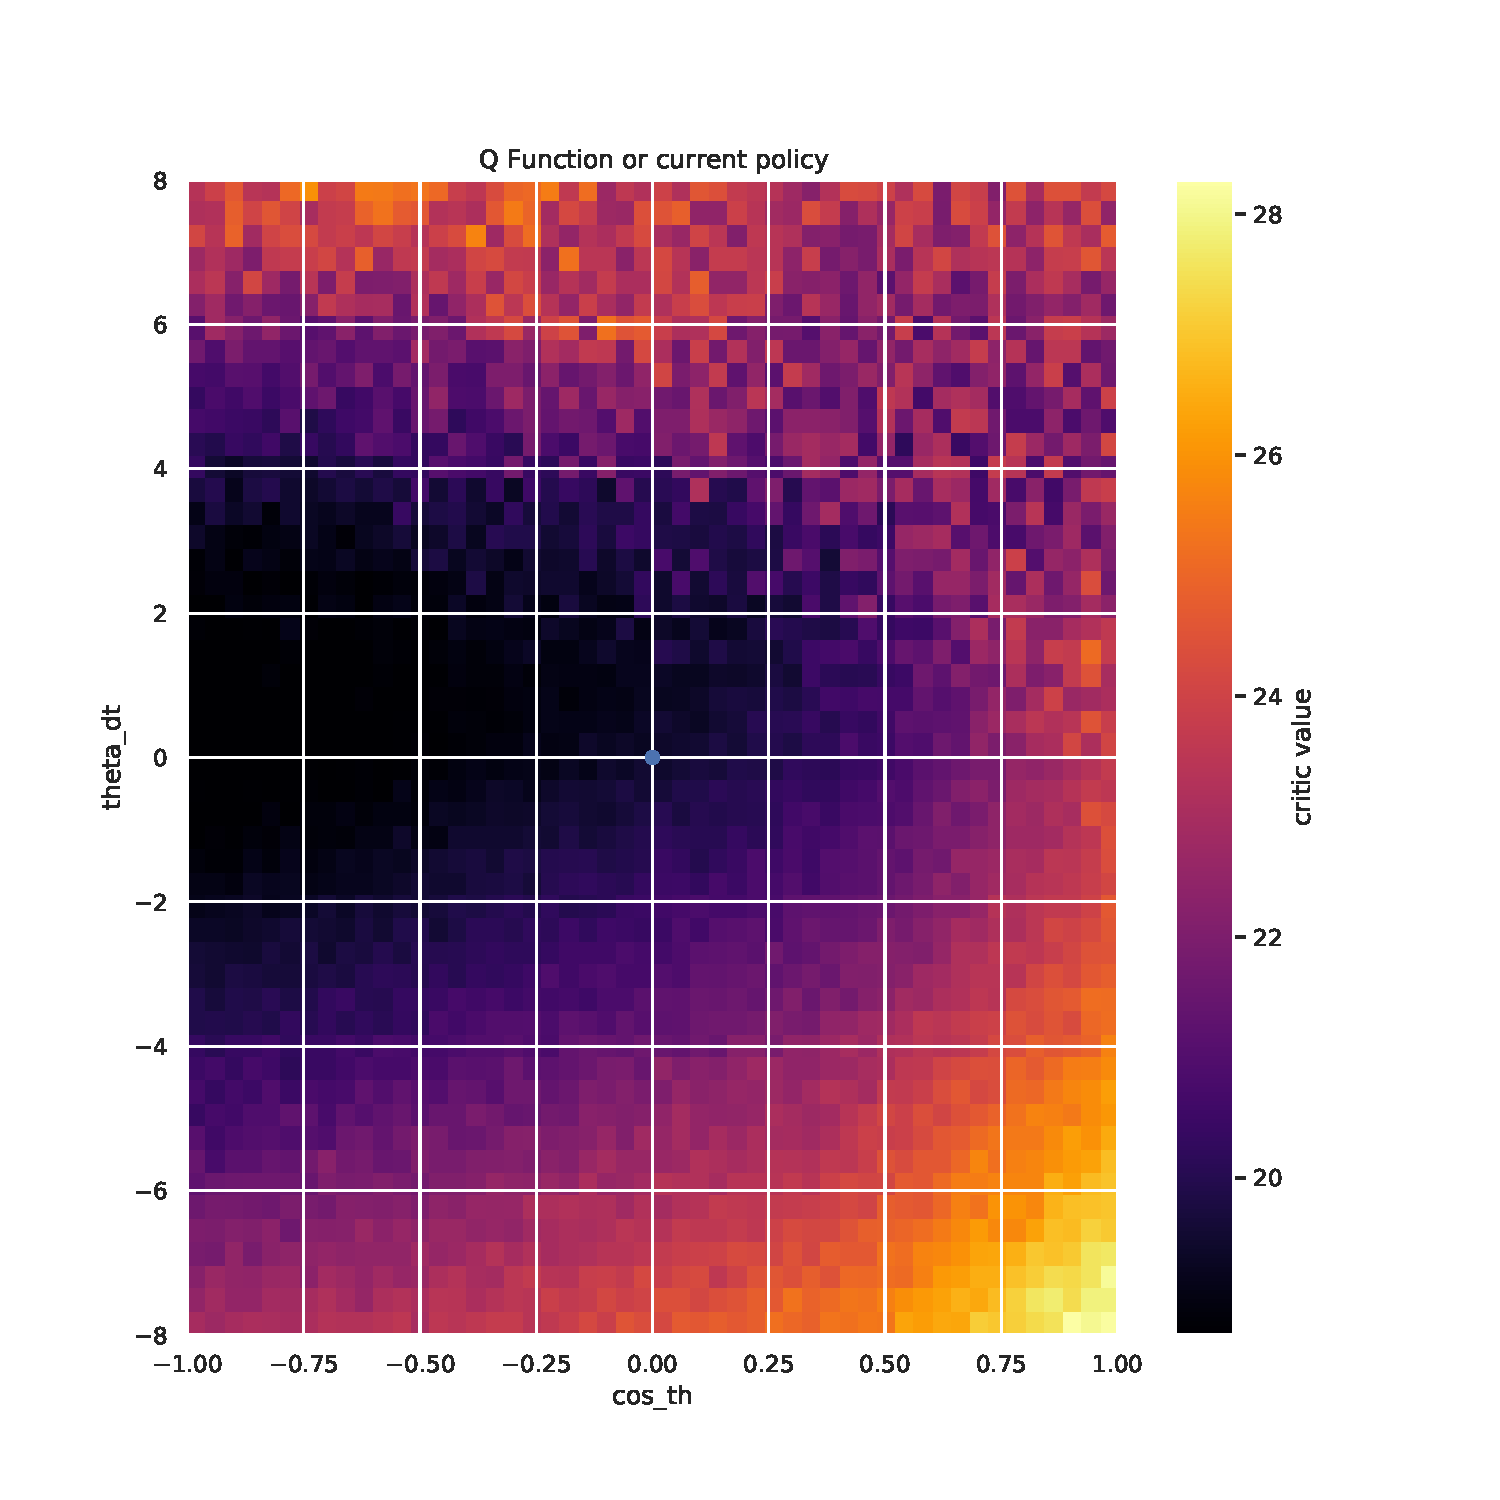
\includegraphics[width=\textwidth]{figures/iteration3/0_critic_normalize_post_Pendulum-v0.pdf}
        \caption{Critique entraînée}
    \end{subfigure}
    \caption{Valeurs de l'acteur et de la critique avec la méthode normalize pour le calcul de la récompense}
    \label{fig:itr3_normalize}
\end{figure}

La méthode \emph{normalize} ne présente toujours pas d'acteur entraîné correctement. Dans ce cas, la politique va faire tourner le pendule à la même vitesse et dans le même sens peu importe son état.

La critique, quant à elle, semble bien défavoriser le fait d'être en bas du pendule mais préfère être à grande vitesse une fois en haut. Cela n'est donc toujours pas ce que nous attendons.
\subsection{Itération n°4}

\subsubsection{Configuration, modifications et résultats attendus}

Nous avons une autre idée de la cause de ces résultats décevants. Il pourrait s'agir d'un manque d'exploration. Donc nous essayons d'utiliser un nombre bien plus grand d'épisodes. Nous prenons 800 cycles composés de 200 épisodes.

Nous espérons voir une décroissance de la perte de la critique et de la politique et une augmentation de la récompense. Si c'est le cas, alors le problème est effectivement un manque de données d'exploration. Si nous n'obtenons pas de résultats concluants nous nous pencherons sur une nouvelle implémentation d'algorithme par renforcement profond.

\subsubsection{Analyse}

\begin{figure}[H]
    \centering
    \begin{subfigure}{0.3\textwidth}
        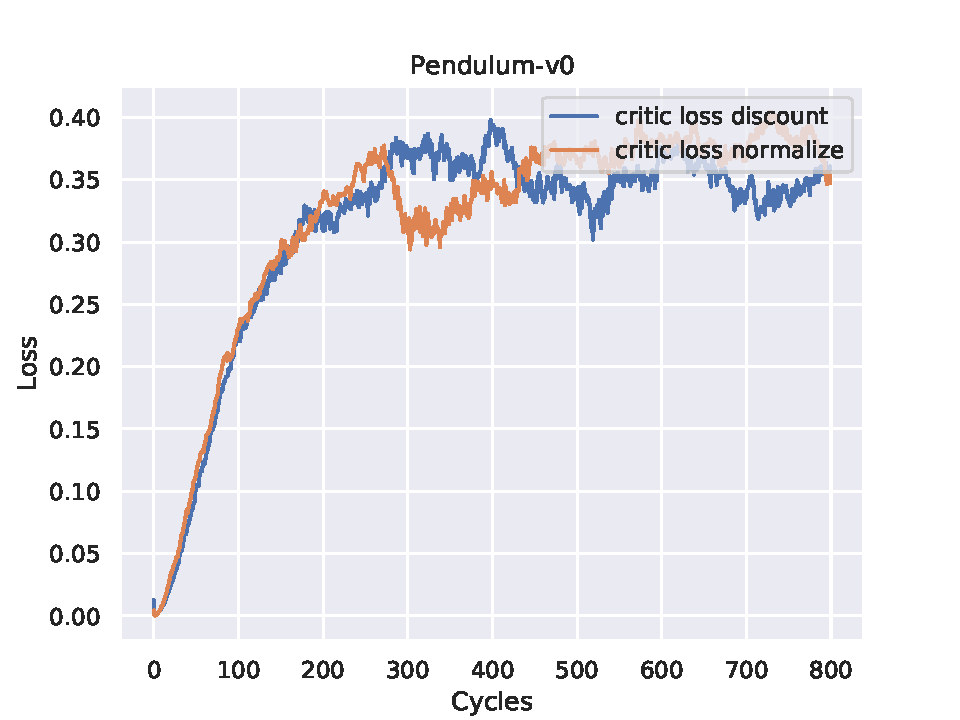
\includegraphics[width=\textwidth]{figures/iteration4/critic_loss_Pendulum-v0_pg_dataset_td_eval_True_cycles_800_trajs_200_batches_20_gamma_0.99_nstep_5_lr_act_0.01_lr_critic_0.01pg.pdf}
        \caption{Fonction de perte de la critique}
    \end{subfigure}
    \begin{subfigure}{0.3\textwidth}
        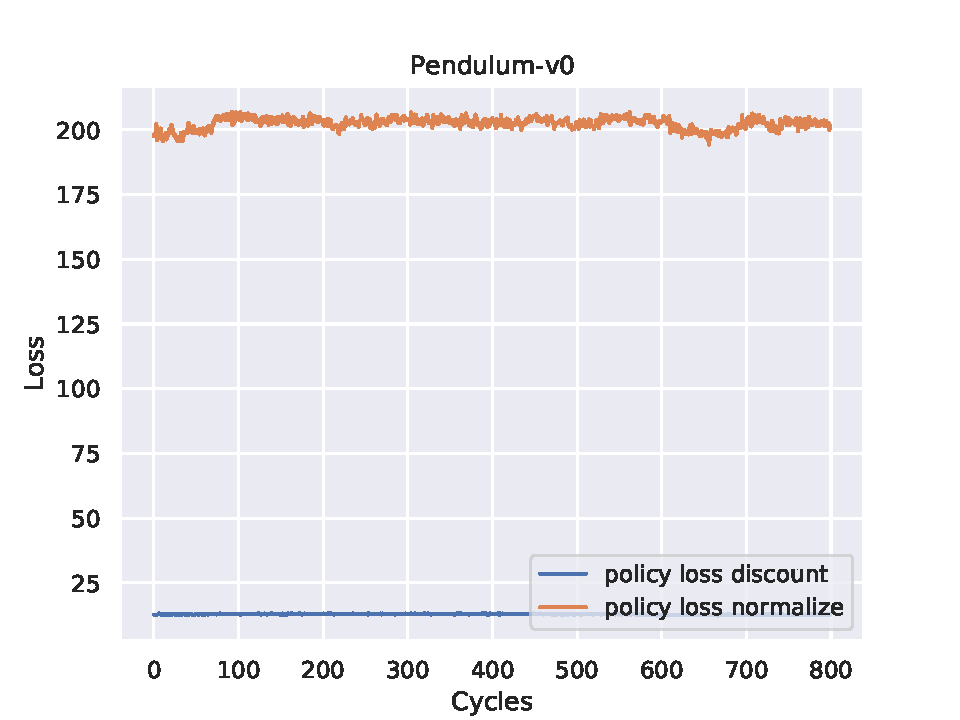
\includegraphics[width=\textwidth]{figures/iteration4/policy_loss_Pendulum-v0_pg_dataset_td_eval_True_cycles_800_trajs_200_batches_20_gamma_0.99_nstep_5_lr_act_0.01_lr_critic_0.01pg.pdf}
        \caption{Fonction de perte de la politique}
    \end{subfigure}
    \begin{subfigure}{0.3\textwidth}
        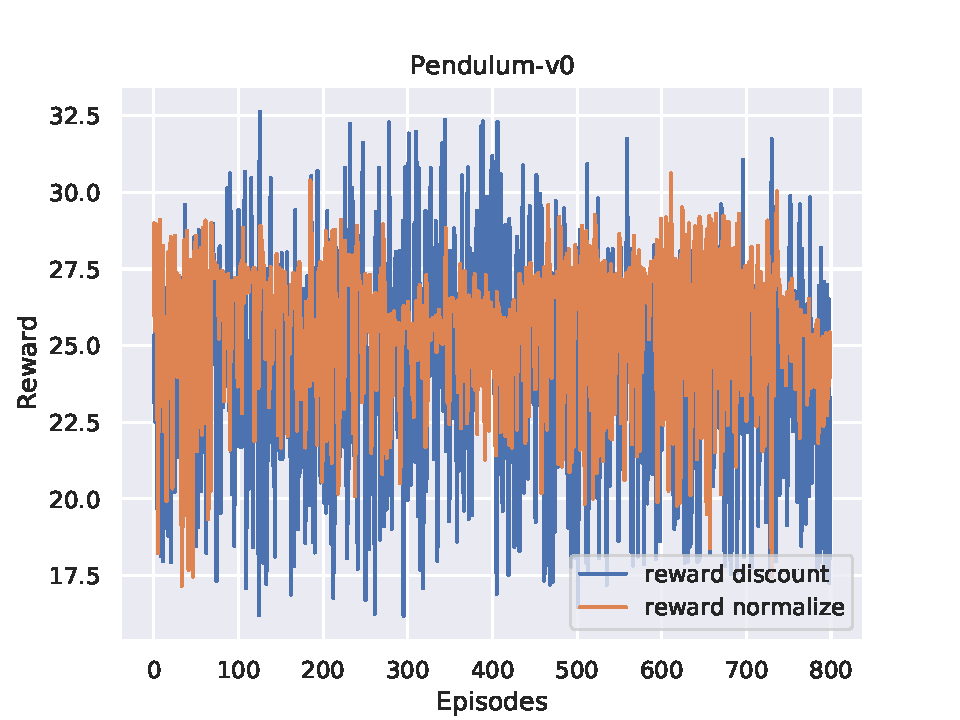
\includegraphics[width=\textwidth]{figures/iteration4/rewards_Pendulum-v0_pg_dataset_td_eval_True_cycles_800_trajs_200_batches_20_gamma_0.99_nstep_5_lr_act_0.01_lr_critic_0.01.pdf}
        \caption{Récompenses des épisodes}
    \end{subfigure}
    \caption{Résultats obtenus pour la critique, la politique et la récompense}
    \label{fig:itr4_results}
\end{figure}

Malgré l'augmentation de l'exploration et du nombre de trajectoire par \emph{batch}, les résultats obtenus sont très similaires et rien ne s'est amélioré. Nous attendons toujours que la fonction perte de la critique finisse par décroître. Le comportement singulier des pertes sur la politique nous interroge toujours autant. Enfin, la récompense n'a pas évoluer malgré le grand nombre d'itérations.

\begin{figure}[H]
    \centering
    \begin{subfigure}{0.3\textwidth}
        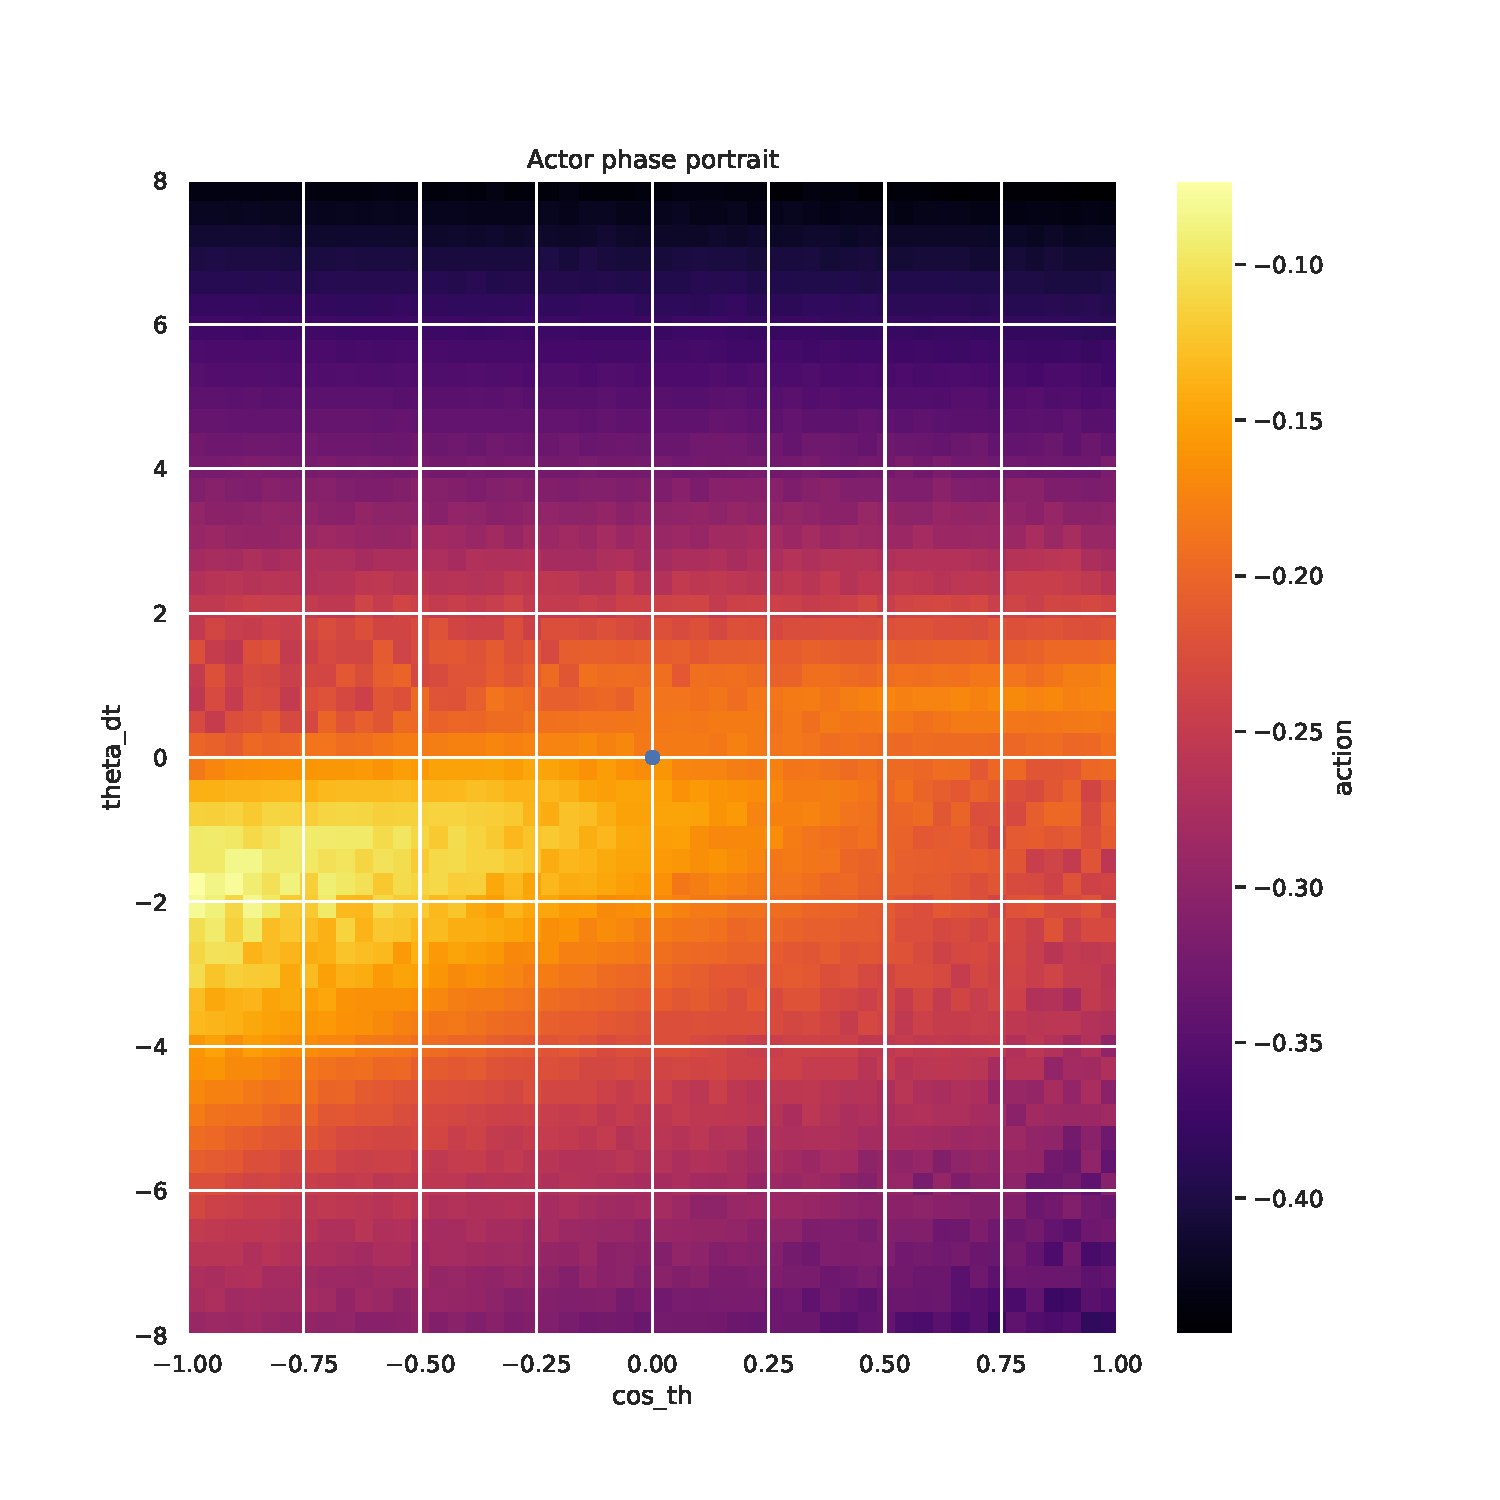
\includegraphics[width=\textwidth]{figures/iteration4/0_actor_discount__ante_Pendulum-v0.pdf}
        \caption{Acteur naïf}
    \end{subfigure}
    \begin{subfigure}{0.3\textwidth}
        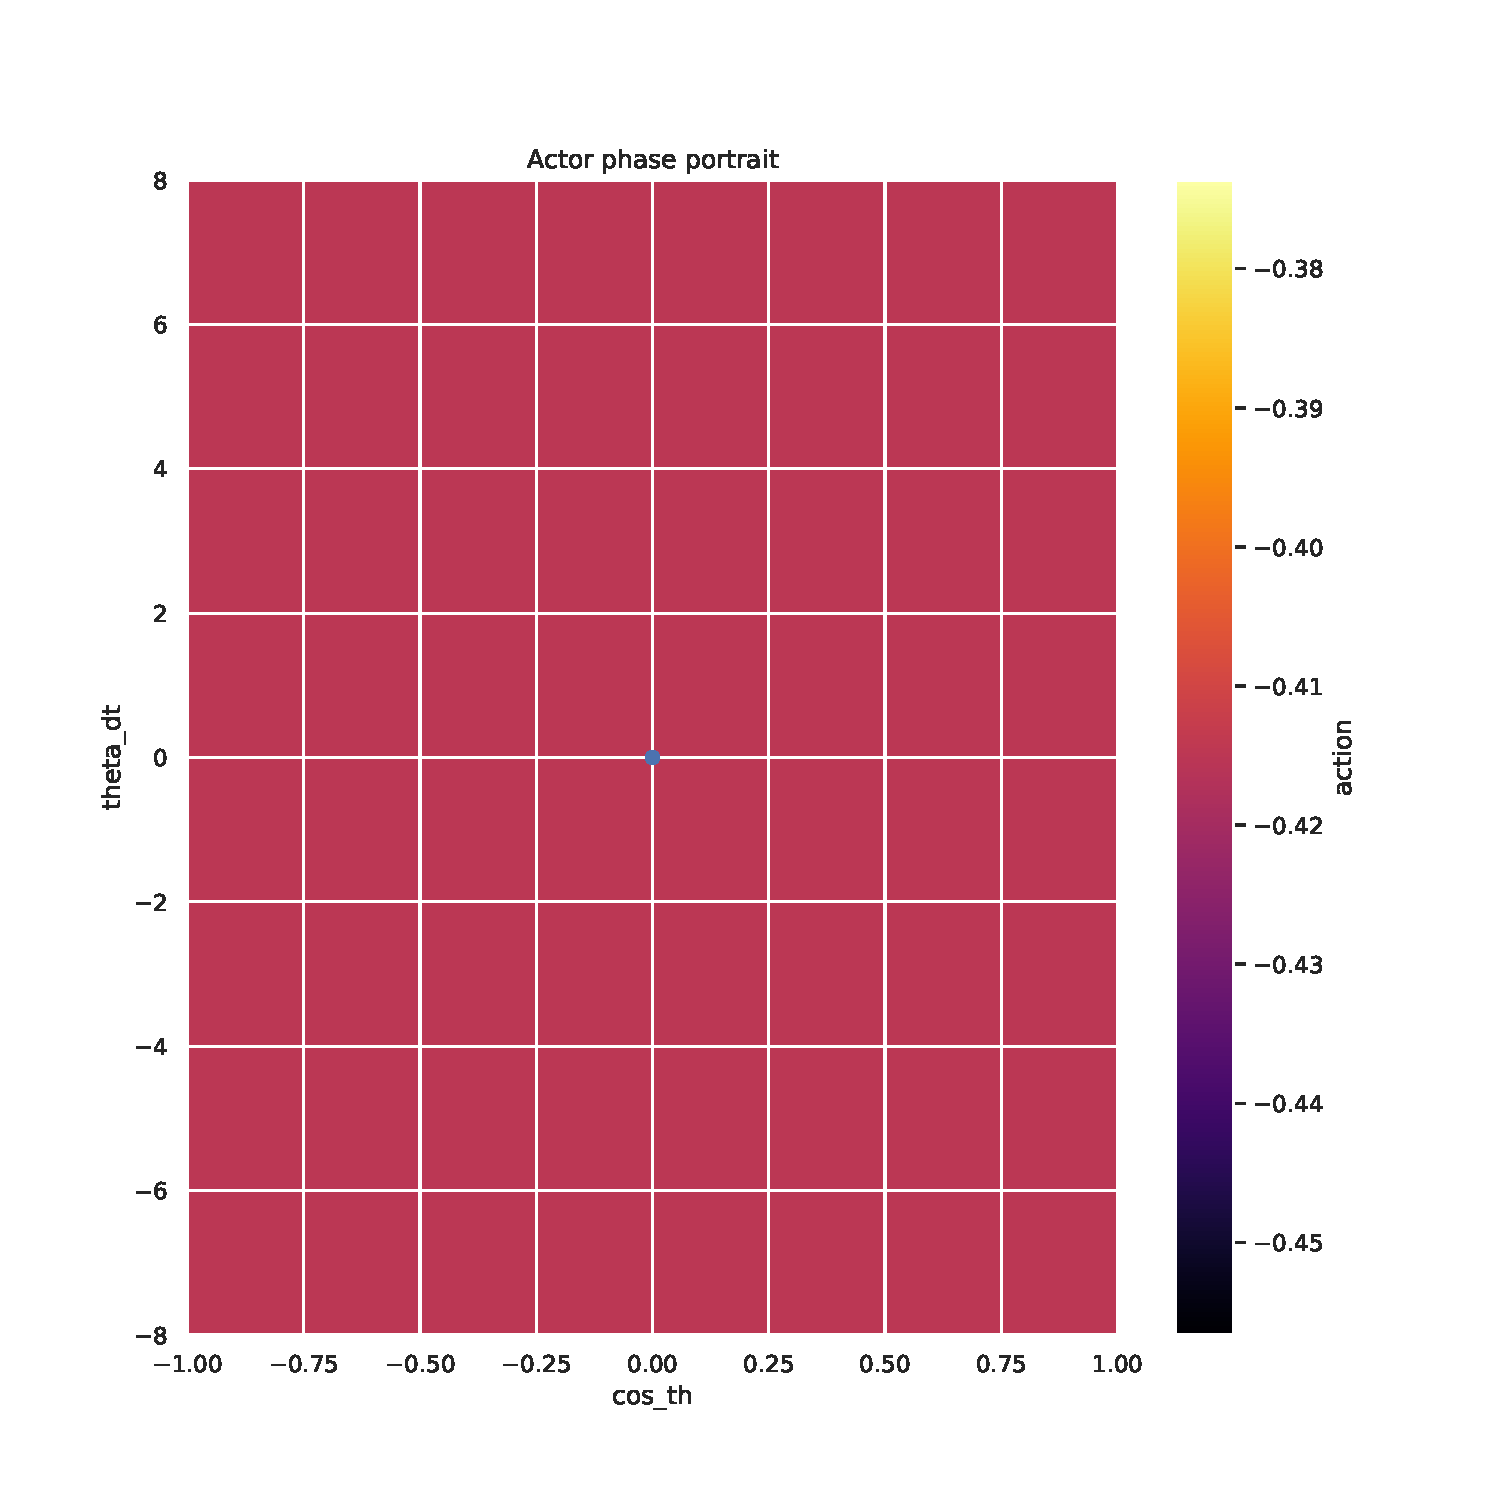
\includegraphics[width=\textwidth]{figures/iteration4/0_actor_discount__post_Pendulum-v0.pdf}
        \caption{Acteur entraîné}
    \end{subfigure}
    \begin{subfigure}{0.3\textwidth}
        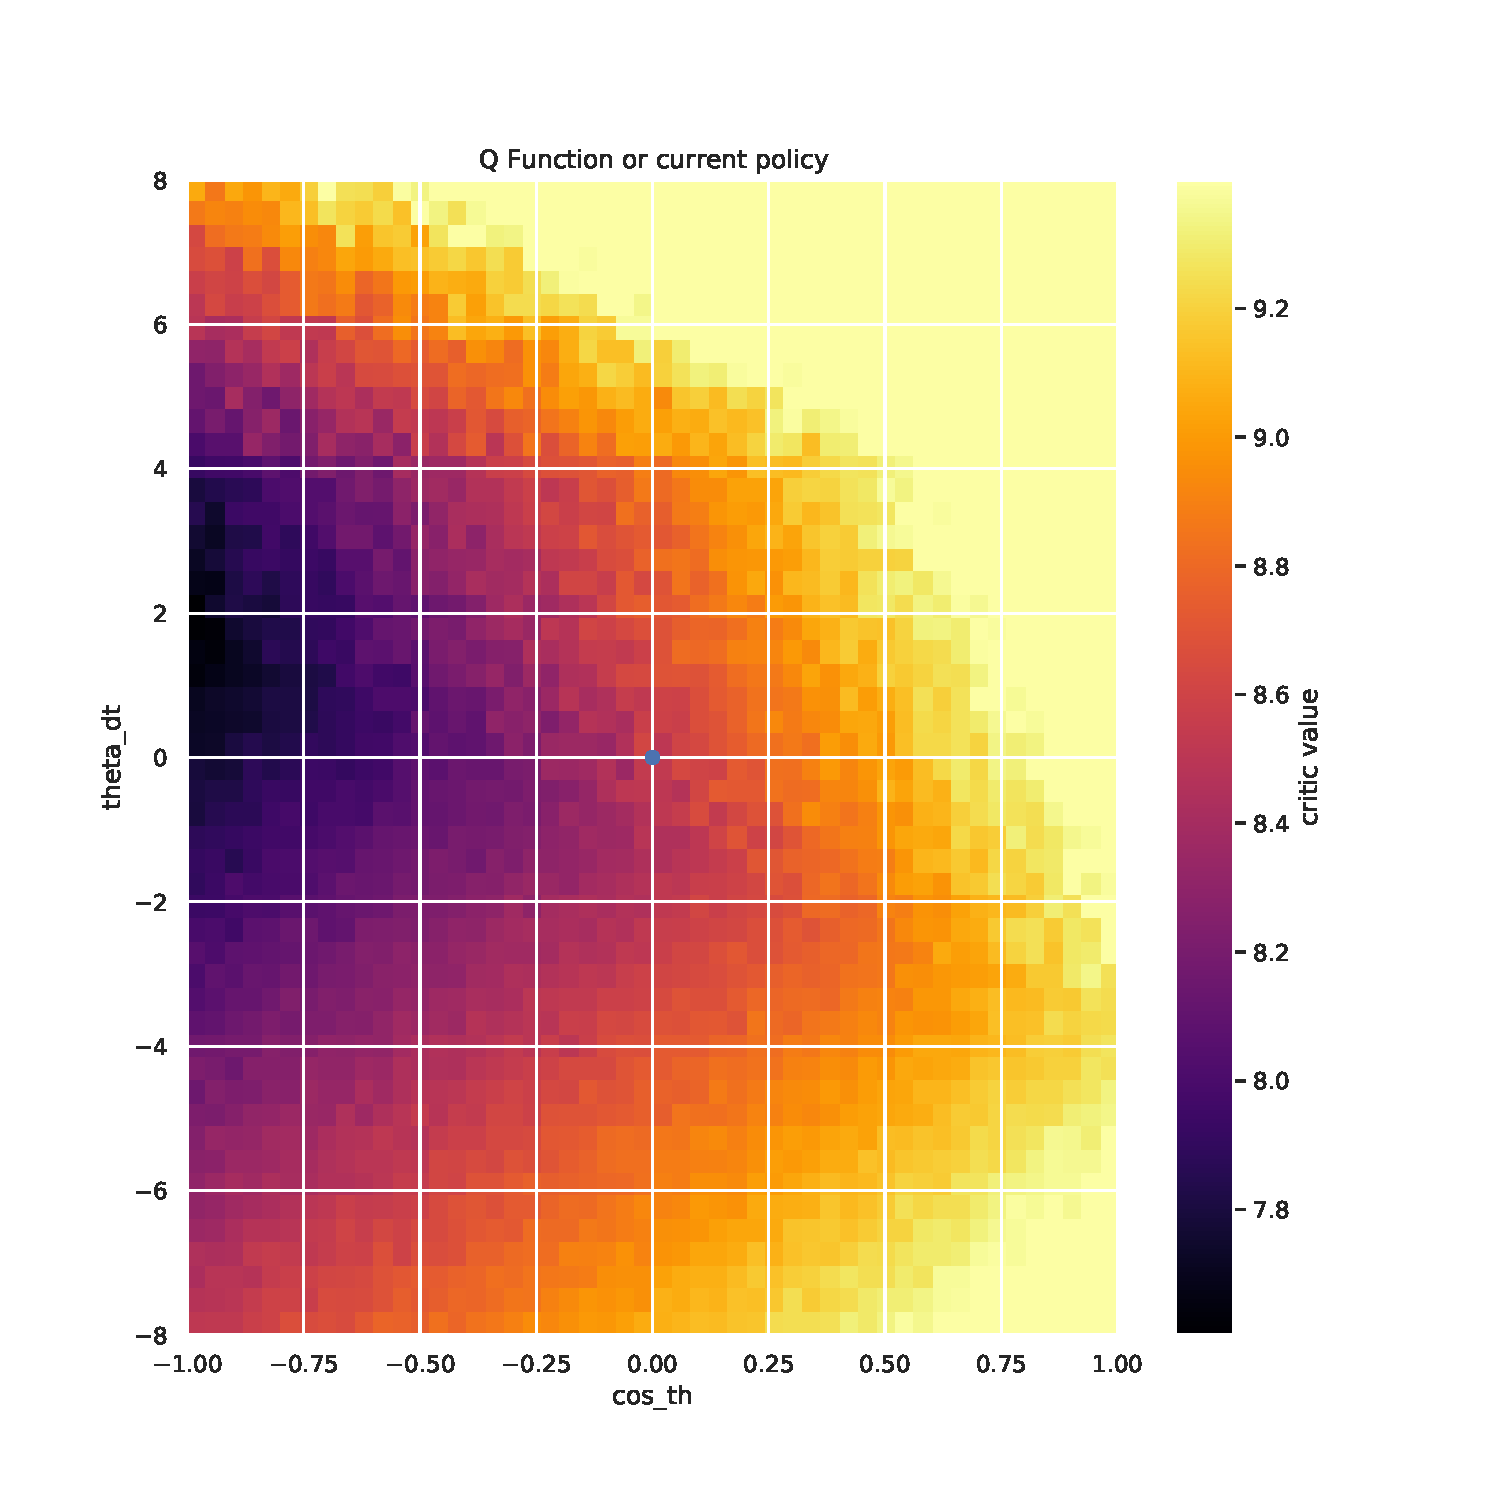
\includegraphics[width=\textwidth]{figures/iteration4/0_critic_discount_post_Pendulum-v0.pdf}
        \caption{Critique entraînée}
    \end{subfigure}
    \caption{Valeurs de l'acteur et de la critique avec la méthode discount pour le calcul de la récompense}
    \label{fig:itr4_discount}
\end{figure}

\begin{figure}[H]
    \centering
    \begin{subfigure}{0.3\textwidth}
        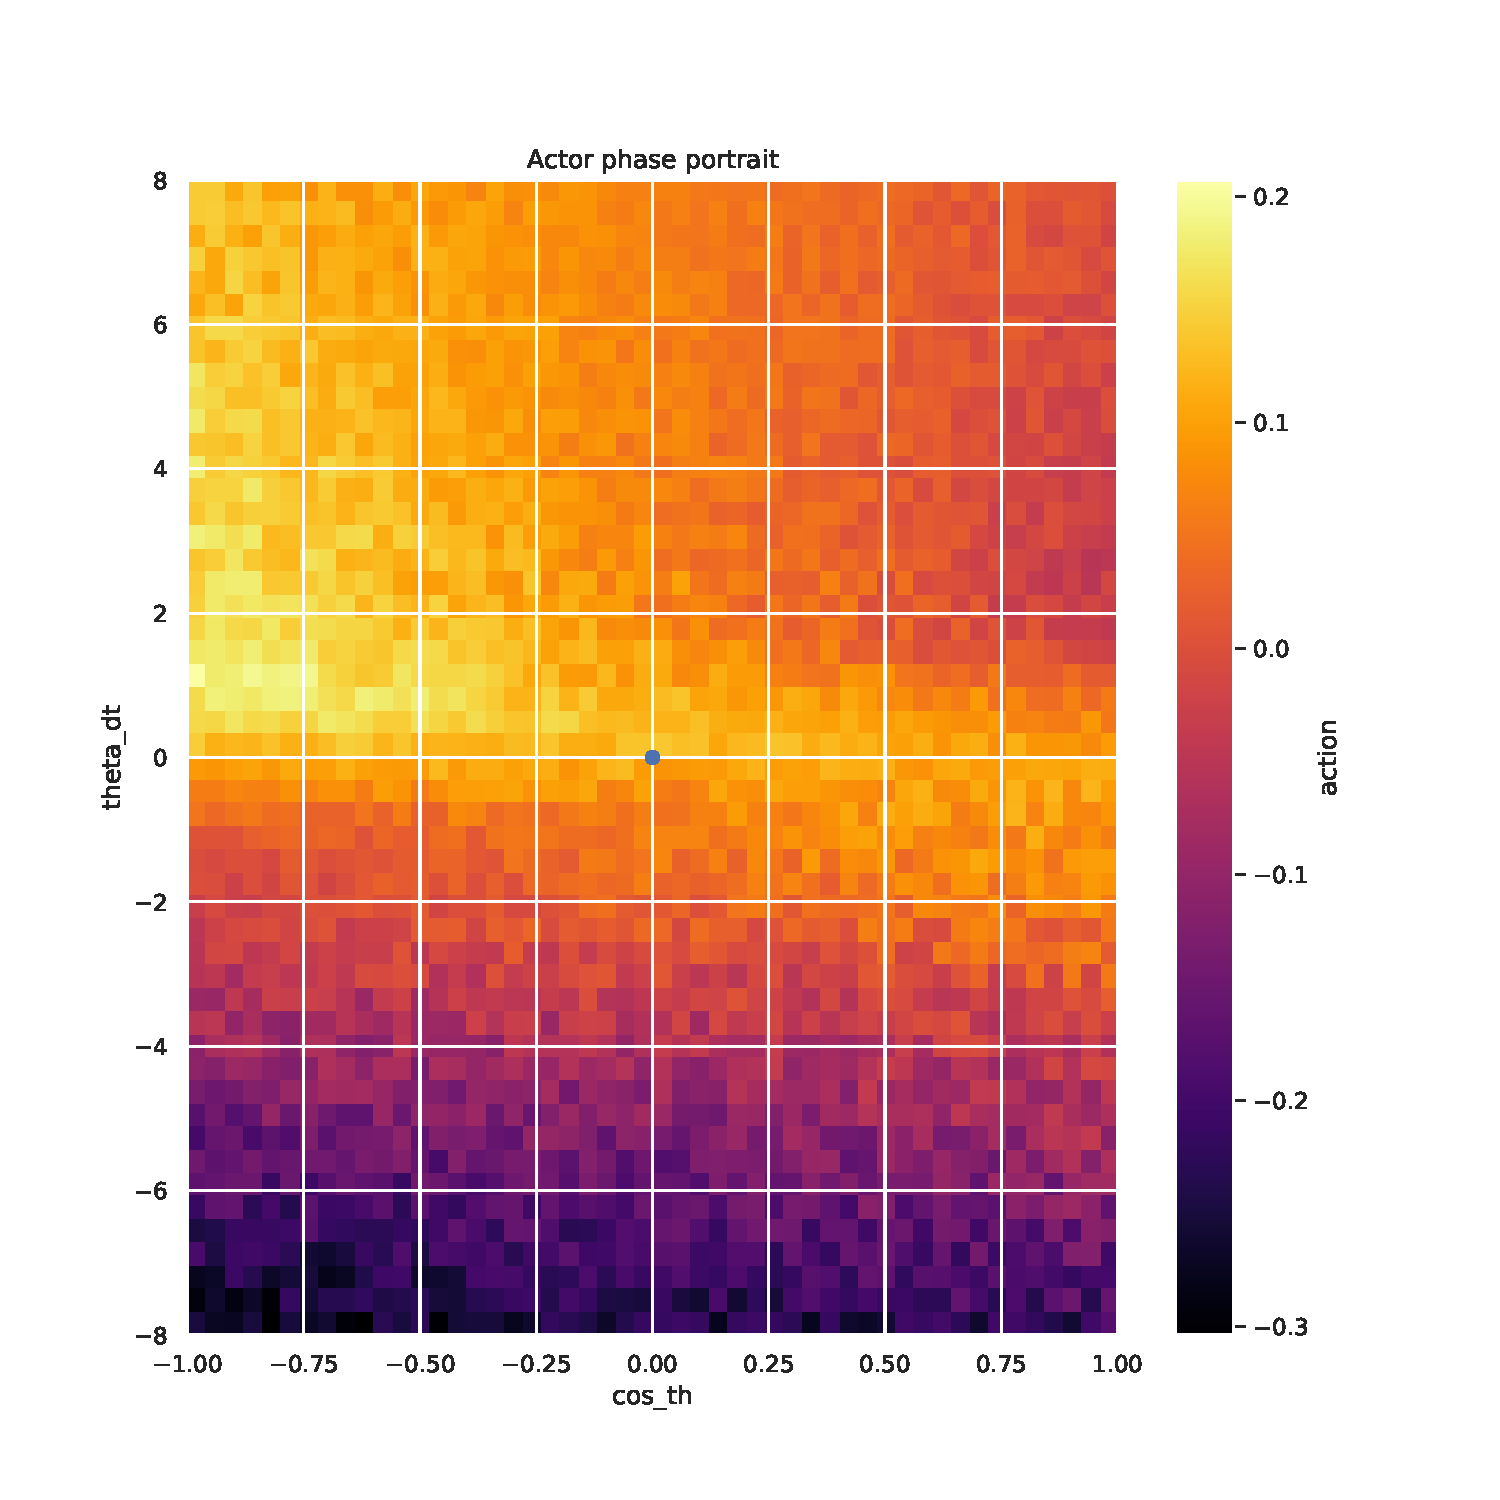
\includegraphics[width=\textwidth]{figures/iteration4/0_actor_normalize__ante_Pendulum-v0.pdf}
        \caption{Acteur naïf}
    \end{subfigure}
    \begin{subfigure}{0.3\textwidth}
        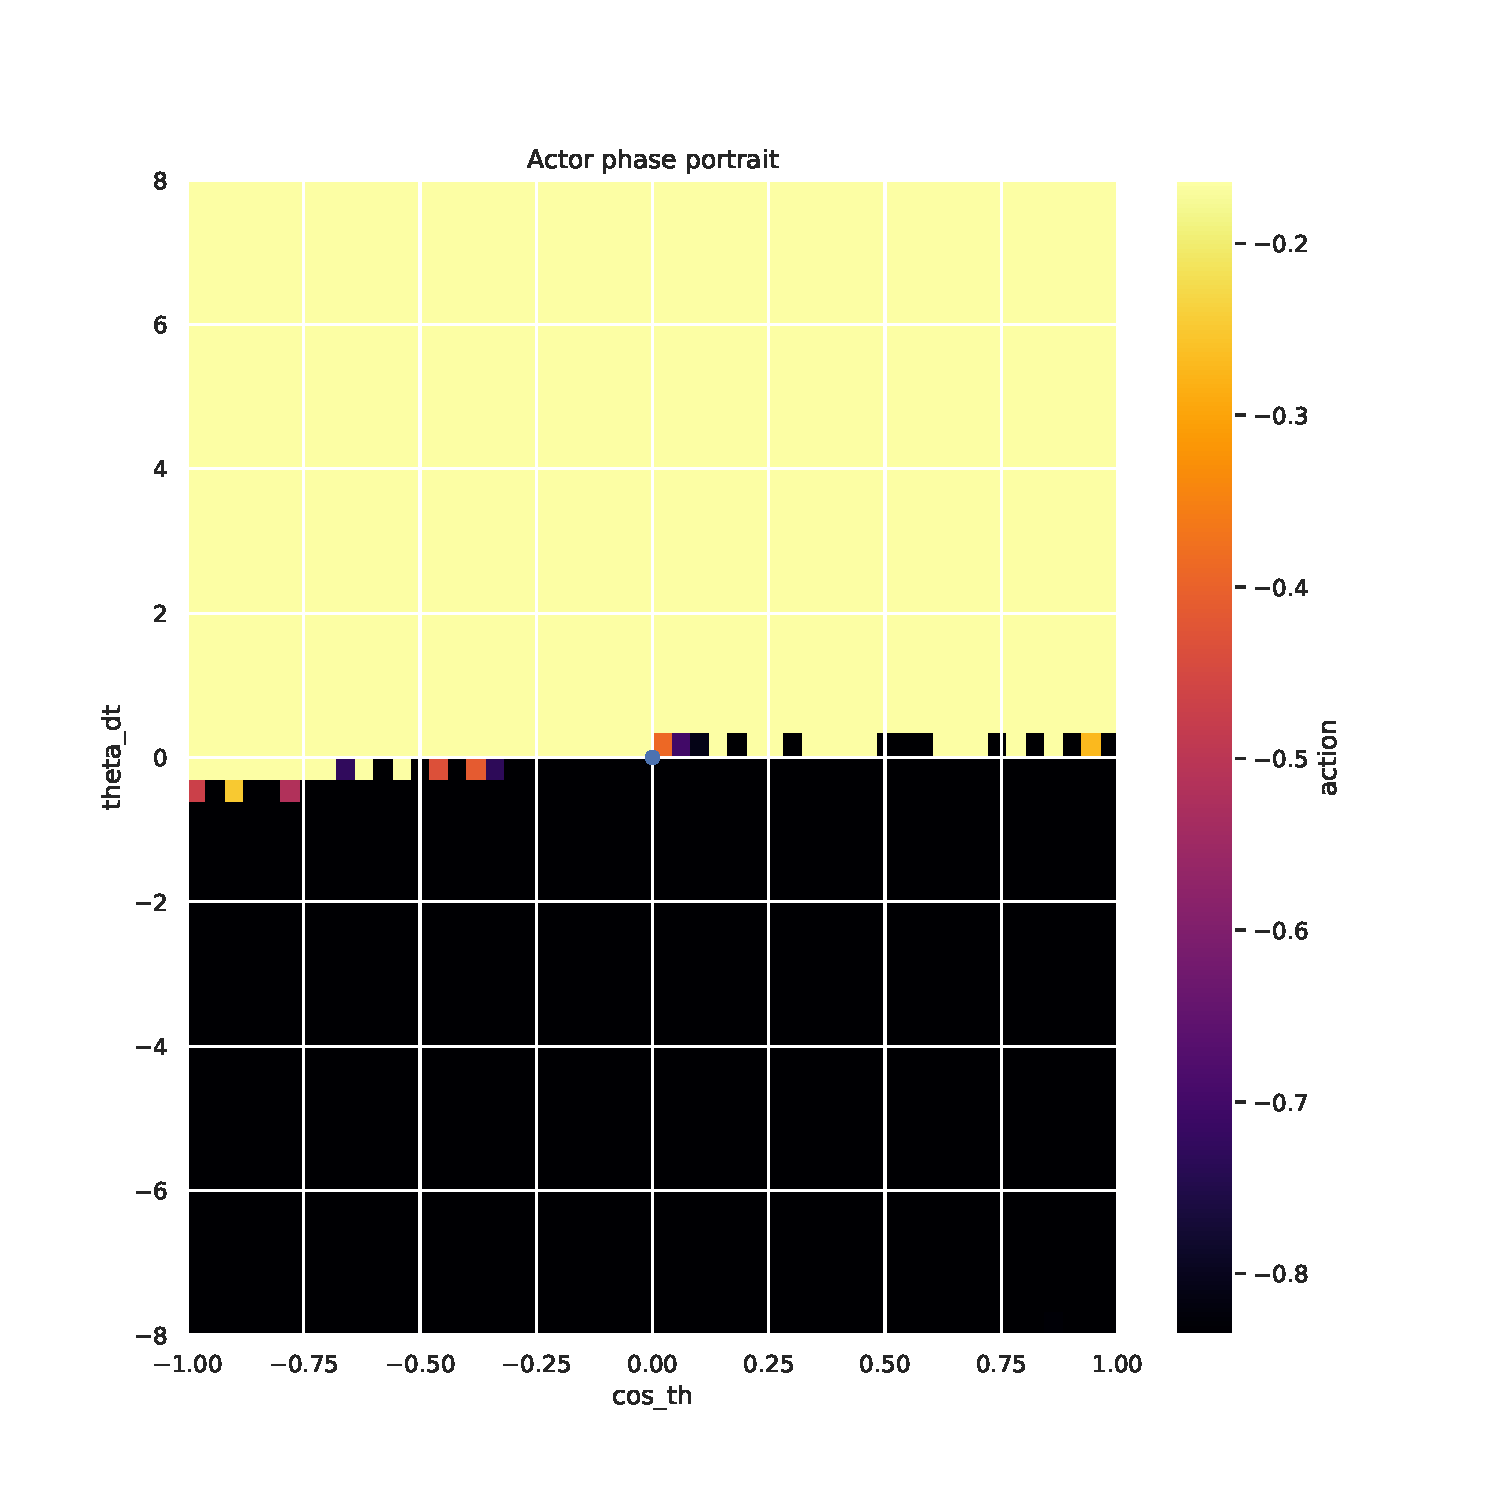
\includegraphics[width=\textwidth]{figures/iteration4/0_actor_normalize__post_Pendulum-v0.pdf}
        \caption{Acteur entraîné}
    \end{subfigure}
    \begin{subfigure}{0.3\textwidth}
        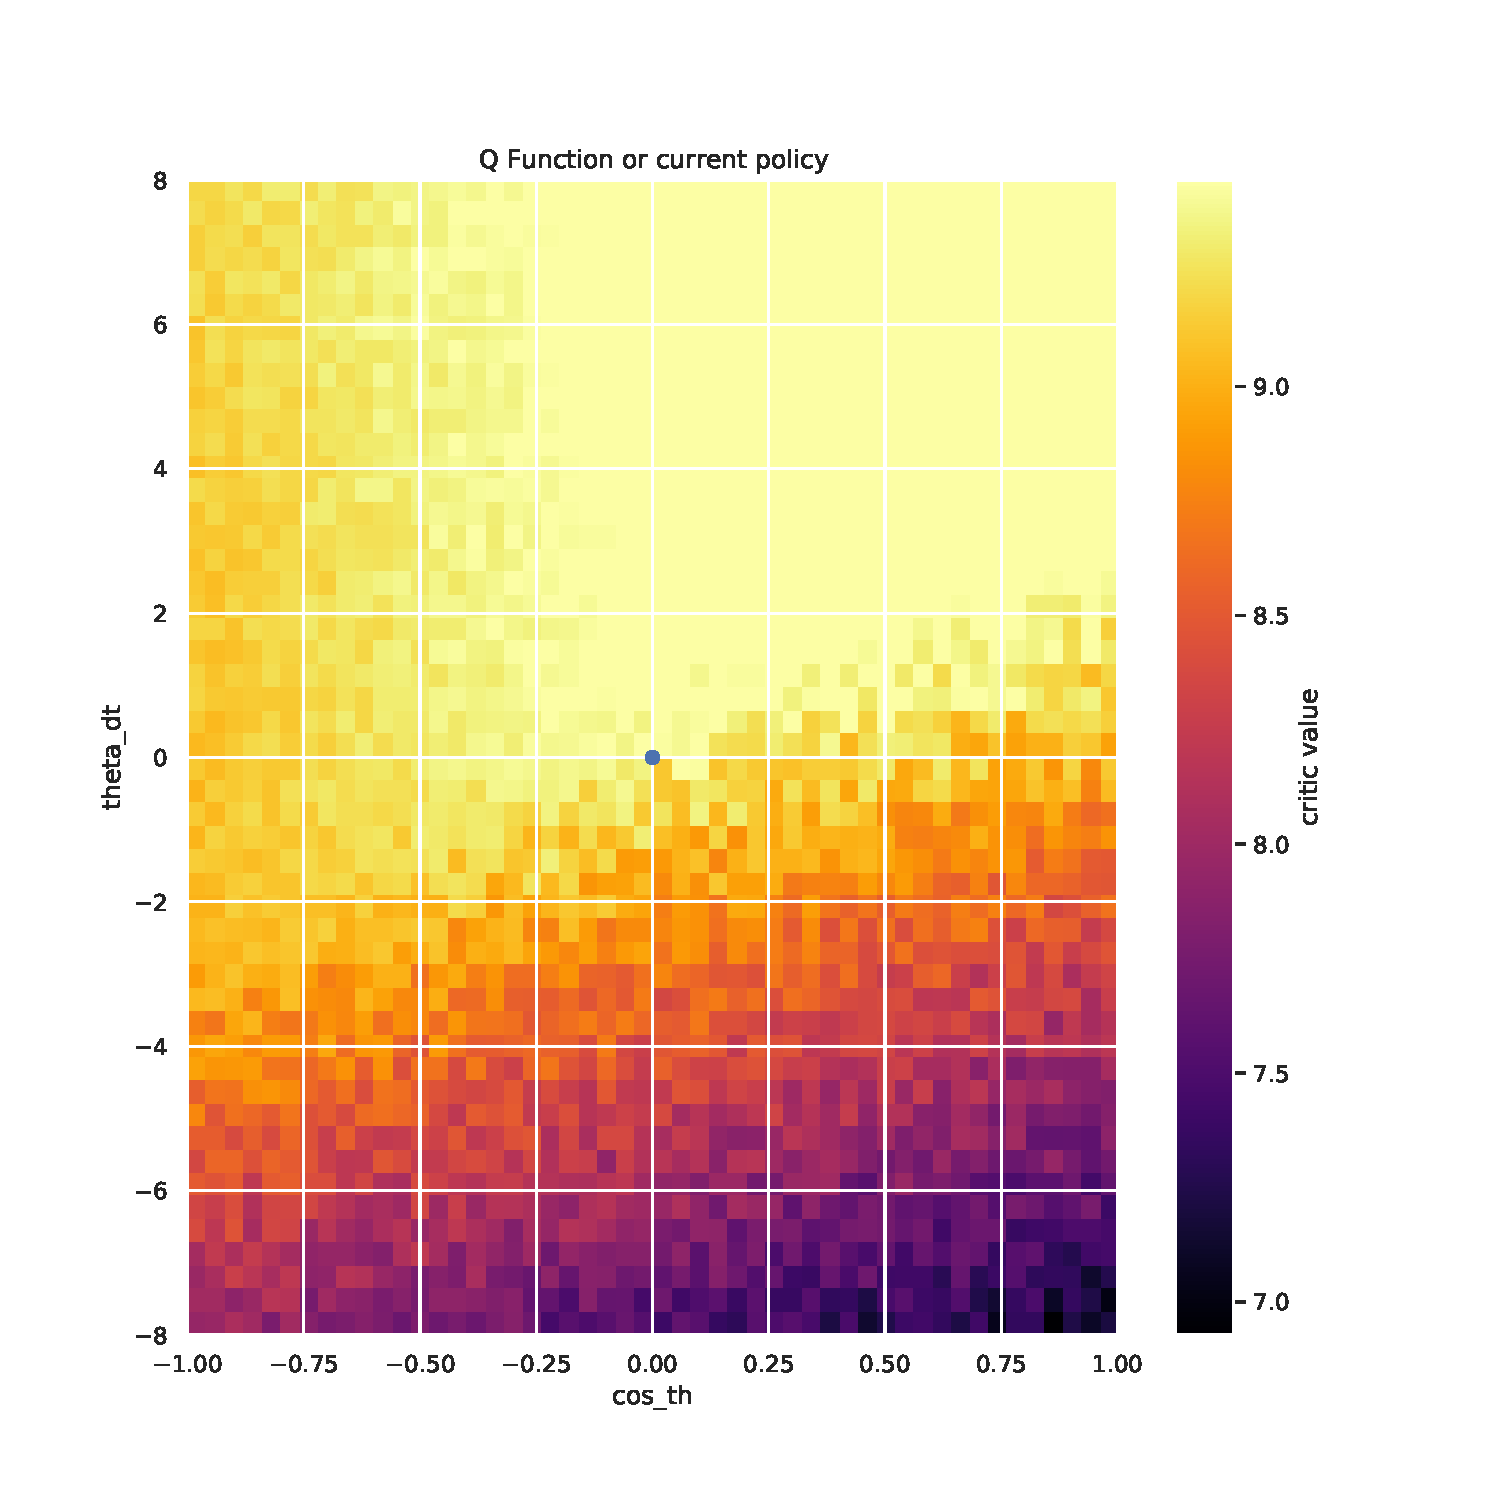
\includegraphics[width=\textwidth]{figures/iteration4/0_critic_normalize_post_Pendulum-v0.pdf}
        \caption{Critique entraînée}
    \end{subfigure}
    \caption{Valeurs de l'acteur et de la critique avec la méthode discount pour le calcul de la récompense}
    \label{fig:itr4_normalize}
\end{figure}

Ces graphes sur les figures~\ref{fig:itr4_discount} et \ref{fig:itr4_normalize} confirment que le problème ne vient pas de l'exploration mais plutôt de l'apprentissage en lui-même. Le problème est surement lié à l'implémentation. Puisque le projet contient un nombre conséquent de classes, nous n'approfondirons pas plus les recherches et nous implémentons un algorithme de \emph{policy grandient}.

\section{Algorithme \emph{Soft Actor Critic}}
Nous décidons d'implémenter un algorithme \emph{state of the art}. Nous avons donc le choix entre les algorithmes D4PG, TD3, TRPO et SAC. Nous choisissons l'algorithme \emph{Soft Actor Critic} parce qu'il présente un bon compromis entre TRPO qui est stable mais qui sous exploite ses échantillons, et TD3 qui est instable et exploite au mieux les échantillons. SAC réunit le meilleur des deux mondes en étant stable et en utilisant efficacement un \emph{replay buffer}. La gestion de l'entropie sur le domaine des actions permet de favoriser l'exploration et d'éviter une politique stochastique. L'utilisation de deux critiques le rend plus résistant à l'\emph{over-estimation bias}.

Nous avons trouvé un \href{https://github.com/seungeunrho/minimalRL/blob/master/sac.py}{dépôt sur Github} qui propose une implémentation relativement légère et simple à comprendre rédigée par \href{https://github.com/seungeunrho}{seungeunrho}. Celle-ci est proche de celle proposée par \href{https://spinningup.openai.com/en/latest/algorithms/sac.html}{Spinning Up}. Cependant, cette version de l'algorithme apprend aussi le paramètre $\alpha$.

Nous avons restructuré ce code et y avons incorporé la visualisation du dépôt donné pour ce TME. Nous nous sommes assuré que la politique générée puisse être utilisée dans \emph{evaluator.py}. Enfin, nous avons changé les arguments du programme pour qu'ils correspondent aux hyper-paramètres.
\subsection{Résultats obtenus avec les paramètres initiaux}

\begin{table}[H]
        \centering
        \begin{tabular}{@{}l l l@{}}
            \toprule
            \textbf{Simulation} & Nombre d'épisodes & 400 \\
            & Seuil de mise à jour & 1000 \\
            & Nombre de mise à jour & 20 \\
            & Taille du \emph{mini batch} & 32 \\
            & Nombre de pas par épisode & 200 \\ \midrule
            \textbf{Politique} & Fréquence d'apprentissage & 0,0005\\
            & $\alpha_{0}$ & 0,01\\
            & Fréquence d'apprentissage de $\alpha$ & 0,0001\\
            & Entropie ciblée pour $\alpha$ & -1\\ \midrule
            \textbf{Critique} & Fréquence d'apprentissage & 0,001\\
            & \emph{Discount factor} $\gamma$ & 0,98\\
            & $\tau$ & 0,01\\
            \bottomrule
        \end{tabular}
    \caption{Tableaux de la configuration initiale du \emph{Soft Actor Critic}}\label{tab:sac:initial_settings}
\end{table}
\end{document}
